% Options for packages loaded elsewhere
\PassOptionsToPackage{unicode}{hyperref}
\PassOptionsToPackage{hyphens}{url}
%
\documentclass[
]{article}
\usepackage{amsmath,amssymb}
\usepackage{iftex}
\ifPDFTeX
  \usepackage[T1]{fontenc}
  \usepackage[utf8]{inputenc}
  \usepackage{textcomp} % provide euro and other symbols
\else % if luatex or xetex
  \usepackage{unicode-math} % this also loads fontspec
  \defaultfontfeatures{Scale=MatchLowercase}
  \defaultfontfeatures[\rmfamily]{Ligatures=TeX,Scale=1}
\fi
\usepackage{lmodern}
\ifPDFTeX\else
  % xetex/luatex font selection
\fi
% Use upquote if available, for straight quotes in verbatim environments
\IfFileExists{upquote.sty}{\usepackage{upquote}}{}
\IfFileExists{microtype.sty}{% use microtype if available
  \usepackage[]{microtype}
  \UseMicrotypeSet[protrusion]{basicmath} % disable protrusion for tt fonts
}{}
\makeatletter
\@ifundefined{KOMAClassName}{% if non-KOMA class
  \IfFileExists{parskip.sty}{%
    \usepackage{parskip}
  }{% else
    \setlength{\parindent}{0pt}
    \setlength{\parskip}{6pt plus 2pt minus 1pt}}
}{% if KOMA class
  \KOMAoptions{parskip=half}}
\makeatother
\usepackage{xcolor}
\usepackage{longtable,booktabs,array}
\usepackage{calc} % for calculating minipage widths
% Correct order of tables after \paragraph or \subparagraph
\usepackage{etoolbox}
\makeatletter
\patchcmd\longtable{\par}{\if@noskipsec\mbox{}\fi\par}{}{}
\makeatother
% Allow footnotes in longtable head/foot
\IfFileExists{footnotehyper.sty}{\usepackage{footnotehyper}}{\usepackage{footnote}}
\makesavenoteenv{longtable}
\usepackage{graphicx}
\makeatletter
\def\maxwidth{\ifdim\Gin@nat@width>\linewidth\linewidth\else\Gin@nat@width\fi}
\def\maxheight{\ifdim\Gin@nat@height>\textheight\textheight\else\Gin@nat@height\fi}
\makeatother
% Scale images if necessary, so that they will not overflow the page
% margins by default, and it is still possible to overwrite the defaults
% using explicit options in \includegraphics[width, height, ...]{}
\setkeys{Gin}{width=\maxwidth,height=\maxheight,keepaspectratio}
% Set default figure placement to htbp
\makeatletter
\def\fps@figure{htbp}
\makeatother
\setlength{\emergencystretch}{3em} % prevent overfull lines
\providecommand{\tightlist}{%
  \setlength{\itemsep}{0pt}\setlength{\parskip}{0pt}}
\setcounter{secnumdepth}{-\maxdimen} % remove section numbering
\ifLuaTeX
\usepackage[bidi=basic]{babel}
\else
\usepackage[bidi=default]{babel}
\fi
\babelprovide[main,import]{french}
% get rid of language-specific shorthands (see #6817):
\let\LanguageShortHands\languageshorthands
\def\languageshorthands#1{}
\makeatletter
\@ifpackageloaded{subfig}{}{\usepackage{subfig}}
\@ifpackageloaded{caption}{}{\usepackage{caption}}
\captionsetup[subfloat]{margin=0.5em}
\AtBeginDocument{%
\renewcommand*\figurename{Figure}
\renewcommand*\tablename{Table}
}
\AtBeginDocument{%
\renewcommand*\listfigurename{List of Figures}
\renewcommand*\listtablename{List of Tables}
}
\newcounter{pandoccrossref@subfigures@footnote@counter}
\newenvironment{pandoccrossrefsubfigures}{%
\setcounter{pandoccrossref@subfigures@footnote@counter}{0}
\begin{figure}\centering%
\gdef\global@pandoccrossref@subfigures@footnotes{}%
\DeclareRobustCommand{\footnote}[1]{\footnotemark%
\stepcounter{pandoccrossref@subfigures@footnote@counter}%
\ifx\global@pandoccrossref@subfigures@footnotes\empty%
\gdef\global@pandoccrossref@subfigures@footnotes{{##1}}%
\else%
\g@addto@macro\global@pandoccrossref@subfigures@footnotes{, {##1}}%
\fi}}%
{\end{figure}%
\addtocounter{footnote}{-\value{pandoccrossref@subfigures@footnote@counter}}
\@for\f:=\global@pandoccrossref@subfigures@footnotes\do{\stepcounter{footnote}\footnotetext{\f}}%
\gdef\global@pandoccrossref@subfigures@footnotes{}}
\@ifpackageloaded{float}{}{\usepackage{float}}
\floatstyle{ruled}
\@ifundefined{c@chapter}{\newfloat{codelisting}{h}{lop}}{\newfloat{codelisting}{h}{lop}[chapter]}
\floatname{codelisting}{Listing}
\newcommand*\listoflistings{\listof{codelisting}{List of Listings}}
\makeatother
\ifLuaTeX
  \usepackage{selnolig}  % disable illegal ligatures
\fi
\usepackage{bookmark}
\IfFileExists{xurl.sty}{\usepackage{xurl}}{} % add URL line breaks if available
\urlstyle{same}
\hypersetup{
  pdftitle={Pig Boy 1986-2358 : quand l'écriture du numérique infléchit les voix du théâtre et de la radio},
  pdfauthor={Siham Maidon},
  pdflang={fr},
  hidelinks,
  pdfcreator={LaTeX via pandoc}}

\title{Pig Boy 1986-2358 : quand l'écriture du numérique infléchit les voix du théâtre et de la radio}
\author{Siham Maidon}
\date{09/09/2024}

\begin{document}
\maketitle

\subsection{Remerciements}\label{remerciements}

J'aimerais adresser tous mes remerciements à celles et ceux qui ont rendu la rédaction de ce mémoire possible, et qui en ont fait un chemin joyeux malgré les embûches. Un très grand merci...

À mes directeurices de mémoire, pour votre patience et vos conseils. Marion, pour vos cours qui font dérouler le fil de la pensée comme une pelote, ludiques. David, pour tes cours drôles, où tout est prétexte à création, expérimentations sonores.

À Anaïs, sans qui rien n'aurait été possible, pour tes encouragements infinis, ton expérience de la recherche forcée, de l'École, et pour ta très précieuse relecture, pleine d'une rigueur affectueuse. Pour tes plats et tes lettres aussi, ta présence réconfortante lors de l'écriture.

À William, pour tes conseils précieux, tes références inopinées et la pente politique émancipatrice sur laquelle tu me fais glisser sans violence. Parce que tu me tiens quand plus rien ne me tient, toujours.

À ma mère et à Nicolas, qui m'avez nourrie et logée pendant les dernières semaines de rédaction, palliant la dépendance infantile dans laquelle ce mémoire m'a ramenée. À toutes les villes, les lieux qui m'avez accueillie pendant ce travail.

À Lolita, pour ton compagnonnage qui chante et qui danse, qui guérit tous les maux et rit tous les mots. Pour ton ultime relecture, et d'être venue me sauver à la toute fin.

À tous·tes les auteurices, metteureuses en scène, les comédien·nes et les ingénieur·es du son qui avez accepté de me donner accès à vos œuvres pour constituer mon corpus et de répondre à mes questions. Qui m'avez laissée entrer dans votre univers. À Gwendoline Soublin, Christophe Hocké, Mathieu Touren, Philippe Mangenot, Noëlle Miral, Hélène Cerles, Romain Maurel, Lucie Monziès.

À l'équipe qui m'a joyeusement accueillie dans son projet, Clara, Alisma, Aurore, Maud, Théotime, Léo. Vous donnez sens à ma recherche et me permettez de l'aborder par la création, comme j'essaie toujours de le faire.

À Émi Lavigne-Matsuoka, tu me parles sans parler et tu m'a permis de détacher la voix de son phénomène sonore et de plonger dans ta langue pleine de corps toute cette année, et pour la vie.

À la bibliothèque universitaire de Paris 8, qui a tous les livres, tous les articles, toutes les thèses, et qui est encore là quand chacun·e part en vacances. Merci mille fois aux bibliothécaires et à leur travail minutieux.

À la revue Marges et à Jérôme Glicenstein, qui avez accepté ma proposition de communication et m'avez fait écrire un article avant ce mémoire, merci de m'avoir mise à l'ouvrage. À la licence Arts de Brest, qui se bat joyeusement pour un autre enseignement de l'art.

Aux équipes du théâtre Nicole Loraux, qui me faites rester, qui donnez sens à ma recherche, qui faites de moi la créatrice sonore que je suis aujourd'hui. Merci à Éric, mais aussi à Loman, Ève, Nicolas, Elsa, à tous·tes qui me faites confiance.

À Sylvain, qui m'aide à chaque fois à mettre en forme mes rendus dans des délais inacceptables.

\subsection{Préambule}\label{pruxe9ambule}

Lorsque j'ai terminé d'écouter la version radiophonique de \emph{Pig Boy 1986-2358} pour la première fois, je me suis dit que c'était l'objet le plus étrange et précieux qu'il m'avait été donné d'écouter ces dernières années en radio, de façon presque caricaturale le plus «~radiophonique~» aussi, et je remercie aujourd'hui Christophe Hocké et toute son équipe de l'avoir réalisé. Puis je me suis arrêtée sur cette phrase du générique~: «~une fiction sonore de Gwendoline Soublin~». Gwendoline Soublin, qui écrit des pièces de théâtre.

Lorsque j'ai terminé de lire le texte des éditions 34, j'étais tout aussi enthousiaste. Tout est écrit. Les choix, les commentaires, les jingles, les silences, tout. Ce qui m'avait semblé si spécifique au médium radiophonique de prime abord, et que j'avais donc considéré comme les interprétations du réalisateur, est scrupuleusement indiqué, avec le ressort ingénieux d'une mise en page proche des \emph{Calligrammes}. La partie 2, et je reprends ici les mots de Christophe Hocké, ressemble à une immense régie. Soit, alors la création radiophonique n'adapte pas tant le texte original, mais dans ce cas c'est parce qu'il constitue en lui-même une excellente partition radiophonique. Et pourtant, la pièce a été mise en scène. De nombreuses fois déjà, pour une pièce si jeune. Je n'y crois pas, et je veux voir. Sceptique, je m'engouffre dans les appels, les captations, des péripéties jusqu'à Saint-Hilaire-la-Croix pour aller assister à la dernière représentation du collectif Le Bruit des Cloches, avec toujours cette idée qu'aucune mise en scène ne pourrait faire face à la densité de la création sonore.

Et puis au fil de mes discussions avec tout le monde et chacun·e, je découvre la mise en scène du collectif Détour 21, qui s'écrit encore. Elle découle d'un projet de sortie d'école à l'ENSAD de Montpellier, où Clara Ménard avait proposé de monter la première partie pour son DET de mise en scène en 2022. La deuxième partie a aussi déjà été jouée deux fois au moment où j'en entends parler, et la troisième partie est en travail. Je rencontre Clara, qui m'accueille chaleureusement dans son projet, et ses fragments d'idées sonores résonnent instantanément avec ma pratique musicale, électronique, grésillante, à la recherche des bugs et de l'\emph{analog horror}. Je rejoins donc le bateau des résidences de sa petite équipe montpelliéraine. Nous cherchons encore à l'heure où j'écris ce préambule, et les parties s'inventent une par une, au fil des résidences régulières qui se tisse avec le fil de ce mémoire. Alors je reviens sur les autres mises en scène. Je les revois, je les regarde encore. Et je décèle dans les différentes itérations de ce même texte ce qui en fait la particularité~: il se situe à l'intersection de plusieurs médias. Indéniablement, c'est un texte de théâtre, et la scène le magnifie. Mais parce qu'il emprunte les attraits des médias relais, et même d'internet, parce qu'il passe de l'un à l'autre sans se préoccuper de leur perméabilité, ce texte est aussi le point de départ d'une recherche transdisciplinaire.

Je reviens, encore et toujours, à cette recherche. La recherche qui se situe au carrefour de plusieurs expressions artistiques, et la recherche qui se situe entre la théorie et la pratique. Qui nécessite les allers-retours au plateau, à la table de mixage. Même lorsque je crois prendre d'autres chemins, ma recherche est toujours mue par cette envie de plonger dans une œuvre, et problématiser ses enjeux pour pouvoir mieux me fondre dedans encore, la comprendre théoriquement et sensiblement. Alors, avec bonheur, j'organise ma recherche en conséquence, une recherche qui amène à la création, qui fait revenir sur ses pas, aux premiers questionnements. Une recherche qui ne réifie les œuvres que pour mieux leur permettre de se rebeller et de s'émanciper, une recherche qui glorifie l'imperfection de chacune et la nécessité de leur multitude. Une recherche qui se ramifie à l'envi en d'autres créations et d'autres recherches. Faire de cette recherche transdisciplinaire une recherche indisciplinaire, indisciplinée.

\subsection{Note sur l'écriture inclusive}\label{note-sur-luxe9criture-inclusive}

L'écriture inclusive est employée tout au long de ce mémoire. Elle se manifeste de 2 façons différentes~:

\begin{itemize}
\tightlist
\item
  formes fondues~: pour éviter la lourdeur de formules telles que «~les spectateurs et les spectatrices~», c'est l'usage des formes fondues qui est privilégié~: «~La passivité des spectateurices n'a de cesse d'être interrogée par les acteurices du milieu théâtral.~»
\item
  point médian~: lorsque les formes fondues se comprennent comme du féminin, l'utilisation d'un unique point médian indiquera l'inclusivité du mot~: «~C'est cette dernière qui est incarnée par les comédien·nes.~»
\end{itemize}

\section*{Introduction}\label{introduction}
\addcontentsline{toc}{section}{Introduction}

Ayant d'abord eu le projet de faire plusieurs analyses comparatives sur des pièces à la fois mises en scène et mises en ondes (\emph{Le Chagrin} de Caroline Guiela Nguyen par exemple, et plus généralement les pièces de la collection \emph{Radio Drama} initiée par Alexandre Plank{[}@alexandreplankRadiodramaTheatreRadio{]}), j'ai finalement décidé de me concentrer sur \emph{Pig Boy 1986-2358} de Gwendoline Soublin, sa création radiophonique française et trois de ses mises en scène. Ces autres pièces qui ne seront pas l'objet de ce travail m'ont cependant permis de cerner par contraste la spécificité de mon corpus, qui a la particularité d'avoir déjà été plusieurs fois mis en scène, mais jamais par l'autrice elle-même. De plus, la création radiophonique et la création théâtrale ont été réalisées en parallèle et leur sortie se suit de quelques mois. Ces deux éléments font une nette différence avec le corpus de pièces radiophoniques de \emph{Radio Drama}, qui sont souvent des pièces écrites et mises en scène par la même personne, d'abord jouées au théâtre, puis mises en ondes en collaboration avec le·la metteuse en scène de la pièce originale dans un second temps. Les pièces radiophoniques sont donc souvent considérées comme des adaptations, des remises en jeu des versions scéniques du texte. Ici, les mises en scène ainsi que la mise en onde se sont confrontées à la même question~: comment créer ce qui est écrit~? Question qui se pose moins dans le cas des pièces qui sont écrites et mises en scène par la même personne, qu'il s'agisse de théâtre traditionnel ou de formes plus hybrides (la question est même parfois renversée -- comment écrire ce qui a été créé -- comme c'est le cas pour \emph{Luna Park} de Georges Aperghis par exemple).{[}@georgesaperghisLunaPark2011{]}

\emph{Pig Boy 1986-2358} est une pièce contemporaine écrite par Gwendoline Soublin et parue en 2018. Il s'agit d'un texte en trois parties, conduit par le lien entre les hommes et les porcs. La première partie raconte l'histoire d'un jeune éleveur de porc français qui fait une dépression pendant la crise du porc des années 2010, et qui se rêve cow-boy plutôt que pig boy. Le récit commence à sa naissance et suit mon parcours jusqu'à son suicide. Il s'agit d'un récit écrit à la deuxième personne du singulier, sans dialogues, et qui est régulièrement ponctué par le retour de phrases courtes proposant une alternative. La deuxième partie imagine Pig Boy comme un porc mascotte d'une multinationale spécialisée dans la viande de porc, PERTA, et descendant direct d'un des porcs de l'éleveur breton de la première partie. Il est accusé d'avoir copulé avec une fan japonaise, et se retrouve sous le feux des projecteurs à l'occasion d'un procès médiatique virtuel où le public peut décider de son sort. La partie est mise en page de manière à donner une impression de sources multiples, et contient de très nombreux personnages ainsi que différents espaces spatio-temporels. La troisième partie est le monologue intérieur d'une truie qui s'échappe d'un laboratoire dans lequel elle accouchait de bébés chimères, mi-humains mi-porcs. Le texte suit sa course vers la forêt où elle compte mettre bas une dernière fois.{[}@gwendolinesoublinPigBoy19862358{]} Les trois parties sont déséquilibrées, la deuxième partie étant beaucoup plus longue que les première et troisième parties~: insérée entre deux monologues intérieurs qui ne changent pas de régime de discours, elle présente pour sa part une multiplicité de voix.

Gwendoline Soublin n'est pas la première ni la seule à proposer une histoire se déroulant dans un futur proche et prenant le transhumanisme et le danger des machines comme point thématique. Depuis plus d'un siècle fleurissent des textes de théâtre s'emparant de la question technologique dans leur fond ou dans leur forme. L'écriture a changé et s'est nourrie des matières sonores inouïes qu'avait fait découvrir l'enregistrement. Dans les performances directes comme la poésie sonore ou l'improvisation libre, les registres de voix se sont élargis. Les mises en scène ont aussi permis d'interroger le rapport du public au numérique sous différents angles, on pense par exemple à la mystérieuse adaptation d'\emph{Hamlet Machine} de Heiner Müller{[}@mullerHamletmachineHoraceMauser1985{]} par Clyde Chabot.{[}@launayDevenirHamletmachineExperience2001{]} Dans la création radiophonique française, les pièces qui mettent en abyme la technologie qu'elles utilisent sont également très courantes, par exemple \emph{La Préhistoire du Futur}{[}@benjaminabitanPrehistoireFutur{]} ou encore \emph{Fragments Hackés d'un Futur qui Résiste}.{[}@phauneradioFragmentsHackesFutur{]} Cependant il m'a semblé que \emph{Pig Boy 1986-2358}, dans son double enjeu de texte à la fois mis en scène et mis en ondes, pouvait dégager des spécificités de médium~: comprendre ce qui fait l'essence du théâtre ou de la radio en observant comment chacun prend à bras-le-corps un même texte.

Nous étudierons de manière comparative quatre éléments dans notre corpus. Premièrement, la création radiophonique réalisée par Christophe Hocké pour l'Atelier Fiction de France Culture et diffusée pour la première fois le 31 mai 2019.{[}@christophehockePigBoy198623582019{]} Cette pièce a reçu une mention spéciale au Prix Italia de 2019 et la troisième place au prix Europa 2019. Elle dure 59 minutes, et procède à des coupes, dans la deuxième et la troisième partie. Deuxièmement, la création théâtrale par la compagnie Théâtres de l'Entre-Deux, mise en scène par Philippe Mangenot et dont la première était le 7 novembre 2019 (il y avait eu un premier travail et une restitution-lecture en 2018).{[}@cietheatresdelentre-deuxPigBoy19862358{]} Je n'ai eu accès pour travailler qu'à une captation de ce spectacle, prise le 17 décembre 2019 à l'ENSATT, car ce spectacle a très peu tourné ensuite en raison de l'épidémie de COVID-19. C'est la mise en scène qui garde le plus de texte, elle dure 1 heure 20 minutes. Elle est portée par six interprètes et comprend un dispositif de microphonie assez conséquent, qui couvre quasiment toutes les voix de la première et de la deuxième partie. Troisièmement, la mise en scène du collectif Le Bruit des Cloches, dont la première a eu lieu le 20 octobre 2022 et qui tourne encore. J'ai eu à ma disposition une captation datant du 13 janvier 2023 ainsi que le souvenir d'une représentation à laquelle j'ai assisté le 24 mai 2024 à Saint-Hilaire-la-Croix.{[}\^{}PigBoy19862358{]} Cette mise en scène est portée par quatre interprètes, dont un musicien en direct, et utilise parfois des micros. Elle fait quelques coupes dans les différentes parties, et dure 1 heure 40 minutes. Quatrièmement, je parlerai de la création en cours du collectif Détour 21, dont la première est prévue pour 2026.{[}\^{}@AU15OCT2023{]} Ce collectif émergent, basé à Montpellier, a décidé de monter les parties une par une, par manque de moyens. La première partie a été présentée en 2022 lors du DET de mise en scène de Clara Ménard à l'ENSAD de Montpellier, puis la deuxième partie a bénéficié de plusieurs temps de résidence en 2023 et 2024. La troisième partie est en cours de création. J'ai rejoint cette équipe en juin 2024, en tant que créatrice sonore, et parlerai donc à la fois des choix qui ont été fait dans les parties déjà montées et des perspectives de recherche que nous développons en parallèle. Il m'a semblé pertinent d'inclure ce travail en cours dans mes analyses, de façon à présenter un objet qui évolue encore, et que mes réflexions peuvent en partie modeler. Je parlerai de cette mise en scène de la même manière que les autres, mais j'ajouterai selon les cas des réflexions créatives qui viendront enrichir mon analyse. Cette mise en scène n'utilise pour l'instant aucun dispositif microphonique, mais se sert d'un écran disposé en fond de scène comme espace de projection. Il y a quelques coupes dans la deuxième partie, qui visent à être réinvesties avec le temps~: la pièce durera probablement autour de 2 heures dans sa forme finale. D'autres mises en scène de ce texte existent, mais je n'ai pas pu toutes les traiter. Je mentionne ici la compagnie L'Excessive, dont la mise en scène tourne encore{[}@PigBoyTheatre{]}, la compagnie Les Ombres des Soirs qui a créé la pièce lors de son festival itinérant en 2024{[}@OmbresSoirsHomepage{]}, et la compagnie suisse Point de Fuite qui semble monter la pièce pour 2025.{[}@EcritureDramatiqueGwendoline{]}

Ce mémoire s'inscrit dans le champ des \emph{sound studies} mais aussi de la typologie des médias. Il se présente, par son corpus réduit, comme une étude de cas sur une pièce contemporaine et ses diverses mises en œuvre. Même si les \emph{sound studies }sont un champ de recherche relativement nouveau, notamment dans le monde francophone où il était très peu étudié avant les années 2000\footnote{Un jalon francophone est la première traduction en 2005 de l'anthologie de Jonathan Sterne. Voir {[}@sterneHistoireModerniteSonore2015{]}.}, le son au théâtre a déjà ses jalons, je pense par exemple aux travaux de Jean-Marc Larrue, de Marie-Madeleine Mervant-Roux et du laboratoire THALIM.\footnote{Voir notamment le très complet {[}@larrueSonTheatreXIXeXXIe2016{]}.} Le lien de la radio au théâtre a beaucoup été étudié par la filiation de cette première au deuxième, et notamment par le prisme très documenté du théâtre radiophonique.{[}@marionchenetier-alevTheatreRadio{]} D'autres expressions existent pour désigner des objets subtils et différents comme le «~théâtre d'ondes~»{[}@carpentierTheatresOndes2008{]} et les dramatiques, qui désignent les pièces écrites pour la radio~; ou encore «~radioscénie~», qui interroge la mise en scène de la réalisation radiophonique et l'expérience de l'auditeurice-spectateurice dès les années 1930 sur Radio-Cité, et plus récemment avec les spectacles du collectif Wow.{[}@sebastienschmitzCreerEspaceRadiophonique2024{]} Un certain nombre de travaux ont également œuvré pour que s'émancipe la création radiophonique d'un rôle de simple captation de pièces de théâtre jouées en salle, et ce dès les débuts du médium.\footnote{Voir {[}@pauldeharmePourArtRadiophonique1930{]} ou encore {[}@rudolfarnheimRadio2005{]}.} Cependant, les études qui interrogent ce que la radio peut générer au théâtre, et qui renversent la filiation des dispositifs sonores se font plus rares. Certaines pièces dont la radiophonie est un sujet travaillent cette question dans leur mise en scène\footnote{On pense à la récente mise en scène du \emph{Vol au-dessus de l'Océan} de Bertolt Brecht par Nicolas Chapuis au Théâtre Nicole Loraux en janvier 2023.}, mais la plupart se contentent de transposer les dispositifs techniques sans interroger ce qui fait la spécificité des voix radiophoniques. La voix radiophonique a elle-même été étudiée dans des perspectives historique et esthétique, notamment en comparaison à la voix acoustique des acteurices, qui a elle aussi été très documentée,{[}@pelloisVoixActeurAppreciation2016, p.427{]} de manière à isoler les enjeux de l'arrivée du micro dans la modification du jeu. Un corpus assez fourni définit également les spécificités formelles de la voix d'information à la radio.{[}@rist200MotsMinute1999{]}

J'ai d'abord voulu comprendre pourquoi la radio, dans mon expérience d'auditrice, retranscrivait mieux la pièce \emph{Pig Boy 1986-2358}, en croyant m'attaquer aux vieilles méthodes du théâtre. La radio étant à la fois le médium des voix intimes, des voix toutes proches, et des voix multiples, rapides, compressées, les trois parties de la pièce se prêtent à priori parfaitement à ses codes formels. Pourtant il s'agit bien d'un texte de théâtre, pensé pour ce médium et non pour la radio, ce qui est plus courant pour les fictions sonores récompensées ces dernières années.{[}@marionchenetier-alevQueRecompensetonOu2021{]} J'ai repris l'axe de mon premier mémoire sur les voix, en tentant d'isoler ce qui tient du jeu et ce qui tient de la technologie microphonique dans les mises en scène et la mise en onde. Mais au fur et à mesure de ma recherche il m'est apparu que c'est en fait le registre stylistique de la deuxième partie qui m'obnubilait encore et encore. Dès la lecture du texte, il est possible de reconnaître la parole des réseaux, cette parole sensationnelle, sa multitude d'opinions et d'acteurices, ses régimes de discours qui s'enchaînent sans transition. La question est alors devenue non pas celle du médium de sortie, le théâtre et la radio, mais celle du médium décrit par le texte, et la façon qu'avaient les mises en scène et la mise en ondes de l'imiter, l'illustrer, se l'approprier.

Caractériser l'écriture de Gwendoline Soublin dans la deuxième partie demande d'entrer plus profondément dans la typologie de l'internet et l'étude qui est faite de ce moyen de communication. Il faut d'abord souligner que l'internet, dès son appartion, n'est pas conçu comme un média mais comme un moyen de communication et d'échange interpersonnel.{[}@cardonDemocratieInternetPromesses2010, p.9{]} Ce statut le différencie drastiquement de la radio, qui est un média, et du théâtre, qui est a priori un moyen de transmission unilatéral, bien que la passivité des spectateurices n'ait de cesse d'être interrogée par les acteurices du milieu théâtral, metteureuses en scène, dramaturges, comédien·nes. D'autre part, l'internet organise la répartition des voix dans l'espace public d'une manière différente des médias traditionnels, qui sont essentiellement vecteurs de la parole légitime et institutionnelle. Le réseau internet laisse aux internautes le pouvoir de produire des informations et de les hiérarchiser,{[}@cardonDemocratieInternetPromesses2010, p.33{]} ce qui redistribue aussi la parole et donne de nouvelles règles au jeu de la notoriété et du pouvoir médiatique. La part de voix médiatique, c'est-à-dire la présence de telle ou telle marque dans les médias, dépend d'autres rapports de force que ceux qui s'exercent dans les médias traditionnels, et c'est d'ailleurs pour ça qu'une partie de ces médias, transposant simplement leurs contenus et leurs manières aux moyens numériques, se sont très mal adaptés au tournant internet. L'écriture de Gwendoline Soublin s'ancre dans ces spécificités de l'internet pour créer une deuxième partie à la fois réaliste et qui anticipe légèrement l'évolution possible de l'internet et des réseaux de communication et d'information de notre époque.

Mon corpus étant très récent, il n'existe que peu de données scientifiques sur la pièce elle-même~: un article de l'UQAM qui décrit le lien entre environnements médiatiques et dramaturgies contemporaines,{[}@julievaleroEnvironnementsMediatiquesDramaturgies{]} une prise de parole de Marion Chénetier-Alev sur les fictions récompensées ces dernières années par les prix européens.{[}@marionchenetier-alevQueRecompensetonOu2021{]} L'essentiel de mes affirmations se base donc sur mes propres analyses du corpus et sur de la bibliographie thématique relevant des \emph{sound studies} et des \emph{media studies}. J'emprunte à Aline Carpentier sa méthodologie qui consiste à étudier la textualité d'une part et la réalisation des pièces qui s'appuient sur ce texte d'autre part pour définir la spécificité des médiums qu'elle analyse.{[}@carpentierTheatresOndes2008{]} J'ai laissé volontairement de côté l'étude de la musique et de la création sonore dans ce texte et ses mises en œuvre, parce qu'elles sont souvent de la même nature dans les différentes pièces (musique composée et enregistrée en amont, puis diffusée pendant la représentation, n'ayant pas d'impact violent sur la compréhension) et qu'elles n'informent que peu la spécificité des voix dans les trois médiums que je présente. J'ai aussi décidé de concentrer mes analyses sur les sensations que procurent tels ou tels choix aux auditeurices et spectateurices~: j'étudie essentiellement le son des voix et leur réception sensorielle dans la première partie de ce mémoire, puis les effets de style du texte et leurs répercussions sur l'imaginaire des lecteurices en deuxième partie. Sans essayer de hiérarchiser les choix dramaturgiques, je relève plusieurs éléments pouvant informer la spécificité des trois médiums que je présente~: le théâtre, la radio et l'internet.

Mon corpus contient donc un texte original et quatre œuvres dérivées, trois mises en scène et une mise en onde. Je tiens à préciser ici la différence importante entre le texte et la création radiophonique d'une part, qui sont des œuvres fixes et auxquelles tout un·e chacun·e peut se référer en lisant mon mémoire, et les mises en scène, qui sont des œuvres mouvantes qu'il est nécessaire de voir en présentiel pour en avoir une sensation juste. Les captations des mises en scène ne sont que des prises de vue singulières de l'œuvre théâtrale, et la réception de l'œuvre médiatisée ne saurait être la même que celle de l'œuvre en direct. J'ai vu la mise en scène du Bruit des Cloches, et je participe activement à celle de Détour 21, mais je n'ai pas assisté à une représentation de Théâtres de l'Entre-Deux, mes analyses sont donc uniquement basées sur la captation. De fait, elles ne sont que partielles et doivent être lues avec cette considération en tête. Par ailleurs, mes analyses passent toutes par mes sens, eux-mêmes informés par mon interprétation de la pièce~: mes conclusions peuvent ne pas être représentatives des effets que l'œuvre peut produire auprès d'un public qui en est moins familier.

Ma problématique se ramifiera en plusieurs questions séparées en deux axes distincts~: la voix d'une part, qui occupera ma première partie, et le médium internet d'autre part, qui occupera ma deuxième partie. La voix, dont j'avais commencé l'étude en première année, m'a semblé un étalon intéressant dans la mesure où elle est commune à la radio et au théâtre, contrairement à l'incarnation par exemple. J'ai relevé la répartition qui en était faite dans les mises en scène et la mise en onde, et comment les acteurices s'emparaient du texte. J'ai volontairement laissé de côté les différences d'interprétation, qu'il m'était difficile de comparer tant certains choix dramaturgiques sont différents. J'ai par contre développé mon analyse sur la présence des micros, qui peut aller de soi quand on parle de radio (bien qu'un micro ne soit jamais transparent et qu'il y ait toujours des choses à en dire), mais son utilisation est plus discutée au théâtre. Mon corpus étant réparti en divers choix de microphonie, je les compare en première partie de ce mémoire, en me concentrant d'abord sur la présence des micros comme prothèse à la voix acoustique, puis sur les traitements des voix qui peuvent être effectués grâce à ces dispositifs. Lorsqu'un texte contemporain comme \emph{Pig Boy 1986-2358} propose un registre appartenant au monde numérique, comment le théâtre s'en empare~? Et comment la radio s'en empare~? Quels sont les points communs, les différences~? Quelles ressources chacun de ces médiums peut-il apporter à l'autre, et notamment qu'est-ce que le théâtre emprunte à la radio (la réciproque ayant déjà été étudiée et controversée)~? Est-ce que l'interdisciplinarité peut amener des solutions~? Paul Deharme proposait déjà en 1930 l'idée que le théâtre radiophonique serait le moyen de faire exister des pièces «~injouables~», et notamment des pièces n'étant pas vraiment destinées au théâtre.{[}@pauldeharmePourArtRadiophonique1930, p.81-82{]} Lorsque j'ai commencé à travailler sur la pièce \emph{Pig Boy 1986-2358}, j'ai effectivement été étonnée par le style littéraire si spécifique de sa deuxième partie, ne pouvant m'enlever de la tête que ce texte n'avait pas sa place au théâtre. Quels éléments font que cette pièce me semble difficile à mettre en scène~? Le thème technologique ne peut-il être mis en scène autrement que pas la transposition de ses outils sur scène~? Il est important de préciser ici que je n'envisage pas la création radiophonique de l'Atelier Fiction comme du «~théâtre radiophonique~» car, bien que cette pièce mette en ondes un texte théâtral, elle est trop singulièrement attachée à son médium pour y voir une filiation avec le théâtre qu'il serait pertinent de soulever.

Après avoir traversé la façon dont le théâtre et la radio s'emparent de la pièce de Gwendoline Soublin par le prisme des voix, cette recherche s'attachera à déterminer la spécificité du texte, qui est très tangible dans la deuxième partie mais qui infuse également dans les première et troisième parties. Comment les voix, au sens ici d'opinions et non plus de phénomènes sonores, sont-elles écrites, et réparties~? Qu'est-ce qui fait que le·la lecteurice peut reconnaître très rapidement l'aspect multi-médiatique du texte alors qu'il se trouve sur une page de livre imprimée~? Comment, encore une fois, les deux médias que sont le théâtre et la radio trouvent leurs propres solutions pour faire exister cet imaginaire~? Quelles sont leurs réticences à rendre «~technologique~» leur médium traditionnel~? Je lierai mes analyses du texte ainsi que des mises en scène et de la mise en ondes avec des exemples formels empruntés à la plateforme contemporaine \emph{Twitch}. L'étude de certains points thématiques du texte dans son entièreté, comme les \emph{topoi} de la solitude et de la mort ou encore la notion de choix, m'a également semblé pertinente pour informer la spécificité du médium internet, qui charrie avec lui ses enthousiasmes et ses névroses. Comment à certains égards la forme peut faire fond, et quels éléments formels sont gardés par les mises en scène et la mise en ondes dans ces cas-là~?

Un dernier enjeu de ce mémoire sera de différencier la voix \emph{médiatisée} de la voix spécifique des réseaux, que j'appellerai le temps de ce mémoire \emph{voix internet}. Est médiatisée toute voix qui n'est pas acoustique et passe par une technologie afin d'arriver à nos oreilles, que la source soit visible ou non. La voix internet est la voix spécifique aux communications en réseau, non plus dans la technologie qu'elle utilise mais dans ses codes formels. Je la différencie de la voix d'information, que j'avais étudiée dans mon mémoire de première année, qui est plutôt une voix appartenant au registre des médias. Dans ce mémoire, j'emploierai les termes de voix internet pour désigner deux types de voix~: la voix d'opinion, essentiellement représentée par les commentaires de la deuxième partie du texte, et la voix de divertissement, incarnée par le·la présentateurice de cette deuxième partie. Je m'attacherai également à relever les liens entre ces deux types de voix~: on peut imaginer que les voix internet sont forcément médiatisées, et pourtant, certaines mises en scène tentent d'en reproduire acoustiquement les codes formels. À l'inverse, comment médiatiser une voix tout en gardant un registre ne renvoyant pas aux codes formels de la voix internet~? Cette considération traversera indistinctement les deux parties de mon mémoire.

Mon mémoire s'organisera en deux parties. J'étudierai d'abord l'incarnation des personnages par les comédien·es, en me concentrant sur les corps puis sur les voix et les traitements qui sont appliqués dans les mises en scène et la mise en ondes. Je me pencherai ensuite sur la spécificité de la voix internet, la façon dont l'écrit l'autrice et les façons dont s'en emparent les mises en scène et la mise en ondes. Je m'attarderai sur l'interactivité, la répartition de la parole, les notions de jeu et de choix.

\section{Des voix, des corps~: le support du texte}\label{des-voix-des-corps-le-support-du-texte}

Dans cette première partie, j'aimerais m'intéresser aux choix formels pris par les quatre œuvres du corpus pour porter le texte théâtral. Je maintiendrai la séparation entre les deux médiums que sont la mise en scène et la mise en ondes, de manière à pouvoir effectuer la comparaison de leur appropriation d'un même texte et ainsi isoler et décrire la spécificité de leurs codes formels. Je séparerai aussi dans cette partie le fond porté par le texte original et la forme que prennent les mises en scène et la mise en ondes pour le transmettre, seulement pour mieux les réunir dans la suite de ce mémoire, lorsque j'étudierai les éléments qui font de la forme du texte une partie de son fond. Après une première sous-partie sur l'incarnation des personnages, mon analyse portera essentiellement sur la voix, un point commun essentiel du théâtre et de la radio. Comment la voix se fait-elle le véhicule du texte, par quels procédés et selon quels codes spécifiques aux deux médiums se manifeste-elle~? Peut-on y trouver des similitudes et des différences~? Est-ce que l'écriture du texte original, par sa forme, implique une voix plus radiophonique que théâtrale, et comment définir ces deux pôles~?

La littérature scientifique s'est intéressée à la voix à la radio ces dernières décennies, cependant l'expression «~voix radiophonique~» tend à décrire les voix de la radio d'information et non celles des créations et des fictions radiophoniques. J'emploierai à dessein dans cette partie l'expression «~voix médiatisée~», qui renvoie \emph{stricto sensu} à l'utilisation de technologies de transmission et de diffusion sur la voix humaine. Cette expression me permettra de caractériser plus précisément la voix médiatisée \emph{dans }la création radiophonique de mon corpus, mais aussi d'envisager le rapprochement de cette voix avec les voix médiatisées de certaines des mises en scène, qui utilisent des micros et des voix enregistrées. Je différencie la voix médiatisée de la voix internet, qui désigne la spécificité formelle des voix présentes sur les réseaux et que je définirai plus précisément dans la partie suivante.

Cette première partie s'organisera en trois temps. J'étudierai d'abord les dimensions corporelles, spatiales et visuelles qui caractérisent les mises en scène théâtrales et interrogerai la capacité de la radio à s'approprier cette part du texte selon les codes de son médium (\hyperref[corps-espace-vision]{partie A}). Puis je me concentrerai sur les voix, en travaillant d'une part sur les stratégies de jeu mises en place pour reproduire les codes formels des voix induits par le texte et la présence des micros (\hyperref[acoustique-ou-amplifiuxe9-les-micros-et-la-voix]{partie B}), et d'autre part sur les utilisations de traitements sur les voix et de synthèse vocale (\hyperref[duxe9passer-la-voix-traitement-et-synthuxe8se]{partie C}). J'essaierai dans mes analyses d'éviter la hiérarchisation des techniques utilisées par les différentes œuvres du corpus en me concentrant sur la réception sensible de ces techniques et les effets qu'elles peuvent procurer aux spectateurices et aux auditeurices, sans émettre de jugement sur leur pertinence dans l'adaptation du texte original.

J'invite le·la lecteurice à prendre connaissance de l'annexe 1, qui rapporte succinctement la répartition du texte entre les acteurices des différentes distributions des œuvres du corpus, et permet de mieux saisir les enjeux de voix que je présenterai dans cette partie.

\subsection{Corps, Espace, Vision}\label{corps-espace-vision}

La première différence qui vient à l'esprit, lorsqu'on compare la radio au théâtre, peut-être la plus évidente, est l'absence de visuel dans le monde radiophonique. La radio, le médium aveugle, l'univers du tout sonore. L'ordre de la radio, comme de la littérature, est «~l'ordre de la parole~».{[}@oliveiraEsthetiqueEcouteLiaison2011, §3{]} Cependant, cette distinction évidente ne doit pas amener à la conclusion que le médium radiophonique est dénué d'incarnation ou d'espace. Au contraire, la radio a développé dans la construction de son langage une non moindre perception des choses matérielles, tant et si bien qu'elle ne saurait désormais se réduire à son «~manque~» originel. À l'inverse le théâtre, qui contient une dimension visuelle, ne saurait se résumer à ce médium et prend parfois le parti de tout laisser à la voix de l'acteurice. L'exemple de la pièce \emph{Pig Boy 1986-2358} nous donne l'occasion de comparer différentes itérations d'un même texte sur ces deux médias, même si nos observations ne sauraient se généraliser à des tendances sur un corpus si fin. Nous regarderons dans un premier temps comment les œuvres de notre corpus traitent l'incarnation des personnages, puis la répartition de l'espace de jeu pour figurer les espaces de la deuxième partie du texte et enfin le statut des images dans le cas de figure où il serait explicitement indiqué dans le texte.

NB\_ Nous utiliserons pour cette partie ainsi que pour le restant de ce mémoire les qualificatifs suivants~: «~spectateurices~» renvoie au public des mises en scène, «~téléspectateurices~» renvoie au public qui se trouve dans l'émission \emph{Procès} de la deuxième partie et «~auditeurices~» renvoie à l'audience de la création radiophonique. Les «~translivers~» sont les membres du public en distanciel de l'émission \emph{Procès}, quelque soit le genre des personnes, et les «~incises~» qualifient tous les éléments de discours direct qui sont incorporés au montage dans les «~prêts-à-diffuser~» (définis ci-dessous).

\subsubsection{Des corps réels, des corps imaginaires}\label{des-corps-ruxe9els-des-corps-imaginaires}

Le titre de la pièce fait naître l'envie de savoir à quoi les divers \emph{Pig Boys} peuvent bien ressembler. Trois occurrences du terme qui renvoient à trois personnages différents~: l'éleveur de porc, qui se situe en creux de la locution plus commune \emph{cow-boy} (éleveur de vaches dans le contexte états-unien du milieu du siècle dernier)~; le porc-star, animal anthropomorphisé à l'extrême jusqu'à devenir une bête mixte~; les chimères qui naissent des truies porteuses enfin, espèce modifiée dont on ne sait pas trop si c'est «~bébé d'homme ou bébé de truie~» (p.62). Alors que la création radiophonique donne une existence sonore au Pig Boy de la deuxième partie, elle laisse au texte le soin de nous faire imaginer la silhouette des deux autres. Dans les mises en scène, on observe plusieurs tentatives d'incarnation.

Les six interprètes de Théâtres de l'Entre-Deux incarnent l'exploitant agricole dont ils racontent l'histoire (figure~\ref{fig:fig-1-1}). On entend ainsi le «~tu~» qui guide le monologue comme une voix intérieure qui s'adresse à soi-même. Les costumes renvoient explicitement au champ visuel du cow-boy, chapeaux de paille, chemises à carreaux, blue jeans. Cependant, une certaine modernité est aussi présente dans ces costumes, ce qui permet d'ancrer le récit dans notre passé proche, les années 2010. Les voix n'empruntent pas d'accent ou d'intonation spécifiques qui viendraient renforcer le stéréotype de l'homme de campagne. Le collectif Le Bruit des Cloches propose pour sa part de donner une incarnation à l'exploitant agricole, et de lui adresser le texte (figure~\ref{fig:fig-1-2}). Il s'agit donc d'un homme, assez jeune, habillé en combinaison de travail à double fermeture éclair, et qui réalise une partie des actions qui sont indiquées dans le texte. Il lui arrive de dire quelques mots. Il est le «~tu~», et devient la personne concernée à qui on adresse le récit, et le présent de l'indicatif prend une couleur plus sombre, le texte venant informer le personnage sur son propre sort. Les écharpes roses et les petits diadèmes des deux interprètes qui portent le texte renvoient à l'incarnation des \emph{Miss} du jeu télévisé \emph{Miss France} auquel le texte fait référence, même si leur statut est plutôt celui de narratrices. La mise en scène de Détour 21 prend encore un parti différent~: l'histoire est racontée par des personnages aux allures de bureaucrates qui ne sont pas présents dans le texte. Costumes, cravates, petits attaché-cases et grande table de réunion. Le \emph{pig boy} héros de l'histoire n'est conté qu'au discours indirect. Les personnages présents sur scène ont des gestes très robotiques, et annoncent déjà la couleur des parties suivantes, où l'humanité et la technologie s'hybrident au travers de l'humain.

\begin{figure}
\centering
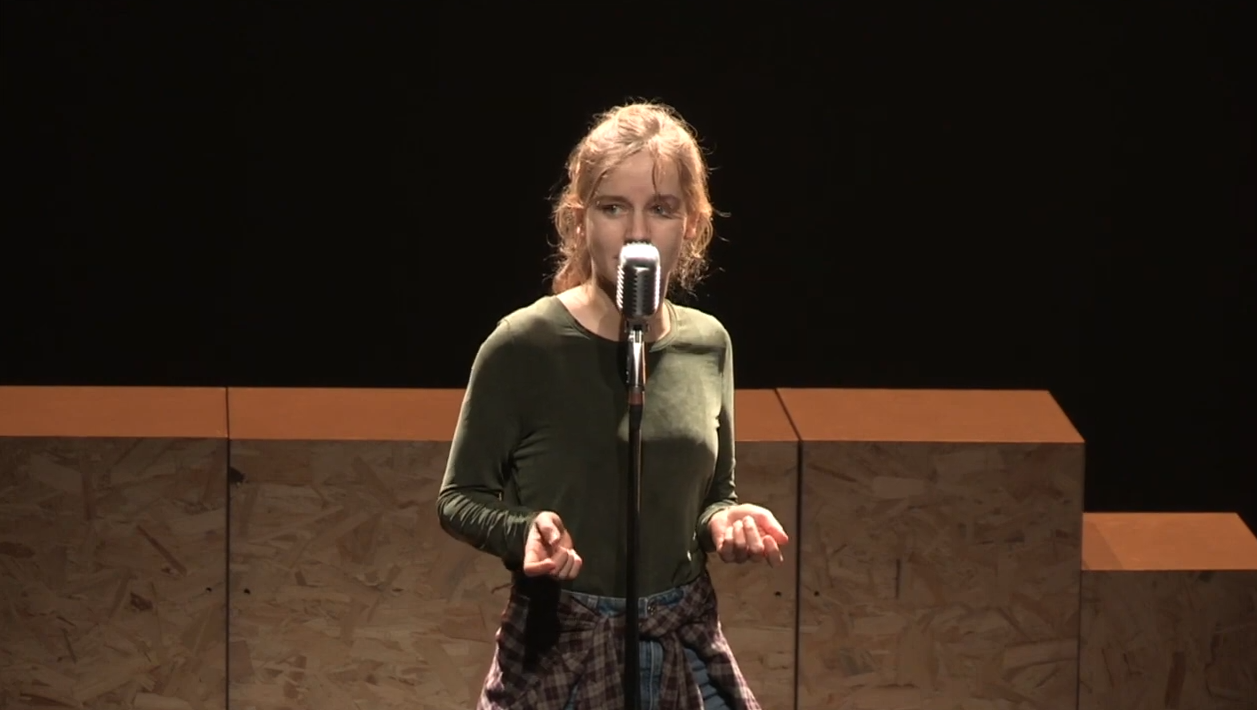
\includegraphics[width=17cm,height=9.601cm]{../assets/Pictures/10000201000004E9000002C6AB55B1C7B6546AEF.png}
\caption{Pig Boy par Théâtres de l\textquotesingle Entre-Deux, première partie}\label{fig:fig-1-1}
\end{figure}

\begin{figure}
\centering
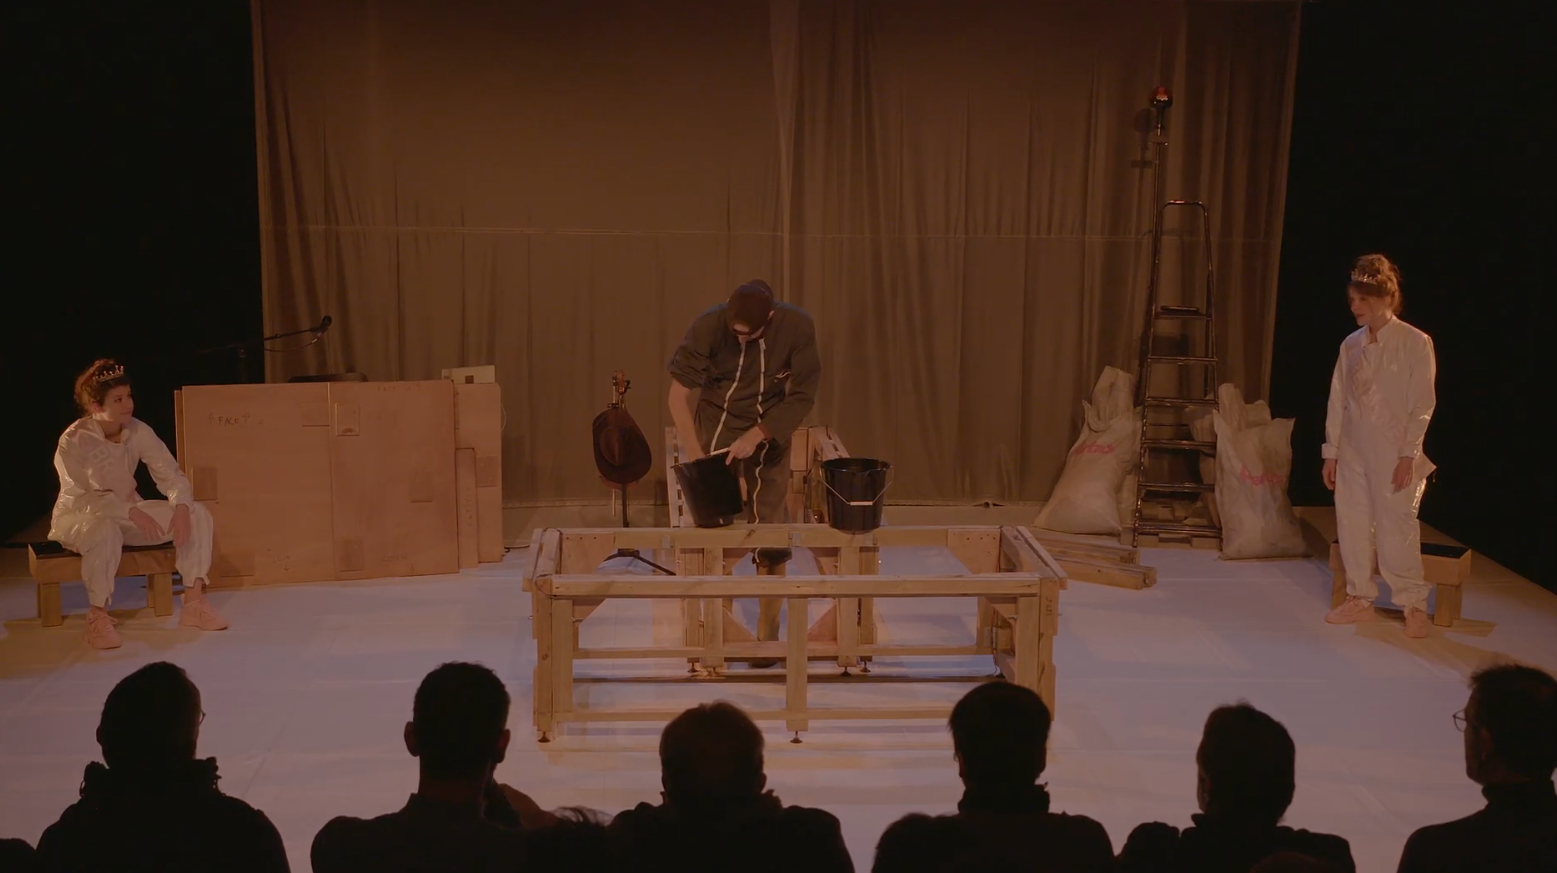
\includegraphics[width=17cm,height=9.532cm]{../assets/Pictures/100002010000061500000369BC796E070B503D8D.png}
\caption{Pig Boy par Le Bruit des Cloches, première partie}\label{fig:fig-1-2}
\end{figure}

Pour la partie 2, seul Théâtres de l'Entre-Deux décide de donner une existence au porc-star dont on fait le procès~: un des comédiens, partiellement bandé de tissu blanc, incorpore Pig Boy de façon assez animale, réagissant aux stimuli de la salle et des autres interprètes, regardant avec attention autour de lui mais semblant être perdu dans cette salle (figure~\ref{fig:fig-1-3}). À la fin du procès, il est habillé pour son exécution, comme l'indique le texte. Les interprètes du Bruit des Cloches situent Pig Boy devant elles, à peu près au milieu du public et regardent dans cette direction lorsque la parole est à lui. Sa corporéité est donc laissée à l'imagination des spectateurices, et elle est très libre puisque Pig Boy n'émet même pas de sons qui pourraient renvoyer à son statut de cochon. Dans la mise en scène de Détour 21, toutes les interventions sont coupées, et là encore le discours qui est tenu sur Pig Boy est exclusivement indirect.

\begin{figure}
\centering
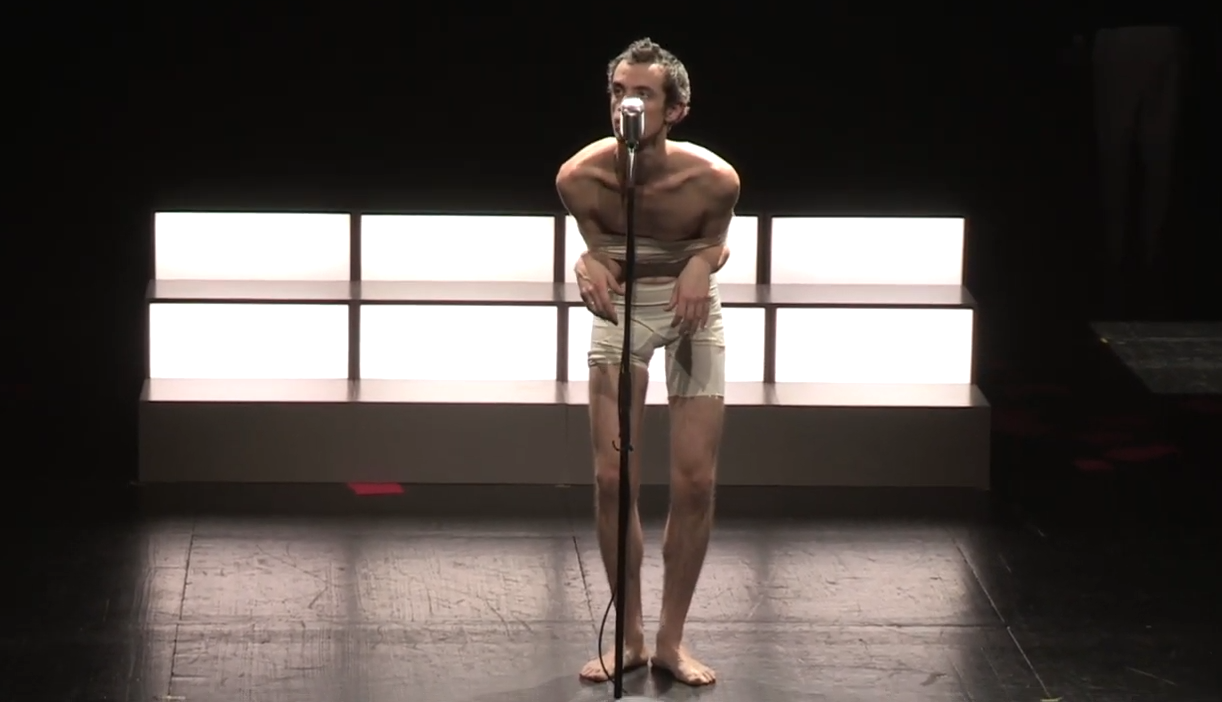
\includegraphics[width=17cm,height=9.767cm]{../assets/Pictures/10000201000004C6000002BEFCEC39B4E0EBE82E.png}
\caption{Pig Boy par Théâtres de l\textquotesingle Entre-Deux, deuxième partie}\label{fig:fig-1-3}
\end{figure}

Pour la troisième partie, bien que l'expression \emph{Pig Boy} renvoie plutôt aux petits de la truie, c'est plutôt cette dernière, de qui le discours émane, qui est incarnée par les comédien·nes. Le texte peut laisser penser que la truie est l'origine de cette nouvelle espèce et en fait déjà partie, puisque c'est porter des petits hybrides qui l'a métamorphosée et rapprochée des humain·es, en lui donnant la faculté de penser. La mise en scène de la compagnie Théâtres de l'Entre-Deux, là encore, décide de faire jouer les personnages chimères par des interprètes humaines, en chargeant le jeu des acteurices d'une qualité animale (). Ce sont les trois actrices de l'équipe qui portent le texte de la troisième partie~: leurs blouses de papier renvoient à l'univers médical et clinique humain, on peut par exemple y reconnaître les blouses des maternités~; cependant leurs corps sont mus dans une gestuelle peu humaine, leurs positions arquées, leur démarche difficile. Elles portent à la fois l'incarnation de la truie telle qu'elle est décrite dans le texte, et charrient avec elles l'imaginaire d'humain·es -- de femmes -- dans un milieu clinique, l'association des deux provoquant l'apparition d'un troisième univers fantasmé à la frontière des deux, des humain·es traité·es comme des animaux de laboratoire. L'aspect chimérique est traduit par cet entre-deux, où on ne sait pas bien ce que le personnage de la pièce a d'humain et d'animal. Le metteur en scène Philippe Mangenot m'a également fait part d'une piste de travail pendant la création, qui liait les trois interprètes dans un seul et même vêtement, comme un même corps, renforçant l'unité de ce personnage malgré les trois voix qui portent son texte. Cette piste n'a finalement pas été gardée pour la mise en scène finale (peut-être parce que l'hybridation du personnage était mieux transmise par la superposition des deux univers décrits au dessus que par la visualisation d'une chimère à trois têtes), mais on peut retrouver cette unité dans la similarité de leurs états de corps respectifs et dans leur marche synchrone par exemple. Le Bruit des Cloches, comme pour la première partie, sépare le texte de la truie de son incarnation. Une quatrième interprète, que l'on n'a pas vue dans le reste du spectacle (elle est collaboratrice artistique et coordinatrice du projet), joue la truie, une bête au corps de femme, à la peau d'argile et à la tête de cochon, chimère à mi-chemin. Un effet de lumière rend son apparition saisissante~: un flash de lumière froide, très court et proche de la bête, suivi tout de suite d'un retour dans le noir (). À cette vision d'horreur répond directement le premier mot du texte~: «~Vu.~» (p.55). Le parcours de l'interprète retrace celui du personnage du texte~: elle commence enfermée dans un box étroit, une flaque d'un liquide sombre dont on ne sait si c'est du sang, de la boue ou de la fiente près d'elle, et parvient péniblement à s'extraire de cet espace pour entamer une progression lente qui l'amène à se relever sur ses deux jambes (). Ici, le texte n'est plus adressé au personnage incarné, mais est une émanation de sa pensée. On entend le monologue intérieur de la truie que l'on voit, et on comprend très vite qu'il s'agit de sa pensée puisque le masque ne parle pas. Le collectif Détour 21, ayant également pris le parti d'une harmonie de mise en scène des trois parties, décide de ne pas montrer le corps de la truie, mais plutôt de donner à voir ce qu'elle perçoit pendant sa fuite, par l'intermédiaire de courtes séquences vidéo sans son (vidéo 1). Le point de vue subjectif permet d'entrer dans les sensations du personnage, tout en laissant planer le doute sur sa nature physique. Cette indétermination est aussi présente dans le texte, qui commence directement à l'intérieur de la tête du personnage, si bien qu'au début on ne sait pas exactement \emph{qui }pense, et tout au long de la partie on n'a accès à la précision du personnage qu'au travers de ses sensations et sa perception du monde qui l'entoure.

\begin{figure}
\centering
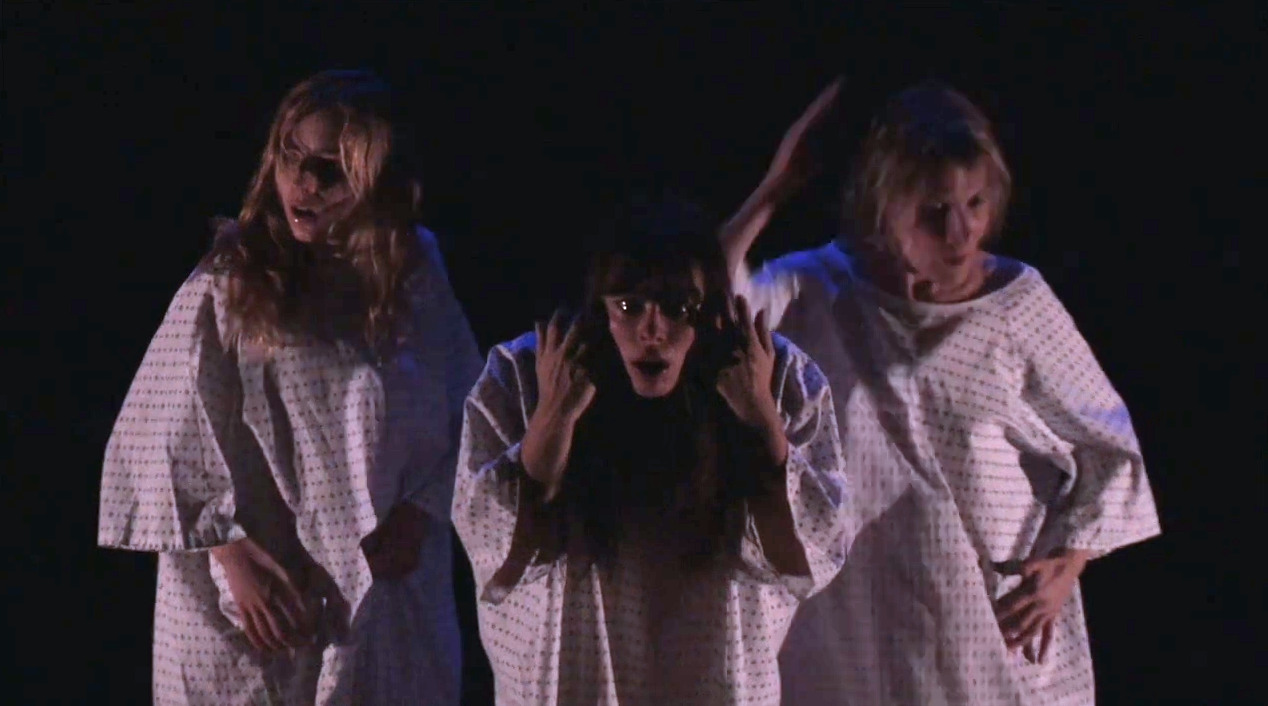
\includegraphics[width=17cm,height=9.463cm]{../assets/Pictures/10000201000004F4000002C2B712E44AAF95EAF0.png}
\caption{Truies par Théâtres de l\textquotesingle Entre-Deux, troisième partie}\label{fig:fig-1-4}
\end{figure}

\begin{figure}
\centering
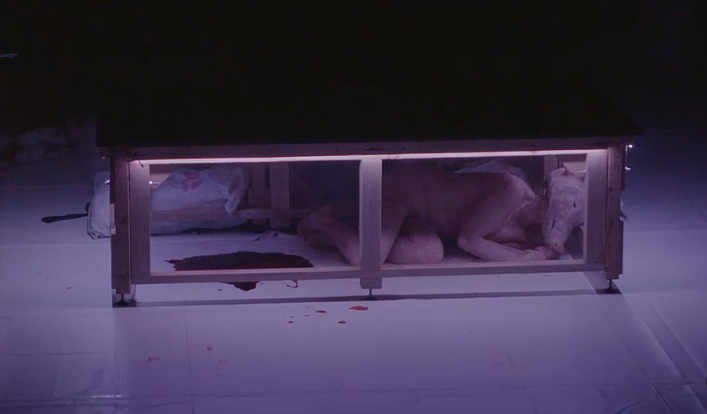
\includegraphics[width=16.887cm,height=9.888cm]{../assets/Pictures/10000201000002C30000019E3152FCACF0A1D307.png}
\caption{Truie par Le Bruit des Cloches, troisième partie (début)}\label{fig:fig-1-5}
\end{figure}

\begin{figure}
\centering
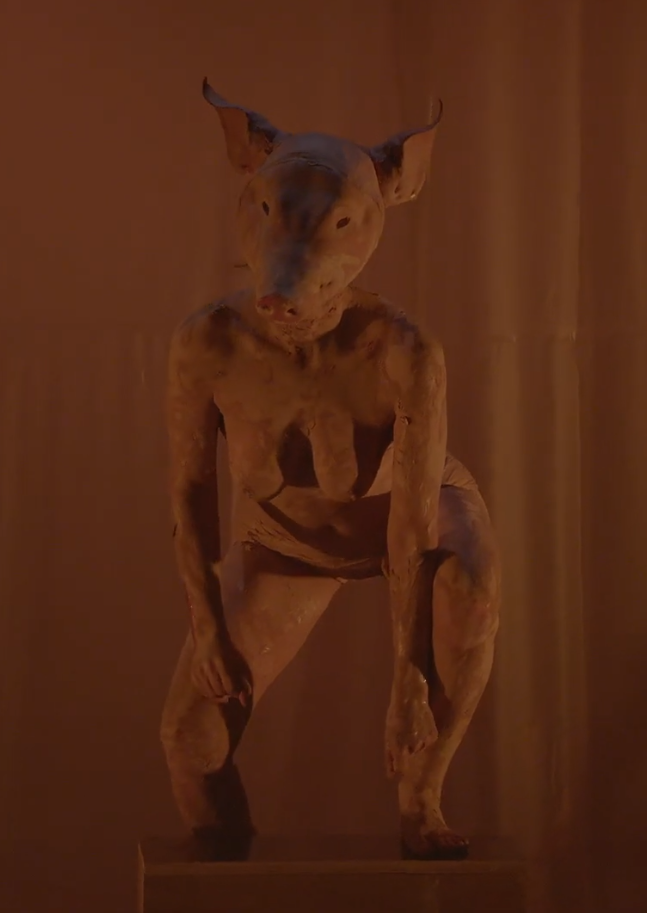
\includegraphics[width=10.555cm,height=14.891cm]{../assets/Pictures/100002010000028700000391A91BA4932910F52F.png}
\caption{Truie par Le Bruit des Cloches, troisième partie (fin)}\label{fig:fig-1-6}
\end{figure}

\phantomsection\label{video-1}
{vidéo 1.} Détour 21, extrait de travail pour les séquences video de la troisième partie. Réalisation par Léo Garcia - Telegraph prod

Paul Deharme écrivait en 1930 que l'absence de visuel fait marcher l'imaginaire, et que quand il y a visuel, les arts qui utilisent ce sens sont souvent obligés de correspondre aux images mentales préexistantes que se font les spectateurices.{[}@pauldeharmePourArtRadiophonique1930, p.~32{]} Effectivement, on peut constater que certains choix d'incarnation des mises en scène répondent à des codes de représentation pré-établis qui permettent aux spectateurices de reconnaître rapidement ce dont on leur parle (ils·elles reconnaissent plus qu'ils·elles ne voient)~: dans la première partie de Théâtres de l'Entre-Deux par exemple, Mathilde -- dont le héros est amoureux -- est incarnée par une jeune femme blanche, blonde et mince. Je prends cet exemple parce qu'il résonne avec celui que donne Deharme de l'impossibilité de représenter une Yseult «~laide~»{[}@pauldeharmePourArtRadiophonique1930, p.~32{]}~: les codes de représentation semblent plus difficiles à subvertir lorsqu'il s'agit du contrôle des corps féminins. Cependant, on peut également remarquer des contre-exemples, ce qui tempère l'affirmation de Deharme. Dans la même partie de la même mise en scène, les \emph{miss} du jeu télévisé sont incarnées une fois, lors de leur première occurrence dans le texte~: ce sont deux hommes en caleçon noir, ayant des corps très différents l'un de l'autre, qui montent sur le podium afin d'être jugés de haut en bas par le père du héros. Le théâtre n'est peut-être pas autant soumis à l'injonction au visuel, si tant est qu'il soit même considéré comme un art visuel. Une autre particularité, qu'on trouve plus régulièrement au théâtre qu'à la radio et que soulève également Deharme, est qu'au théâtre les représentations mentales que se font les spectateurices se calquent sur les représentations physiques qui leur sont données à voir. À la radio, il est difficile de maintenir des images mentales fixes qui ne fluctuent pas au gré de l'histoire, elles peuvent être chavirées par les sensations à tout instant.{[}@pauldeharmePourArtRadiophonique1930, p.~37{]} Mais n'est-ce pas un avantage dans le cas des personnages de chimères, qui peuvent ainsi être sans cesse réimaginés à mesure que le texte se précise~? Pourquoi «~suppléer à l'absence de vision, \emph{au lieu de chercher à s'en servir}~»~?{[}@pauldeharmePourArtRadiophonique1930, p.~19{]}

Il serait hâtif de considérer la radio comme un médium dépourvu de toute matérialité. «~Privée de visage, {[}\ldots{]} de mains et de corps, la voix de celui qui parle au micro n'est pas désincarnée~» disait Jacques Copeau en 1951.\footnote{Cité dans {[}@marionchenetier-alevTheatreRadio{]}.} Dans la création radiophonique de \emph{Pig Boy 1986-2358}, on peut relever quelques exemples de voix qui charrient un corps plus ou moins précis~: penchons nous sur les accents. Dans la deuxième partie, la présidente Shanon -- joué par Rose Martine, comédienne franco-haïtienne -- a un accent ténu mais suffisant pour faire apparaître à l'esprit des auditeurices l'image mentale d'une personne noire (et selon la capacité de l'auditeurice à distinguer les accents, une personne antillaise, ou même une personne haïtienne). De la même manière, la voix de Katsue Matumato -- interprétée par Yilin Yang, actrice taïwanaise -- indique son origine asiatique, qui est également explicite dans le texte (le personnage est japonais). Les mises en scène ne se sont pas risquées à reproduire l'accent de Katsue, ce qui aurait posé un certain problème de représentation sur scène des personnes racisées, mais proposent plus volontiers des accents régionaux pour les personnages français. Le transliver vlak.gogo, boucher à Quimperlé, a par exemple un accent prononcé dans la mise en scène du Bruit des Cloches, un accent qui évoque d'ailleurs plutôt le Sud que la Bretagne (le collectif étant lui-même basé à Clermond-Ferrand), mettant ainsi sur un même plan les accents régionaux sans s'approprier une parole étrangère. Ce même collectif décide cependant d'interpréter Tao Wong comme un personnage s'exprimant dans sa langue maternelle et traduit par la présentatrice. Formellement, c'est une idée très astucieuse car elle permet un régime de discours très courant dans les médias radiophoniques et télévisés et sur internet, celui de paroles venues de loin pour apporter leur expertise et traduites en direct, illustrant ainsi la mondialisation et correspondant à l'aspect international du translive. Elle permet aussi de donner une certaine forme de crédibilité au scientifique, qu'on respecte tant il a l'air convaincant dans sa propre langue. Cependant, je me dois de remarquer que cette incarnation a plutôt tendance à faire rire la salle et à rendre le personnage ridicule, teintant légèrement le passage d'une connotation raciste, et pose encore une fois la question de la représentation des personnes étrangères dans le scène du théâtre français et de la nécessité de jouer «~à la place de~». En l'occurrence, ce passage ne rend même pas la pièce particulièrement représentative ou accessible pour les locuteurices du chinois puisque qu'il ne s'agit pas de cette langue mais d'un grommelot inspiré. La radio, parce qu'elle ne présente que les voix, ne souffre pas du potentiel décalage entre la voix et le corps qui la porte. L'auditeurice suppose la voix réelle, attachée au corps qui lui correspond dans l'image mentale qu'il·elle s'en fait. De fait, les conditions de production des œuvres radiophoniques permettent de présenter beaucoup plus de voix différentes dans une heure d'émission que ne pourrait le faire le théâtre en une heure de spectacle. Pour la deuxième partie de \emph{Pig Boy}, cette possibilité est un atout puisque les personnages sont extrêmement nombreux, ce qui pousse les comédien·nes des différentes mises en scène à en incarner beaucoup. Néanmoins, on voit avec l'exemple de Yilin Yang qui joue une japonaise et que l'on suppose donc par défaut japonaise, mais qui est en fait taïwanaise, que la vérification de l'origine des voix ne donne pas toujours raison à la radio et que des enjeux symboliques et économiques de représentativité dans le milieu peuvent aussi se poser.

\subsubsection{Espaces de jeu, espaces de son}\label{espaces-de-jeu-espaces-de-son}

Les trois mises en scène que j'ai étudiées sont des dispositifs frontaux, disposant d'une scénographie adaptée aux trois parties de la pièce. Une des particularités de la mise en scène de Détour 21 est la présence d'un écran de diffusion, qui crée donc un espace de projection en plus de la surface de jeu du plateau. Lors de la deuxième partie, de nombreux espaces spatio-temporels se côtoient dans le texte. Il y a l'espace de l'émission en direct, dans lequel se trouvent le·la présentateurice et l'audience de l'émission («~il est 20h02 Nous sommes en live depuis San Francisco, California~» p.21)~; les translivers, qui sont chacun·e dans des espaces différents, mais qui sont dans la même temporalité que le direct («~Hey~! Salut salut.~» p.25)~; enfin, les épisodes qu'on pourrait qualifier de \emph{prêt-à-diffuser}, qui sont les séquences de reportage éditées qui reviennent sur des faits passés, les musiques, les messages de la plateforme et les jingles, qui présentent donc une temporalité d'enregistrement antérieure au présent du direct («~Depuis dix ans, il représente la marque PERTA, premier éleveur et fournisseur mondial de viande de porc~» p.21). Pour figurer ces espaces et les différencier, les mises en scène séparent également leur espace de jeu. Dans la mise en scène de Détour 21, celle qui est le plus rigoureuse sur les changements d'espace, les passages de direct se situent à l'avant scène, où se trouve la présentatrice, et tous les personnages qui prennent la parole en direct font systématiquement le chemin du fond de scène à l'avant scène, tout en enfilant un micro-casque accessoire, figurant ainsi leur entrée dans l'espace de parole en direct. Les commentaires des translivers ainsi que les SMS se trouvent affichés à l'écran, renforçant la médiatisation d'une parole très éloigné spatialement du lieu de l'action. Enfin, tous les prêts-à-diffuser sont interprétés par trois des comédien·nes en fond de scène, à la manière d'automates qui incarnent les différentes paroles des personnages selon les besoins, puis retournent à une neutralité robotique. L'agencement de Théâtres de l'Entre-Deux pose aussi le direct à l'avant de la scène, où se trouvent quasiment tout du long le personnage de la présidente Shanon et l'interprète qui prend le rôle de la narratrice (deux femmes en alternance). Les commentaires se font à l'arrière scène, dans des espaces rectangulaires délimités par la lumière. Pour ce qui est des prêts-à-diffuser, ils sont interprétés par les acteurices, sur différents endroits du plateau selon les besoins, mais sont toujours suivis par une création lumière qui rend les espaces clairs. Pour la mise en scène du Bruit des Cloches, le direct et les prêts-à-diffuser se partagent l'espace de jeu~: les comédiennes n'étant que deux à porter le texte, certaines délimitations sont adaptées pour que les espaces se suivent plus naturellement. L'espace des commentaires est lui figuré par un accessoire regardé par l'interprète qui porte le commentaire assise dans un coin. Cet accessoire produit une lumière très froide projetée sur le visage de le·la commentateurice, comme le ferait un écran de portable. Cet espace lumineux permet de figurer clairement le type de consommation très solitaire que les translivers peuvent avoir de l'émission, chacun·e confiné·e dans son espace. Il est aussi intéressant de remarquer que le passage du rappel des faits se joue dans le noir dans cette mise en scène, ce qui permet à la fois de produire l'atmosphère angoissante spécifique aux émissions d'enquête, mais aussi d'être très précis sur les paroles d'incises, qui sont figurées à la lampe torche~: maîtriser la lumière, c'est maîtriser ce qui est montré.

La création radiophonique tient compte elle aussi des différents espaces proposés par la deuxième partie du texte, même si elle n'utilise que le son pour les figurer. Le présentateur et les téléspectateurices de l'émission ont été enregistrés ensemble, dans une petite salle de cinéma de l'espace Cardin à Paris (Radio France était en travaux au moment de la création de la pièce, en 2019). Cette technique d'enregistrement «~réaliste~», assez courante dans les fictions produites par France Culture, découle essentiellement de nécessités de production, car le temps de post-production est très limité donc les gains de temps qui peuvent être faits à l'enregistrement sont maximisés. Dans cet exemple, les auditeurices perçoivent immédiatement l'espace de l'émission comme une salle, de par son acoustique et sa réponse fréquentielle, alors même que le traitement et les effets posés sur les voix en post-production sont minimes. De la même façon, les commentaires des translivers et les incises des prêts-à-diffuser sont enregistrés en conditions réelles, dans des espaces différents et avec des micros de portable, ce qui rend très réalistes les prises de paroles des utilisateurices «~là où ils·elles sont~»~: son des environnements dans lesquels ils·elles se trouvent (rue, appartement, intérieur, local professionnel), la qualité des appareils utilisés pour communiquer (portable, micro d'ordinateur, micro et carte son). Tous ces éléments, aussi minimes soient-ils, enclenchent notre écoute causale et nous fournissent de nombreuses informations sur le type de parole auquel on a affaire (parole institutionnelle ou non, statut économique et position de classe de l'utilisateurice\ldots). Prenons par exemple la parole de Maxime Guimarch, qui est très propre, prise de près, sans bruits parasites et sans indication d'espace si ce n'est, en creux, la qualité de son matériel qui doit être onéreux (audio 1). Sa parole est comme aseptisée, débarrassée de tous les éléments qui pourraient donner des informations sur le lieu où la prise de parole à lieu~; bien sûr, cette absence d'informations est une information. Si on prend au contraire l'incise page 22 «~He inspired me for my new collection~», le bruit ambiant est si fort qu'il masque progressivement la parole de l'interviewé, jusqu'à ce que l'incise soit coupée à cause du bruit (audio 2). Cette comparaison de l'environnement sonore nous indique que les personnages qui parlent ne se trouvent pas aux mêmes endroits et n'ont pas le même statut, et cela contribue à préciser nos images mentales~; la création radiophonique ne laisse bien entendu aucun de ces éléments au hasard. Il y a également toutes sortes de réponses de salle dans les commentaires et les interventions qui se situent dans d'autres endroits que la salle de l'émission. Ces réponses fréquentielles peuvent être prises à l'enregistrement, être exagérées avec un traitement à l'égaliseur multibandes ou même émulées synthétiquement comme le serait un effet de \emph{reverb} classique. Parmi les plus remarquables, celle de la transliver Truelove\_Austria.(audio 3) Contrairement aux mises en scène, la création radiophonique ne place aucun personnage avec le·la présentateurice, si ce n'est le public de l'émission, et situe toutes les paroles directes du procès, c'est-à-dire dans la même temporalité, sur un pied d'égalité~: les membres de la cour, les témoins comme Katsue Matumato et Maxime Guimarch, les translivers, tous·tes sont encadré·es par une tonalité assez caractéristique -- le son d'allumage du Nagra -- et l'expression «~on air~» qui qualifie dans le monde anglophone ce qui est diffusé à la radio ou la télévision. Ainsi, on imagine la Présidente Shanon, Tao Wong, vlak.gogo et tous·tes les autres translivers chacun dans un espace singulier et personnel, et l'espace du·de la présentateurice comme «~une immense cabine de régie~» (selon l'expression de Christophe Hocké). Une précision qui permet d'ancrer l'espace du direct dans notre imaginaire commun est l'utilisation des filtres par l'équipe de réalisation, qui permet de faire entendre des translivers non seulement diffusés à nous comme si nous étions translivers (le régime d'écoute de base, qui ne contient que l'enregistrement du personnage qui parle), mais aussi diffusés dans les espaces de l'histoire (la salle des téléspectateurices, les différents espaces dans lesquels se trouvent chacun des personnages\ldots), ce qui déplace l'auditeurice aux différents endroits d'écoute possible, et lui donne ainsi une sensation plus omnisciente que celle du simple transliver. Par exemple, les accusateurices tirées au sort ont environ quatre secondes de parole lors de leur nomination, et nous passons ces quatre secondes chez elleux~: les auditeurices de la création sonore l'identifient tout de suite car l'enregistrement fait entendre l'émission filtrée par la source de diffusion de l'accusateurice (en l'occurrence les applaudissements des téléspectateurices, par le son d'une télévision ou d'un ordinateur) et la voix beaucoup plus proche des accusateurices qui réalisent leur nomination dans un espace qui est vraisemblalement leur maison (bruits de couverts, présence d'un·e conjoint·e\ldots). De la même manière, on entend Tao Wong qui s'apprête à prendre la parole chez la Présidente Shanon, vlak.gogo en salle, il y a également pendant le discours de Maxime Guimarch des allers-retours entre l'enregistrement du personnage, sa réception en salle et la réception de la salle chez lui. Ce procédé renforce ainsi le réalisme de l'interface, ou chacun·e est devant son écran, tout en donnant accès aux auditeurices aux différents espaces de l'histoire.

audio 1

\phantomsection\label{audio-1}

audio 2

\phantomsection\label{audio-2}

audio 3

\phantomsection\label{audio-3}

Notons qu'au suicide de Maître Spare, la réaction commune des téléspectateurices et des translivers en une vague de suicides en direct, et la tentative de la chaîne Nation News de réguler le flux violent en proposant une page de publicité, tendent à brouiller les différents espaces. Dans la création radiophonique, l'apparition d'une musique que l'on suppose pour la première fois dans la deuxième partie extra-diégétique vient déjà interroger les auditeurices sur l'espace d'écoute présenté (à 36:11) (audio 4). Une intervention de transliver particulièrement hachée vient distordre d'autant plus l'espace (entre 36:49 et 36:56), puis une montée progressive de commentaires amène une sorte de grand \emph{bug} (37:20 - 37:55) où tous les espaces se mélangent, les artefacts de connexion ou \emph{lags} se multiplient (distorsion de la parole, erreurs de temporalité dans la continuité de la parole qui ressemblent à un disque qui saute\ldots) jusqu'à la reprise de contrôle complète de l'interface PERTA. Les mises en scène opèrent selon un procédé similaire, où elles trépassent les conventions spatiales qu'elles ont posées tout au long de la deuxième partie pour créer une sensation de flou et de submersion de l'émission.

audio 4

\phantomsection\label{audio-4}

\subsubsection{Montrer ou faire entendre}\label{montrer-ou-faire-entendre}

Le monologue de Maxime Guimarch propose un cas intéressant dans lequel le théâtre doit faire le choix de dire ou de montrer (et la radio de dire ou ne pas dire, à défaut de montrer)~: tout au long de la réplique se trouvent entre crochets des propositions, dont on comprend qu'elles se réfèrent à des imaginaires visuels. «~{[}mer turquoise -- quatre enfants -- une glace coule pistache sur des doigts bronzés{]}~» (p.41) ou encore «~{[}logo -- marque déposée{]}~» (p.41) sont des ensembles qui servent à décrire des images. De là peuvent être faites deux propositions~: dire le texte ou montrer les images. La voie de la monstration d'images à l'avantage d'ancrer le monologue de Maxime Guimarch dans l'exercice de style assez spécifique de la présentation \emph{powerpoint}, exposé ponctué d'appuis visuels diffusés par l'orateurice, et qui correspond bien à l'imaginaire du chef d'entreprise capitaliste. Comme il le ferait lors d'une réunion avec les promoteurices, actionnaires et autres partenaires de son entreprise, Maxime Guimarch vend sa marque, son produit, sa personne aussi. Seul le collectif Détour 21 décide de se prêter à cet exercice. L'autre possibilité est de dire le texte entre crochets, un parti que prennent Théâtres de l'Entre-Deux et Le Bruit des Cloches. Théâtres de l'Entre-Deux utilise un signal sonore qui rappelle le changement de diapositive (produit avec des baguettes sur scène) pour indiquer l'apparition d'une image, que les interprètes situent sur un écran imaginaire au dessus du public -- donc devant eux -- image qui est ensuite décrite par une interprète avec les mots entre crochets. Le Bruit des Cloches procède un peu de la même manière, à la différence près que l'écran imaginaire est situé en fond de scène -- derrière Maxime Guimarch -- et qu'il n'y a pas de son associé au changement d'image. Philippe Mangenot m'a confié à ce sujet qu'il trouvait le choix des mots entre crochets drôle et très parlant de lui-même, et que ne pas faire profiter les spectateurices de cette partie de l'écriture était à son sens dommage. De plus, il considère que même les meilleures images qu'il pourrait trouver pour représenter les propositions écrites seront moins puissantes si elles sont imposées aux spectateurices que la suggestion d'images mentales que les mots provoquent à la lecture. Il est vrai que la parole et la lecture ont le point commun de ne pas imposer de visuel, comme nous l'avons déjà dit dans ce mémoire. Elles créent des images mentales, et l'intention de ne pas forger d'images mais de laisser faire les imaginaires est bonne. Cependant ici, le cadre de l'émission, les différents personnages et Maxime Guimarch lui-même ont des existences visuelles, et le·la spectateurice navigue dans un monde d'images. Les images mentales que les mots peuvent créer ne sont donc pas isolées du reste des représentations visuelles du spectacle, et risquent d'être imprégnées par ces dernières. Par ailleurs, les actions de lire et dire sont fondamentalement séparées par le sens par lequel elles passent. Alors que les mots, comme symboles visuels, transportent uniquement leur forme graphique quand ils arrivent à notre conscience, les mots dits passent par l'ouïe et charrient donc avec eux la sensation sonore qu'on en a. La sonorisation de mots censés ne provoquer que des images mentales et non des sensations sonores (on suppose ici que l'autrice du texte n'a choisi ces mots que pour leur justesse dans la production d'images mentales et pas pour leurs sonorités) pose question~: la voix est-elle vraiment le meilleur médium pour transmettre des images mentales~? Dans la création radiophonique, médium qui n'impose pas non plus d'images visuelles, ces propositions entre crochets ont finalement été coupées, seule la parole de Maxime Guimarch est entendue.

Une réflexion de Christophe Hocké me revient~: à propos de la deuxième partie, il disait qu'il avait comme intention une esthétique kitsch, dans le pastiche des contenus internet qui n'utilisent que des images et des sons libres de droit, du domaine public ou de stocks \emph{open source}. D'abord contrainte par des raisons économiques, cette esthétique s'est ensuite répandue sur internet pour devenir caractéristique de certains contenus. Les propositions de Gwendoline Soublin pour les images qui ponctuent le discours de Maxime Guimarch sont écrites très succinctement, et font penser aux mots-clefs qu'on peut donner aux intelligences artificielles~: peut-être une piste est à creuser du côté des images que ces propositions pourraient générer. Ici deux exemples générés à l'aide de l'IA de ChatGPT (figure~\ref{fig:fig-1-7}) et de Canva (figure~\ref{fig:fig-1-8}).

\begin{figure}
\centering
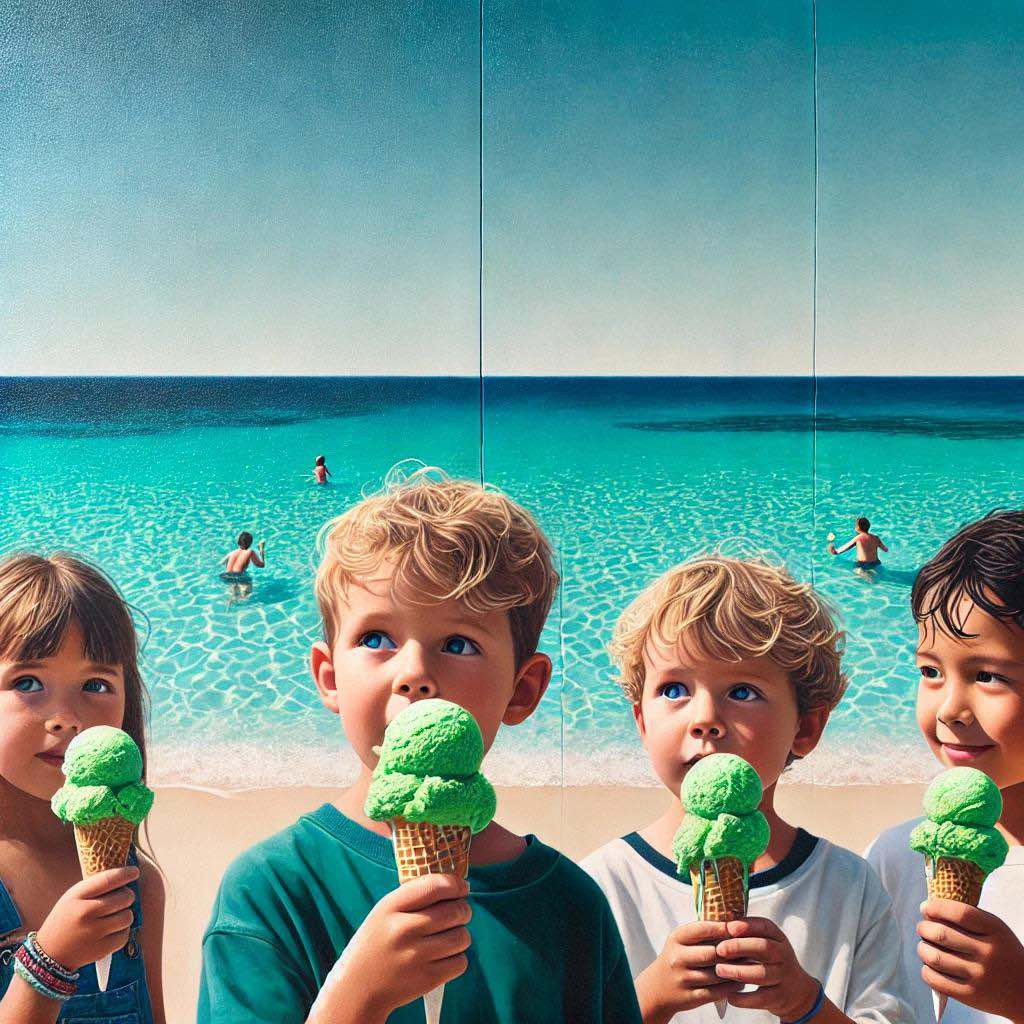
\includegraphics[width=17cm,height=17cm]{../assets/Pictures/1000000000000400000004005745ADB05D1DDF55.jpg}
\caption{{[}mer turquoise -- quatre enfants -- une glace coule pistache sur des doigts bronzés{]} dans ChatGPT}\label{fig:fig-1-7}
\end{figure}

\begin{figure}
\centering
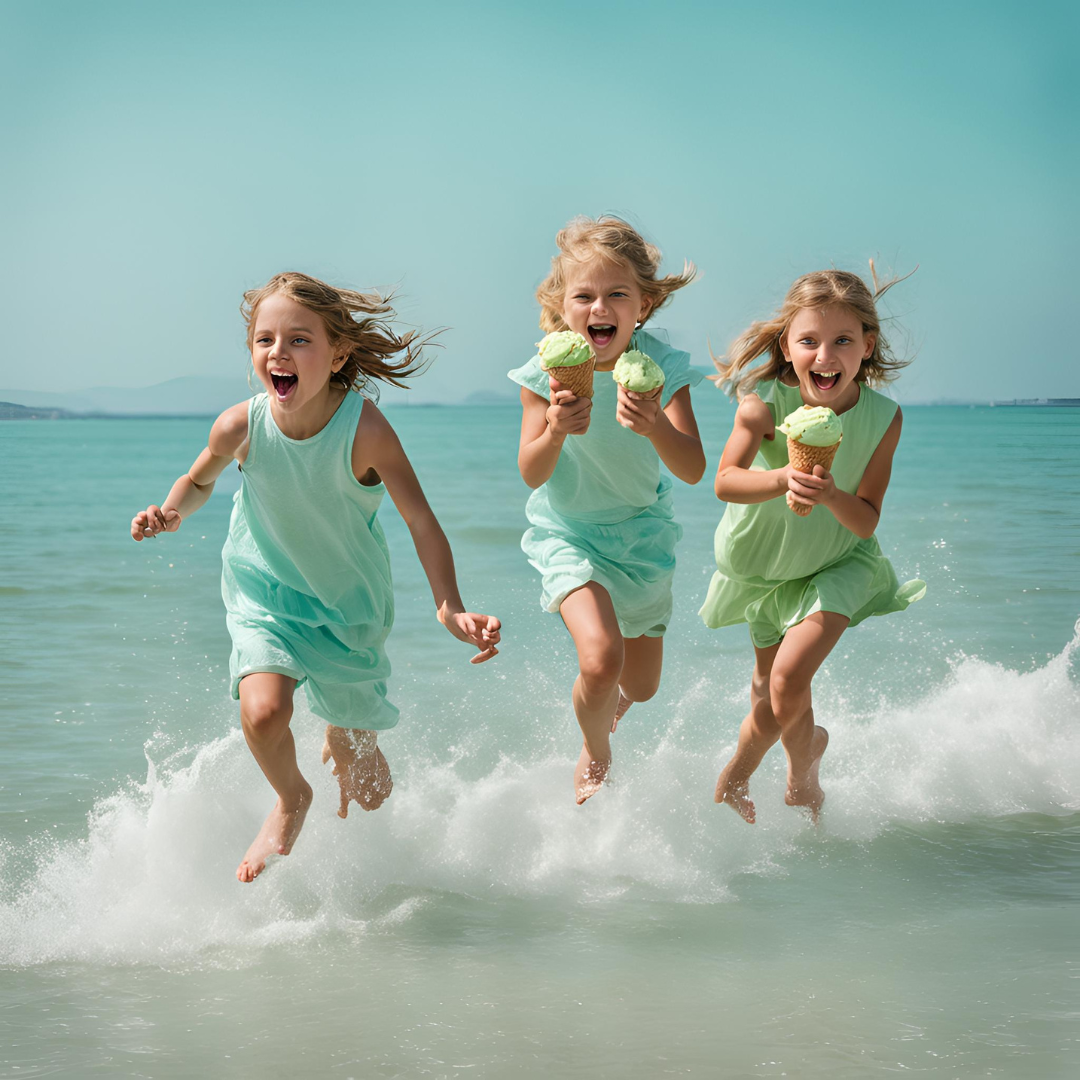
\includegraphics[width=17cm,height=17cm]{../assets/Pictures/100002010000043800000438C6D70231BDF286FC.png}
\caption{{[}mer turquoise -- quatre enfants -- une glace coule pistache sur des doigts bronzés{]} dans Canva}\label{fig:fig-1-8}
\end{figure}

\subsection{Acoustique ou Amplifié~? Les micros et la voix}\label{acoustique-ou-amplifiuxe9-les-micros-et-la-voix}

À la radio comme au théâtre, la question de l'amplification se pose. La voix de radio nécessite une médiation, par l'enregistrement, aussi la question de l'amplification désigne plus volontiers les questions de transparence des microphones utilisés et de \emph{re-amplification }(technique d'enregistrement qui permet de faire entendre différentes couleurs d'espaces et de micros). En ce qui concerne le théâtre, les voix sont traditionnellement acoustiques, mais l'arrivée progressive des techniques d'enregistrement et d'amplification a aussi permis de repenser les voix théâtrales avec ces nouveaux outils. Les microphones, en tant qu'objets matériels, peuvent être cachés ou à vue selon les cas. Lorsqu'ils sont visibles, ils soulèvent la question de leur mise en scène et en jeu. Enfin, la voix amplifiée porte en creux la question de sa temporalité~: est-ce une voix en direct, est-ce une voix différée, est-ce une voix pré-enregistrée et modifiée~? Dans la pièce \emph{Pig Boy 1986-2358}, et notamment dans la deuxième partie, l'écriture de l'autrice condense des temporalités différentes (direct spatio-temporel, direct temporel, différé) et les accole sans transition, les enchaîne de manière à les lier entre elles et ainsi créer, paradoxalement, une unité d'action.{[}@rudolfarnheimRadio2005, p.118{]} Cela engage les différentes mises en scène et la mise en ondes à se demander comment montrer cette émission qui se situe dans un univers médiatique d'une part, et comment réinvestir les codes visuels et sonores de cet univers dans les voix de manière à pouvoir intégrer les personnages dedans d'autre part. Dans cette partie, nous regarderons de plus près comment les trois mises en scène et la création radiophonique traitent ces enjeux de voix et d'amplification.

\subsubsection{Le jeu de l'acoustique au théâtre}\label{le-jeu-de-lacoustique-au-thuxe9uxe2tre}

Le théâtre est un art qui privilégie traditionnellement la voix acoustique des acteurices. En témoignent l'architecture des théâtres anciens aux acoustiques facilitant les prises de parole, et la relative jeunesse des techniques d'amplification électriques. Philippe Mangenot dit humoristiquement s'attacher au théâtre «~archaïque~» pour renvoyer à son choix de ne pas mettre de vidéo ni de texte pré-enregistré dans sa mise en scène. En effet, le spectacle de Théâtres de l'Entre-Deux n'a recours qu'à la diffusion de la musique. L'intégralité du texte gardé -- il y a quelques coupes, peu nombreuses cependant -- est dit en direct par les comédien·nes, la majorité du temps avec des micros -- nous y reviendront ensuite. Si nous nous concentrons uniquement sur le débit des acteurices et pas sur le traitement des voix, nous pouvons observer des tentatives de pastiche des codes formels de la voix des médias par la parole immédiate. En deuxième partie par exemple, le jingle de l'émission \emph{Procès} est fait en direct~: le mot Procès est répété par les différent·es interprètes et spatialisé aux quatre coins de la scène, reproduisant ainsi un code de présentation radiophonique. La création radiophonique utilise d'ailleurs elle aussi ce procédé pour le jingle de \emph{Procès} mais aussi de \emph{Nation News} ou encore de la \emph{Révélation}. Autre exemple, la voix qui énonce les mesures de prévention pour le rappel des faits («~Cette séquence est interdite aux moins de 16 ans, aux femmes enceintes ainsi qu'aux personnes transplantées pour des raisons évidentes de décalage dismorphique et de trouble émotionnel cathartique.~» p.23) imite le débit extrêmement rapide et articulé des voix optimisées pour passer le maximum d'informations le plus vite possible, qu'on trouve régulièrement à la télévision, pour lire du texte par ailleurs affiché, et dans la publicité plus généralement. Là encore, la mise en scène de Théâtres de l'Entre-Deux, du Bruit des Cloches et la création radiophonique s'accordent sur la référence du texte à ce débit et décident de le mettre en voix. Un deuxième effet de transformation du débit de voix acoustique pour correspondre aux codes des voix médiatisées est l'imitation des voix automatiques, à différencier des voix synthétiques, comme on peut encore en trouver dans les trains par exemple. À partir de mots enregistrés un à un, un système de lecture automatique reconstitue des phrases, donnant ce débit très haché et aux intonations incohérentes, hors du contexte syntaxique. Dans la mise en scène de Théâtres de l'Entre-Deux, les interprètes recréent cet effet pour le texte des SMS, en les disant de manière très segmentée, à deux voix qui alternent au milieu des phrases et selon les mots. Dans l'exemple qui suit, les mots en gras indiquent une voix différente~: «~Pensez-vous que \emph{\textbf{Pig Boy} }est un détraqué sexuel~? Répondez \textbf{\emph{OUI}} ou \textbf{\emph{NON}}. Do you think \textbf{\emph{Pig Boy}} is a sex addict~? Please answer \textbf{\emph{YES}} or \textbf{\emph{NO}}, please answer \textbf{\emph{YES}} or \textbf{\emph{NO}}, please answer \textbf{\emph{YES}} or\ldots{} (temps) \textbf{\emph{NO}}.~» (p.26). La répétition de la dernière phrase est ajoutée au texte original, créant un effet de \emph{lag}, accentué par l'effort que font les interprètes de répéter tous les mots avec les mêmes rythmes et intonations, la même «~musique~» (mots qu'utilisent les comédien·nes pour désigner un systématisme d'intonation, souvent perçu comme maladroit).

L'idée de pousser l'exactitude de l'intonation pour imiter ces voix que l'on entend toujours médiatisées semble judicieuse car un des éléments qui les caractérisent est leur reproductibilité, leur immuabilité. On \emph{re-connaît} un jingle parce qu'il est toujours le même, par définition. Peu importe ce qui le compose, il a été édité et mixé, il est désormais écrit sur un support -- numérique ou analogique -- et ni le texte, ni le son ne peuvent être modifiés. Un travail de la voix immédiate assez contre-intuitif doit être mené par les comédien·nes pour réussir à se fondre dans le débit de la voix automatique, qu'on reconnaît justement à sa froideur, à son aspect peu humain dans la mesure où même si le timbre de la voix est le nôtre, l'utilisation des mots qui est faite ne correspond pas aux règles de notre communication. Une «~musique~» apprise par cœur pourrait faciliter cette exécution, qu'il s'agisse de l'intonation ou du débit, souvent plus rapide que la voix humaine. Pour la mise en scène de Détour 21, nous travaillons encore à préciser ce travail vocal dans la deuxième partie. La première version des comédien·nes dure 45 minutes (avec les coupes), il me semble que du temps peut encore être gagné sur les prêts-à-diffuser, qu'ils·elles font en direct. Notre idée pour la prochaine résidence est d'enregistrer les parties des comédien·nes puis de les monter très rapidement pour obtenir le débit recherché, puis de leur faire écouter cette version «~déshumanisée~» afin qu'ils·elles la reproduisent, réapprennent leurs propres voix en quelque sorte, et fixent les «~musiques~» qui leur permettront de dire le texte sans hésitations et sans attendre la réplique. Une oreillette pourrait peut-être s'avérer utile pour emprunter au théâtre documentaire le procédé de la parole verbatim.{[}@wakeHeadphoneVerbatimTheatre2013{]}

\subsubsection{Le son «~studio~» de la création radiophonique}\label{le-son-studio-de-la-cruxe9ation-radiophonique}

Quand on parle de voix à la radio, on parle forcément de voix médiatisée. Les microphones sont un enjeu de taille qui n'a cessé d'être au cœur de la réflexion des réalisateurices et des chef·fes opérateurices depuis les débuts de la radiophonie. Les désirs sont multiples~: transparence absolue qui fait oublier la médiatisation de la voix, changement d'échelle qui permet de faire écouter le très petit, le très gros, le très proche ou le très loin, transformation créative de la voix\ldots{} Puisque les microphones ne sont jamais neutres, il reste à décider quoi en faire.

Dans la création radiophonique de \emph{Pig Boy 1986-2358}, différentes natures de voix sont présentes. La première, la plus commune qu'on appelle parfois la «~voix France Culture~», est la voix «~radiophonique~» comme on se l'imagine au premier abord~: proche, captée au micro statique, transportant les détails de la diction comme les souffles ou les bruits de bouche. Il n'y a aucun bruit parasite à l'enregistrement, ce qui permet de la traiter et de l'éditer comme on le veut, et qui lui donne aussi cette sensation «~hors de tout~» quand on l'écoute sans traitement, qui lui donne le nom de voix «~studio~» (prise en studio d'enregistrement et non en conditions réelles). Ce mode de voix permet une parole très intime, qui favorise notamment les monologues intérieurs qui sont légion dans ce médium~: alors que le théâtre a pour échelle le plan large dans la majorité des cas, l'échelle par défaut de la radio est le gros plan. En effet, c'est ce régime de parole qui est utilisé dans les première et troisième parties de la création radiophonique, qui sont construits comme des récits au personnage unique. Emmanuelle Lafon, la voix de la truie de la troisième partie, joue sur l'hyper-proximité avec le micro, et donc notre oreille, pour se permettre un volume très bas et un jeu avec les mots qui trahissent son expérience de poète sonore. Son «~Vu.~» initial est comme un souffle, plein d'air, et nous transporte instantanément dans un univers très différent de celui de la deuxième partie, alors même que la transition entre les deux ne se remarque pas. Sa voix est prise avec un micro à condensateur (Sennheiser MK-4) ainsi qu'une tête binaurale (Neumann KU 100) dont les signaux ont été mélangés par la suite. Son mode de parole intime et la sensation sonore qu'il nous procure va de pair avec le sens des mots, qui transmettent le récit intérieur du personnage.

Bien que ce mode de prise de voix soit très courant pour les créations radiophoniques (et toutes les prises de voix qui doivent être traitées de façon générale), nous avons vu plus tôt que les productions France Culture utilisent aussi beaucoup le mode de prise «~en conditions~», ou les actions sont vraiment réalisées devant le micro, et dans l'environnement dans lequel l'histoire prend place si cela est possible, ce qui permet un temps de post-production moindre. C'est le cas des incises et des commentaires de la partie 2, qui sont à quelques exceptions près enregistrées dans des lieux vraisemblables et avec des micros qui seraient utilisés dans ce type de contexte (portable, ordinateur), procurant aux voix cette couleur assez typique qui est très reconnaissable pour la majorité des auditeurices aujourd'hui. Il faut imaginer que si les commentaires avaient la couleur de la voix «~studio~», sans d'indications visuelles on ne comprendrait probablement même pas qu'il s'agit de commentaires en direct de l'interface. La justesse des choix de prises n'est donc pas absolue (le meilleur son possible quelque soit le propos) mais contextuelle (un son adapté au propos). Ici, l'équipe de réalisation reprend le vocabulaire et le mode de l'enregistrement amateur, et n'a pas peur de proposer un son «~sale~».

\subsubsection{Micros au théâtre~: différentes utilisations}\label{micros-au-thuxe9uxe2tre-diffuxe9rentes-utilisations}

Il arrive que les micros soient également utilisés au théâtre, dans diverses situations et pour répondre à plusieurs instances. Le premier cas est celui d'une amplification qui répond à la simple nécessité d'être entendu·e~: on peut l'observer lorsque la voix doit passer au dessus d'un élément diffusé (la musique par exemple) mais que son niveau ne le permet pas, ou que la voix projetée -- voire criée -- n'est pas adéquate à ce moment de la pièce. Il s'agit à ce moment là d'une prothèse, une augmentation de la voix, mais qui n'est pas pensée comme telle et qui n'est donc pas problématisée.{[}@rudolfarnheimRadio2005, p.88{]} Dans la première partie de la mise en scène du Bruit des Cloches, il semblerait que les micros HF que les interprètes utilisent au début répondent à cette nécessité. Elles entament le texte au micro, tandis que le musicien joue du violon en acoustique, et parlent très calmement, et dès le deuxième paragraphe, la musique s'arrête et les comédiennes reviennent à l'acoustique. Elles ne reprendront leur micro qu'à la fin (à partir de «~wanted~» p.18), un peu avant que la musique de fin -- assez orchestrale -- commence. De la même manière dans la troisième partie, l'utilisation de micros permet aux comédiennes de parler doucement, sans projeter, ce qui correspond plus au flux de conscience du personnage qu'elles oralisent. Par ailleurs, les micros compensent leur position -- couchées par terre, dos au public -- qui ne leur permettrait pas de projeter leur voix de manière à ce qu'elles soient entendues dans toute la salle. Dans la deuxième partie de cette même mise en scène, les micros ne servent plus à amplifier les passages qui le nécessiteraient mais deviennent des outils de jeu qui figurent les passages de prêts-à-diffuser. Lorsqu'elles jouent les passages de direct, leurs voix sont acoustiques.

Voici notre deuxième cas de figure, également présent dans la mise en scène de Théâtres de l'Entre-Deux~: le micro pensé comme un élément du jeu des acteurices ou de la scénographie, et qui a une existence visuelle signifiante pour le public. Dans la première partie de cette mise en scène, six microphones fixes sont disposés dans l'espace de jeu. Dans la deuxième partie, deux de plus, sans compter les micros HF qu'utilisent plusieurs personnages. Le seul moment qui est fait sans micros est celui de l'interruption du translive par des vigiles lors de la vague de suicide, ce qui tend à valider l'hypothèse d'un micro diégétique qui apporte un élément de compréhension sur la situation, ici la situation de la diffusion en directe d'une émission. Les voix des acteurices sont donc finalement assez proches des voix «~studio~» vues plus haut, prises de près et sans effets de \emph{reverb} ou de \emph{room} -- deux effets qui modifient l'espace que auxquels je reviendrai. Parmi les intérêts de ce dispositif, on peut nommer la répartition plus large qu'il permet sur la scène, certain·es acteurices se trouvant très en fond de scène, ou très excentré·es, sans que leurs voix n'en soient altérées. Paradoxalement, un des points culminants de la première partie, en termes purement acoustiques, est le «~ta gueule~!~» qui a été ajouté après «~Ta mère meurt en septembre.~» (p.15)~: l'interjection, hurlée à une comédienne\footnote{Remarquons que c'est un homme qui hurle sur une femme et que, tous les interprètes jouant le même personnage, cette interaction aurait pu avoir lieu dans l'autre sens, ou entre deux femmes, afin d'éviter de charrier avec elle un imaginaire de violence sexiste.}, dépasse soudain la médiation du micro et résonne dans tout l'espace acoustique, laissant derrière elle un grand silence. Les spectateurices reprennent d'un coup contact avec l'espace acoustique de la scène. Dans la deuxième partie, Pig Boy (le seul personnage qui ne parle pas) est au centre, et les micros fixes sont placés à l'avant et à l'arrière de la scène. Les voix qui émanent de l'arrière de la scène sont pensées comme des voix sans corps, qui ne sont pas les voix de personnages.\footnote{Arnheim propose un exemple similaire en évoquant les pots pourris courants à son époque~: les voix parlent les unes après les autres, sans dialoguer, et ne portent pas des personnages qui interagissent entre eux. Voir {[}@rudolfarnheimRadio2005{]}, p.188.} Il s'agit essentiellement des commentaires, qui demeurent dans des espaces individuels comme on l'a dit plus haut, des messages de la chaîne de télévision et des SMS qui sont envoyés aux translivers, ainsi que des voix parmi d'autres qui servent à fournir les jingles. Cette sensation d'absence d'incarnation est appuyée par la lumière et les costumes (un éclairage en douche sur des casquettes) qui cachent le visage des interprètes pour ne laisser apparents que leurs statuts (les pseudos des translivers ou les vêtements blancs de Nation News). Lorsque les personnages se déplacent, ils ont avec eux des micros main. C'est le cas de Tao Wong, de Maître Spare et de Maxime Guimarch notamment. Ces trois personnages ont d'ailleurs des façons différentes de tenir le micro, Tao Wong y est agrippé par exemple, ce qui amène une subtilité sur son personnage de scientifique~: le micro, en tant qu'objet tangible, devient appui de jeu. La mise en scène de Détour 21 pousse le procédé jusqu'à sa déformation~: toutes les voix sont acoustiques, mais l'espace du direct est figuré par des micros casques factices, peints en argenté pour l'occasion. L'objet micro est alors vidé de sa fonction d'amplification et ne devient plus que symbole.\footnote{Cette différence dans les choix de mise en scène permet de rappeler qu'avoir une dizaine de micros sur scène nécessite des moyens financiers et techniques importants, et que cette intention scénique n'est pas permise à toutes les compagnies.}

Le théâtre peut emprunter encore un peu plus aux codes formels de la radio, jusqu'au point où on pourrait considérer la situation théâtrale comme un moment proprement radiophonique. J'évite à dessein le terme de radioscénie, car il désigne plus volontiers les situations où le récit radiophonique prime et sa réalisation est montrée sur scène~; le public assiste à la radio en train de se faire, considérée comme un spectacle (on peut penser aux travaux du collectif Wow{[}@sebastienschmitzCreerEspaceRadiophonique2024{]} ou même aux premiers essais de Brecht pour \emph{Vol au dessus de l'océan}{[}@jeannebovetFaireVoirEcoute2016{]}). Certains éléments caractéristiques, comme la diffusion en direct de la pièce, ou la présence de retours casques pour les comédien·nes dans les œuvres les plus récentes, ne se trouvent pas dans les exemples que je vais donner dans ce paragraphe. Je préférerai donc l'expression «~situation radiophonique~» pour caractériser un théâtre qui prend les attraits de la radio. Par exemple, Théâtres de l'Entre-Deux décide de faire entendre tout un passage dans le noir. Il s'agit du moment de redémarrage du translive après la vague de suicides~: les vigiles arrivent, expliquent le déroulement de la procédure, puis l'un d'eux demande le noir (didascalie p.39). La salle plongée dans l'obscurité complète, les voix des comédien·nes reprennent aux micros~: on est donc ici dans la situation d'écoute acousmatique, où on ne peut pas voir la source de ce que l'on entend, et même dans une situation de cécité puisque le public ne voit même rien du tout. Les voix sont amplifiées, et reprennent donc les codes de proximité des voix «~studio~». De plus, trois éléments sonores qui sont enchaînés dans le texte se trouvent ici juxtaposés, provoquant un ensemble sonore riche{[}@rudolfarnheimRadio2005, chap.~V~: contrairement à l'enchaînement, qui accole plusieurs éléments disparates les uns derrière les autres, la juxtaposition est la présence de plusieurs éléments qui se recouvrent dans une même temporalité. Des éléments sonores juxtaposés ont plus tendance à former un tout à la réception que les éléments visuels.{]}~: le message de l'hébergeur (une sorte de texte méditatif, un retour au calme), l'appel des noms des personnes présentes dans la salle, ainsi que «~l'intermède musical~» (la musique d'\emph{Il était une fois dans l'Ouest}). Ces deux paramètres mis ensemble procurent une nouvelle sensation d'écoute dans la pièce, plus proche de celle de la radio que de celle du théâtre. Au retour de la lumière, qui correspond au retour des codes du translive, la situation acousmatique disparaît et les paramètres d'écoute sont de nouveau modifiés. Une autre situation intéressante à relever est le montage sonore qui est proposé par le collectif Détour 21 dans la première partie. Avant l'annonce du suicide du père, entre le deuxième choix «~2 - VOUS ÊTES UN COWBOY~» et «~Mais ton père se pend.~» p.13, les quatre interprètes écoutent un montage d'une minute trente, composé d'extraits empruntés à des reportages télévisés, dont on n'a que le son, et d'une nappe sonore très grave. On entend des témoignages d'exploitant·es d'une part, qui parlent de la crise du porc et des nombreux suicides qu'elle a engendrés (ce qui renforce d'ailleurs le parallèle qui peut être fait avec la vague de suicides de la deuxième partie), et des extraits de documentaires d'autre part, qui racontent le progrès transhumaniste à travers le succès de greffes d'organes de porc sur des patient·es humain·es. Le montage est assez typique de l'enchaînement qu'on utilise dans les créations radiophoniques, et au fur et à mesure, il se fournit jusqu'à n'être plus qu'un grand amas de mots incompréhensibles (évolution également assez commune dans l'écriture sonore), qui vont en crescendo pour s'arrêter brutalement et laisser la salle dans la résonance de ce passage. Durant le montage, les interprètes sont immobiles, comme figé·es dans une parenthèse, tourné·es vers une source imaginaire derrière le public. Ils·elles écoutent, comme le public écoute, et n'ajoutent aucun élément visuel au tableau, si ce n'est leur sérieux face à ces informations. Ce montage tire sa force du moment auquel il advient mais aussi du statut enregistré qu'il occupe parmi une partie qui n'a été qu'acoustique jusque là. À la radio, l'effet serait sûrement moindre car le contraste avec le reste de la forme serait moins marqué~: ici, c'est l'apparition de codes radiophoniques au sein d'une pièce qui ne l'est pas qui fait évènement. Par ailleurs, un tel passage dans la création radiophonique nécessiterait un décalage de plans sonores (peut-être mettre les témoignages en fond pendant le récit) et des transitions plus amenées. Paradoxalement, alors que la radio peut passer d'un espace à un autre aussi simplement qu'avec une coupe, par la convention de l'enchaînement, il lui est très difficile de faire coexister des espaces différents et délimités en les superposant, car ils sont alors perçus comme un tout sonore.

Que ce soit avec des micros sur scène, en utilisant des passages pré-enregistrés ou simplement avec des voix acoustiques, le théâtre repousse à bien des égards les cadres traditionnels qui le cantonnent à une voix acoustique et intelligible. Le médium radiophonique, depuis sa création, n'a de cesse d'interroger les limites du son, même dans les autres formes d'expression artistique. Le traitement de la voix, en direct ou en post-production, dépasse désormais le cadre des arts sonores pour s'immiscer dans tous les arts qui utilisent l'oralité.

\subsection{Dépasser la voix~: traitement et synthèse}\label{duxe9passer-la-voix-traitement-et-synthuxe8se}

Après avoir trouvé la méthode de fixation de la voix sur un support, et de faire de ce support d'enregistrement un support de lecture, les technicien·nes du son eurent tout de suite l'envie de modifier ces voix. Les faire changer de hauteur, de vitesse, puis d'espace, de couleur spectrale. Corriger certains paramètres de la prise considérés comme des défauts, aussi. Au début de ces recherches, seules les expérimentations sur bande étaient possibles. Désormais, le traitement des voix est très répandu, en radio comme dans les autres arts sonores, et rares sont celles qui sont diffusées telles qu'elles ont été enregistrées. Au théâtre, les effets de transformation de la voix sont aussi utilisés lorsqu'il y a amplification, avec cependant plus de précautions car les conditions d'écoute sont un peu particulières. Le théâtre est un art vivant donc l'amplification concerne la majorité du temps des paroles en direct, comme c'est le cas dans certaines émissions de radio par exemple. L'amplification ne remplace pas la parole directe, puisqu'on entend à la fois la voix immédiate des acteurices et leur amplification (plus ou moins forte selon la taille de la salle), comme ça pourrait être le cas dans un concert à petite échelle. Enfin, les comédien·nes se déplacent sur scène au théâtre et c'est le cumul de ces trois conditions qui rendent l'amplification au théâtre si difficile. Lorsqu'elle n'est pas bien maîtrisée, une sensation de dédoublement de la voix, liée à l'arrivée asynchrone des deux sources -- immédiate et diffusée -- à nos oreilles, rend la perception du personnage dans l'espace très étrange.{[}@danieldeshaysImpossibleFacadeUsage2016{]} Les effets en direct, et plus précisément les traitements en direct (effets qui modifient le signal de sortie, comme l'égalisation), ont tendance à ajouter du temps de latence à la voix diffusée, ce qui complexifie encore l'amplification et nécessite l'utilisation de délais sur les sources de diffusion. La plupart des consoles de théâtre possèdent la gamme d'effets de base intégrée, ce qui rend assez courante l'observation de \emph{reverbs}, d'\emph{echos }et autres effets qui changent la perception de l'espace. Pour Pig Boy, en plus de ces effets usuels, on peut remarquer dans deux des mises en scène des effets plus précis de transformation appliqués sur la voix. C'est aussi le cas dans la création radiophonique, qui n'est pas limitée par la présence des voix immédiates à l'oreille des spectateurices. Une liste exhaustive serait fastidieuse et n'éclairerait pas forcément la problématique, aussi je n'en citerai que quelques exemples significatifs. Enfin, je m'attarderai sur l'utilisation de la voix de synthèse, présente dans la création radiophonique et la mise en scène de Détour 21, une pratique qui cherche encore ses codes au théâtre comme à la radio.

\subsubsection{Traitement en direct, effets de transformation}\label{traitement-en-direct-effets-de-transformation}

À l'échelle du texte, c'est dans la mise en scène de Théâtres de l'Entre-Deux qu'on entend le premier effet, une \emph{reverb} à la fin de la partie 1. La mère du personnage vient de mourir, il est complètement seul et commence à sombrer dans une forme de dépression psychotique. Une nappe musicale lancinante et métallique naît doucement et lorsque l'acteur dit «~Et personne à qui adresser ton mot d'adieu. À part tes porcs analphabètes.~» (p.16), un rire retentit derrière lui. Rire de femme, moqueur. Une \emph{reverb} avec une désinence d'approximativement trois secondes le suit, et modifie l'espace drastiquement. À partir de là, seule la voix de narration reste «~sèche~» (ou \emph{dry}, c'est à dire sans effet), les autres voix y compris celles des choix, sont réverbérées. Cela produit une séparation des plans sonores qui détache la voix intérieure «~principale~» du personnage, au premier plan, et ses autres voix intérieures. La \emph{reverb}, projetée dans un espace qui en est normalement dénué et donc incohérente, amène avec elle un questionnement sur la nature des sons -- des voix en l'occurrence -- qui sont réverbérées. Deux réponses apparaissent rapidement à l'auditeurice~: ces voix ne sont pas réelles mais dans la tête du personnage (imaginaire de la folie), ou ces voix ne sont pas humaines et défient les règles de l'acoustique (imaginaire du paranormal). Ces deux imaginaires sonores sont très référencés, et essentiellement véhiculés par le cinéma d'horreur, qui utilise également des musiques similaires à la nappe de ce passage. Dans la situation du personnage, la balance penche plutôt pour la folie, dans laquelle sombre progressivement le personnage jusqu'à son suicide. L'espace sonore est distordu, et très lent. Cette lenteur donne aussi une sensation d'espace vide, avec peu d'informations, et donc opposé à l'espace saturé de la deuxième partie. Le personnage a l'air perdu, seul dans sa tête. L'effet de \emph{reverb} peut également avoir d'autres utilisations, par exemple celle qui est appliquée sur la fin du discours de Maxime Guimarch dans cette même mise en scène. Il s'agit d'une* reverb \emph{longue, supérieure à cinq secondes de désinence, qui apparaît lors de l'annonce du changement de fonds de commerce de PERTA (p.45). Au fur et à mesure que le personnage égrène la phrase «~Je vous annonce que PERTA met dès maintenant à disposition de l'ensemble de la communauté scientifique et de la famille humaine l'intégralité de ses porcs d'élevage, de ses laboratoires, de ses usines de transformation, de ses champs.~», sa voix rentre progressivement dans la }reverb\emph{. Cette fois-ci, l'effet apporte une tonalité solennelle au discours, voire un peu sacerdotale car l'effet d'espace que cela procure rappelle les acoustiques d'église. Au cours de sa trajectoire, le discours se teinte d'ailleurs de références chrétiennes explicites. Un dernier exemple de }reverb \emph{significatif est celui qu'on peut trouver dans la troisième partie de la mise en scène du Bruit des Cloches~: il s'agit ici d'une }reverb* beaucoup plus courte, peut-être même est-ce un effet de \emph{delay} réglé de manière à créer une sensation de queue de \emph{reverb}.\footnote{Les réglages de \emph{delay} nécessaires à une telle sonorité seraient un temps très court et un ratio de rétroaction (ou \emph{feedback}) très long.} Elle est utilisée sur les micros des voix mais aussi sur le micro du musicien en direct, ce qui permet une cohérence de l'espace. Les \emph{reverbs} très courtes ressemblent à des \emph{rooms}, et produisent une sensation d'espace clos assez petit et avec un revêtement très dur et donc très réverbérant, comme du carrelage par exemple. On les trouve naturellement dans les salles de bain, mais aussi dans les laboratoires ou les bunkers désaffectés, et c'est plus probablement vers ces imaginaires que veut nous mener cette intention sonore. La voix de la truie semble comme enfermée, et les bruitages d'eau, de pas et de respirations corroborent cette sensation de l'espace. Des effets de modification de l'espace comme les \emph{reverbs} peuvent dont s'avérer très utiles pour modifier la perception des spectateurices et leur faire oublier la salle de théâtre et son acoustique.

Un deuxième effet qui revient à plusieurs reprises dans les mises en scène et la mise en onde de Pig Boy est l'égalisation. L'égalisation ou \emph{equalization} (EQ) est un traitement qui permet d'isoler des bandes de fréquences dans le spectre audio pour en travailler le volume. C'est un effet extrêmement courant en post-production, qui permet de «~nettoyer~» le son mais aussi d'appliquer des filtres de façon créatives pour changer le signal sonore. Appliqués plus violemment, ces filtres deviennent perceptibles mêmes aux oreilles non-entraînées, et modifie souvent notre perception de la source de diffusion. Par exemple, un portable à une bande de fréquence de diffusion plus petites que des enceintes \emph{hi-fi} et en reproduisant cette bande à l'EQ, l'ingénieur·e du son peut donner l'impression qu'une voix sort d'un portable même quand elle sort d'enceintes. C'est essentiellement de cette manière que les EQ drastiques sont utilisés dans Pig Boy, qu'il s'agisse de la création radiophonique ou de la mise en scène de Théâtres de l'Entre-Deux~: les voix des commentaires sont très filtrées, de manière à ce que leurs sons soient «~salis~» et témoignent d'une médiatisation de mauvaise qualité. De plus, un EQ trop violent peut modifier la voix à un point ou elle devient inhumaine, ses proportions de fréquences n'étant plus celles que produit normalement une voix. Cette sensation arrive très vite parce que nous sommes surentraîné·es, tous·tes autant que nous sommes, à reconnaître les voix de notre propre espèce~; cela pose d'ailleurs problème dans la plupart des cas d'utilisation des EQ. Mais en l'occurrence, caresser la limite de l'humanité des voix ici est une intention dramaturgique cohérente avec les enjeux du texte. Un autre effet qui produit cette sensation d'inquiétante étrangeté{[}@freudInquietanteEtrangeteAutres2020, p.224{]} vis-à-vis des voix modifiées est le \emph{pitch}. Le \emph{pitch shift} plus régulièrement abrégé en \emph{pitch} («~changement de hauteur~» en anglais) est un traitement numérique qui permet de modifier la hauteur d'un signal sans en modifier la durée. Il est utilisé dans la deuxième partie de la mise en scène du Bruit des Cloches par le créateur sonore et musicien en direct, pour faire les jingles de Nation News, les conclusions, les SMS, et annoncer les pseudos des translivers qui commentent. L'effet est plus précisément un \emph{harmonizer}, qui modifie le signal de façon polyphonique et sans effacer le signal d'entrée, donnant un effet de démultiplication de la voix du musicien. Un \emph{pitch} très intéressant est aussi celui qui est appliqué sur la voix de la truie dans la troisième partie de la création radiophonique. Il s'agit d'un \emph{pitch} beaucoup plus discret, qui n'est pas présent tout le temps. L'interprète murmurant la majorité du temps, un seuil de déclenchement est appliqué sur l'effet de manière à ce qu'il ne s'active qu'à partir d'un certain volume, et ne se déclenche donc que lorsque l'interprète met un peu plus de grain dans sa voix. Alors une deuxième voix, plus grave, apparaît à peine, et rend son timbre un peu métallique. Cela donne une sensation un peu androgyne, et surtout qui oscille entre bête et humain sans être vraiment monstrueux, ce qui serait le cas si l'effet était plus prononcé. Cette utilisation du \emph{pitch} m'a immédiatement rappelé des souvenirs d'enfance~: les voix des dieux-monstres de Princesse Mononoké. En vérifiant, il n'y a en fait que dans la version anglaise qu'un effet de ce type est utilisé, et beaucoup plus grave si bien que ça ne ressemble pas vraiment à la sensation que procure la voix de la truie. Alors pourquoi ces souvenirs d'enfance ont-ils ressurgi~? Deharme soulève que les voix, même détachées du sens qu'elles véhiculent, peuvent renvoyer à des imaginaires provenant d'autres pièces, et notamment lorsqu'elles se ressemblent entre elles.{[}@pauldeharmePourArtRadiophonique1930, p.36{]} Dans le même sens, Freud indique que les traces verbales proviennent principalement des perceptions acoustiques qu'on en a. La version française de Moro la louve, interprétée par Catherine Sola, a en fait le même grain de grave que la voix de la truie, même si elle n'utilise pas de \emph{pitch}. Certaines des intonations, profondes, avec le larynx très fermé, sont similaires (audio 5, audio 6). Il y a aussi un champ lexical de la forêt et certains mots en commun~: forêt, arbres, hommes, humains, marche, pattes, fuir, brûler. Il semble ici que ce soit un travail lors du doublage qui ait permis de trouver une voix dont le son ne soit pas contradictoire avec le sens du texte. Ainsi, cette intention de voix mi-humaine mi-bête rassemble les deux univers de fiction si proches~: des animaux mi-bêtes mi-dieux qui vivent dans la forêt et se battent contre des humain·es trop progressistes qui menacent leur existence, et des bêtes hybridées par les expériences humaines qui essaient de reprendre leur liberté. Comme le texte de la troisième partie est très coupé dans la version radiophonique pour des contraintes de temps (les émissions de l'atelier fiction ne peuvent pas excéder une heure), les références du texte aux autres animaux fantastiques ne sont malheureusement pas présentes.

audio 5

\phantomsection\label{audio-5}

audio 6

\phantomsection\label{audio-6}

On peut également relever dans la création radiophonique un effet intéressant qui est appliqué sur la voix du dossier classé. Il s'agit du son typique de la compression que génère un décodeur qui n'a pas assez de débit dans le flux internet, et qui complète les informations manquantes à l'encodage avec ses propres estimations. La compression des flux internet a été étudiée pour préserver au maximum l'intelligibilité, tout en réduisant la quantité de données circulant d'un point à un autre. À défaut de pouvoir décrire l'effet, qui est probablement le fruit de plusieurs traitements différents comprenant des EQ, une automation de hauteur, peut-être un modulateur en anneau ou un \emph{bit crusher} (ces effets peuvent être rassemblés dans un \emph{plug in} reproduisant le son de la compression sans donner l'accès de tous ces paramètres à l'utilisateurice), j'aimerais une fois encore porter mon attention sur ce que cet effet génère dans la perception sonore des auditeurices. Ici, la voix est intelligible, et l'effet est en fait une couche supplémentaire qui se superpose à la voix. Il est composé de petits \emph{artefacts} dans l'aigu ainsi que d'un son très dense comme du bruit blanc, qui sont comme déclenchés par l'influx de la voix. La richesse mais aussi l'agressivité de ce passage le rend assez grinçant à l'écoute (audio 7). J'utilise régulièrement une matière similaire sur mon propre instrument analogique, et nous avons pensé à l'utiliser avec le collectif Détour 21 pour la troisième partie. Les premières recherches sont en cours (audio 8). Nous nous sommes aussi interrogé·es sur le son que pourrait faire la truie quand elle parle. Le personnage dit «~Pour moins de peur ma bouche parle. Elle parlait aussi dans clinique quand.~» et plus loin «~Ce moment-là mienne-tête parlait aussi. Pour pas penser. Oublier. Pour me distraire des cris.~» (p.61), ce qui impliquerait qu'il y a une différence entre parler et penser, et aussi une différence entre parler avec la bouche et parler avec la tête (peut-être est-ce la même différence). Est-ce que le monologue intérieur est sa pensée, et dans ce cas là quel son cela fait quand elle parle, à ses petits, à elle-même~? Les «~RUIIIIIIIIII~» pages 65 et p.66 sont-ils des cris qu'elle pousse\footnote{Théâtres de l'Entre-Deux décide de transposer ces cris en cris humains, des comédiennes.}, qu'elle pense, qu'elle entend comme si elle était détachée d'elle-même~? Est-ce un bruitage ou du discours~? Autant de questions qu'il me tarde d'explorer par le son.

audio 7

\phantomsection\label{audio-7}

audio 8

\phantomsection\label{audio-8}

La dernière transformation dont je voudrais parler n'est pas un effet mais un artifice de montage. Dans la création radiophonique, les incises et les commentaires sont édités à l'intérieur même des phrases. Coupés et remontés, les mots s'enchaînent légèrement trop vite, ce qui donne un effet similaire à celui des intonations «~musique~» qu'utilisent les interprètes pour mimer les voix automatiques, décrit précédemment dans le début de la \hyperref[acoustique-ou-amplifiuxe9-les-micros-et-la-voix]{partie B} (audio 9). Ici, la sensation rappelle également les voix synthétiques, qui ne respirent pas~: le début des mots qu'elles prononcent est toujours un peu sec, comme au démarrage d'une phrase, malgré leur capacité à mimer les intonations qui garantissent la syntaxe.

audio 9

\phantomsection\label{audio-9}

\subsubsection{Utilisation des voix de synthèse}\label{utilisation-des-voix-de-synthuxe8se}

La simple utilisation des attraits de l'internet ne saurait suffire à la maîtrise de ses codes formels. Mais pasticher les codes formels sans s'interroger sur les spécificités sonores de ce médium peut également avoir des limites. La question de tout faire avec des voix humaines lorsque l'écriture de la pièce s'empare d'un médium où les voix synthétiques sont courantes ne peut se résoudre par un simple oui ou non. Alors que certain·es restent accroché·es à la performance de l'acteurice avant tout, d'autres se risquent sur le terrain de la synthèse vocale. Qu'est-ce qui peut alors ouvrir au mieux l'imaginaire du «~web~» aux spectateurices et auditeurices~? La création radiophonique ainsi que la mise en scène de Détour 21, en plus des voix d'acteurices qu'elles font entendre, utilisent des voix de synthèse. Je présenterai d'abord rapidement les endroits où elles apparaissent, puis je développerai la manière dont leur transformation peut elle aussi constituer un dépassement caractéristique du web.

Dans la mise en scène de Détour 21, les choix de la première partie sont d'abord projetés sur un écran, et doivent seulement être lus par les spectateurices. Mais au choix «~1 - VOUS EMBAUCHEZ UN OUVRIER AGRICOLE POUR VOUS AIDER 2 - VOUS TRAVAILLEZ SEUL~» page 13, l'écran indique une erreur de serveur avec le message «~emergency broadcast system~» et les choix sont dits par une voix synthétique masculine, et ce jusqu'au choix à trois entrées de la page 18. Les deux derniers choix sont dits par les voix acoustiques des comédien·nes. L'écran devient alors une surface de projection pour des \emph{bugs} et des images très violentes et très rapides qui parsèment la fin de la partie. Dans la création radiophonique, des voix synthétiques sont également utilisées, uniquement dans la deuxième partie. Elles prennent en charge les SMS, l'annonce des pseudos des translivers qui commentent, le contenu des commentaires de type \emph{spam }et la voix du modérateur, ainsi que les résultats des votes et certaines phrases des prêts-à-diffuser comme «~vous êtes condamné à 120 ans de réclusion~» (p.21). Les voix peuvent être identifiées comme masculines ou féminines selon les cas. Le passage de \emph{Last Song for Piggy Boy} (p.52-53) est partagé entre des voix automatisées et transformées et une voix synthétique masculine, qui clôt le passage. Sur la dernière phrase, «~C'est la vie c'est la vie c'est la vie~», la voix synthétique ralentit un peu, jusqu'à tenir le dernier \emph{i} un peu trop longtemps, dans un effet qui fait penser à un appareil électronique se déchargeant ou s'éteignant. Ce sont ces défauts et ces craquèlements de la perfection des voix synthétiques que je vais étudier dans la suite de ce développement.

Les moyens technologiques, qu'ils soient analogiques ou de numériques, peuvent subir des déformations, soit provoquées intentionnellement, soit pour des raisons indépendantes de la volonté de l'utilisateur. C'est sur ce deuxième cas qu'est fondé le principe fondamental de l'\emph{analog horror}. Sous genre de l'horreur apparu sur internet entre les années 2000 et 2010, descendante du \emph{found footage}, l'horreur analogique -- ou plus fréquemment emprunté à l'anglais \emph{analog horror} -- se caractérise par son esthétique basse qualité (en son et en vidéo) et l'utilisation d'anciens supports comme la VHS. Son principe horrifique est basé sur le dépassement des limites supposées du format, et sur les \emph{bugs} de la machine qui devient hors de contrôle. On peut citer par exemple le jeu vidéo \emph{Doki Doki Literature Club}{[}@DokiDokiLiteraturea{]} qui devient progressivement omniscient et s'adresse au·à la joueureuse en l'appelant par son prénom, ou encore l'épisode \emph{Playtest} de la série \emph{Black Mirror}{[}@PlaytestBlackMirror2024{]} qui présente un jeu en cours de développement qui s'autonomise au détriment de ses joueureuses. L'esthétique utilise beaucoup la distorsion sonore et visuelle de matériaux pré-existants ainsi que des effets de \emph{glitchs}. L'\emph{analog horror }a beaucoup inspiré le collectif Détour 21 pour la création de Pig Boy, et cette inspiration se manifeste notamment dans l'utilisation qui est faite des voix synthétiques.

Dans la première partie de la pièce, les choix sont donc prononcés par une voix synthétique, \emph{a priori} parce que l'écran à un problème et ne peut plus diffuser le diaporama prévu. Lorsqu'arrive le choix «~1 - VOUS ÊTES UN COWBOY 2 - VOUS N'ÊTES RIEN~»pour la deuxième fois (p.14), la voix synthétique monte un peu à la fin de la proposition, ce qui la fait sonner comme une question.(audio 10) Le résultat est un peu étrange, mais les spectateurices peuvent encore se dire qu'il s'agit simplement de la synthèse vocale qui n'est pas très performante. Cependant, la voix continue de dérailler au fil des choix, de façon de plus en plus drastique~: des intonations d'abord, puis des répétitions, des changements de vitesse, de hauteur, de sens de lecture si bien qu'une sensation oppressante commence à monter (audio 11). L'écran se met lui aussi à dysfonctionner en parallèle, projetant des images de tueries animales et de visages déformés pendant quelques dixièmes de secondes, de manière à ce que seule notre volonté de comprendre ce que nous regardons puisse réagir. Parce que la technologie est portée par une voix, les spectateurices l'anthropomorphisent et les \emph{bugs} apparaissent ainsi comme un sabotage, une prise de contrôle diabolique de l'interface dans l'intention de nuire. Cette peur des machines prenant le pouvoir sur les humain·es existe depuis les débuts du progrès technologique, cependant elle a fait un grand pas lorsque les dites machines ont pris des traits de plus en plus humains, ajoutant à la peur la sensation de malaise caractéristique de l'inquiétante étrangeté, et les propulsant dans la «~vallée de l'étrange~».\footnote{Concept proposé par Masahiro Mori pour caractériser un espace dans lequel se situent les objets qui ont un niveau de ressemblance situé entre l'absence de ressemblance claire et la ressemblance parfaite, et qui entraînent un rejet très violent de l'empathie chez les humain·es, parce qu'ils sont à la fois trop humains pour être des machines et trop mécaniques pour être des humain·es en bonne santé. Se trouvent dans cet espace les robots humanoïdes, mais aussi les cadavres et les zombies. Voir {[}@moriValleeEtrange2012{]}.} Dans la deuxième partie de cette mise en scène, il n'y a plus de voix synthétiques mais le moment de la vague de suicides est également figuré par un \emph{bug}, dans la création sonore et et dans la projection à l'écran. Des intentions similaires peuvent être retrouvées dans les autres œuvres du corpus, même si la filiation avec l'\emph{analog horror} ne peut pas être avérée. Dans la deuxième partie du Bruit des Cloches, le pseudo d'un·e commentateurice est «~Oulah~» (p.36) et la manière qu'à la voix harmonisée de le dire laisse entendre que c'est la réaction de la voix du translive et non l'annonce d'un pseudo qu'on entend, laissant paraître une possible autonomie à la machine. Dans la création radiophonique, une des voix de la cyberattaque (p.28) passe dans un filtre qui module et laisse donc apparaître la voix humaine par intermittence, ce qui donne aussi une impression étrange se situant à la frontière de l'humain et du non-humain.

audio 10

\phantomsection\label{audio-10}

audio 11

\phantomsection\label{audio-11}

\begin{center}\rule{0.5\linewidth}{0.5pt}\end{center}

Les manières qu'ont la radio et le théâtre de porter le texte contemporain \emph{Pig Boy 1986-2358} ont beaucoup de similitudes. Cependant, il serait trop aisé d'attribuer ces ressemblances à la filiation de la création radiophonique au théâtre traditionnel. On a pu voir dans cette partie que la radio, qui a développé ses outils au fil du dernier siècle, est désormais elle aussi source d'inspiration pour les formes théâtrales et que les codes de la voix médiatisée, qu'il s'agisse des outils utilisés, des codes formels de l'écriture ou des situations d'écoutes, imprègnent les autres arts depuis l'avènement de l'enregistrement. Les choix de création s'hybrident et deviennent désormais difficile à affilier à un art plutôt qu'un autre. De plus, l'écriture même des œuvres théâtrales contemporaines est maintenant imprégnée par la possibilité de ces textes d'être mis en scène ou mis en onde indépendamment~: les textes peuvent ainsi choisir de s'adresser indistinctement à l'un ou à l'autre de ses médiums, sans qu'une hiérarchie des formes n'implique la supériorité d'aucun des deux. Le texte de Gwendoline Soublin met au défi les deux médiums du théâtre et de la radio en proposant une écriture imprégnée de codes formels ne provenant pas de la littérature du genre théâtral. Nous verrons dans la partie suivante de quoi cette forme est composée, et comment les quatre œuvres du corpus s'en emparent.

\begin{center}\rule{0.5\linewidth}{0.5pt}\end{center}

\subsection*{Annexe}\label{annexe}
\addcontentsline{toc}{subsection}{Annexe}

\subsubsection*{Répartition des voix}\label{ruxe9partition-des-voix}
\addcontentsline{toc}{subsubsection}{Répartition des voix}

Quelques remarques sur la répartition du texte entre les différentes voix des acteurices~:

\begin{longtable}[]{@{}
  >{\raggedright\arraybackslash}p{(\columnwidth - 8\tabcolsep) * \real{0.0325}}
  >{\raggedright\arraybackslash}p{(\columnwidth - 8\tabcolsep) * \real{0.1461}}
  >{\raggedright\arraybackslash}p{(\columnwidth - 8\tabcolsep) * \real{0.2825}}
  >{\raggedright\arraybackslash}p{(\columnwidth - 8\tabcolsep) * \real{0.2143}}
  >{\raggedright\arraybackslash}p{(\columnwidth - 8\tabcolsep) * \real{0.3247}}@{}}
\toprule\noalign{}
\begin{minipage}[b]{\linewidth}\raggedright
\end{minipage} & \begin{minipage}[b]{\linewidth}\raggedright
Théâtres de l'Entre-Deux
\end{minipage} & \begin{minipage}[b]{\linewidth}\raggedright
Le Bruit des Cloches
\end{minipage} & \begin{minipage}[b]{\linewidth}\raggedright
Détour 21
\end{minipage} & \begin{minipage}[b]{\linewidth}\raggedright
Atelier Fiction
\end{minipage} \\
\midrule\noalign{}
\endhead
\bottomrule\noalign{}
\endlastfoot
Partie 1 & Narration chorale : six voix & Narration chorale : deux voix et une voix masculine hors texte (voix du personnage) & Narration chorale : quatre voix & Narration chorale : deux voix masculines pour la narration et deux voix féminines pour les choix \\
Partie 2 & Répartition des personnages : six voix & Répartition des personnages : deux voix & Répartition des personnages : quatre voix & Répartition des personnages : multiplicité de voix, quasiment une par personnage \\
Partie 3 & Narration chorale : trois voix féminines1 & Narration chorale : deux voix & Narration chorale : trois voix féminines et une voix masculine & Une voix féminine \\
\end{longtable}

\footnote{\{-\} J'indique si les voix sont masculines ou féminines lorsque c'est pertinent par rapport aux personnages. Autrement, les « voix » non spécifiées peuvent être masculines ou féminines, et jouer des personnages masculins ou féminins.{]}\{-\}}

On remarque que les trois mises en scène privilégient la narration à plusieurs voix, quelque soit la partie, et font jouer les mêmes acteurices d'une partie sur l'autre. Au contraire, dans la création radiophonique, les voix des trois parties ne se recoupent pas, où seulement pour des contraintes de production~: la seule voix que l'on peut vraiment reconnaître deux fois est celle de Vladislav Galard, qui joue une des voix de narration de la première partie ainsi que Maxime Guimarch. La deuxième partie comprend plus de voix qu'il ne pourrait y avoir d'interprètes sur scène, tandis que la troisième partie est portée par une seule voix. Pour comparaison, dans la mise en scène des Ombres des Soirs, qui n'est pas présente dans mon corpus, la première partie est jouée par un acteur seul et la troisième partie par une actrice seule également, et ces deux acteurices ne sont pas présent·es dans la deuxième partie, interprétée par cinq autres acteurices~: la répartition chorale n'est donc pas spécifique au médium du théâtre mais au choix de mise en scène, et c'est un hasard qu'il se trouve être le même dans les trois mises en scène choisies pour le corpus.

Dans la première partie, le choix de l'alternance des voix pour la création radiophonique n'est pas seulement formel mais s'est fait suivant un fil dramaturgique qui oppose deux versants psychologiques de la même personne. Vladislav Galard la voix plus grave, qui commence) joue une narration omnisciente, distanciée, un peu cynique vis-à-vis de son sort, tandis que Dan Arthus joue la voix intérieure de l'exploitant qui rêve de mieux mais doit se confronter à la difficulté de sa réalité. Le traitement de ces deux voix est un peu différent~: la voix ancrée dans le concret est brute, «~naturelle~» dans le sens de peu travaillée tandis que la voix distanciée est plus «~radio~», posée dans l'intention de jeu et traitée pour être très large, traduisant l'aspect omnipotent de cette part du texte. L'alternance des deux crée un tiraillement entre l'envie de bien faire, de continuer le travail du père, et le cynisme quant à la situation dans laquelle le personnage décide de rester. Au fil du texte, la voix de Dan Arthus se tend et la voix de Vladislav Galard prend progressivement le dessus, parle avec de plus en plus de mépris et d'insolence dans la voix à ce «~tu~» qui est en fait un «~je~», mais qui s'adresse finalement à l'autre voix, à cette part de l'être qui essaie de tenir le coup. Les voix de femmes qui énoncent les choix pastichent «~l'esthétique racoleuse des années 80~» selon les mots de Christophe Hocké, reprennent les stéréotypes sexistes d'une voix de femme fantasmée, sexy, une voix comme on a pu en entendre dans les jeux télévisés, qui associent leur sonorité doucereuse à la possibilité pour le personnage de s'extraire de sa condition et de changer de vie. Ces voix, ce sont les présentatrices télés, les Miss France, Mathilde, toutes les voix des femmes que le personnage fantasme et qu'il ne peut pas atteindre. Dans la mise en scène de Théâtres de l'Entre-Deux, l'alternance des voix correspond aussi à une chorégraphie des corps qui se déplacent dans l'espace de jeu d'un micro à l'autre. Chacun·e des interprètes passe une fois au micro de la narration (qui est celui du centre), tandis que les autres se répartissent les choix et les bruitages qu'ils réalisent à la bouche et en direct pour la plupart. Cela comprend des sons signifiants comme ceux des animaux de la ferme, mais aussi des incises des personnages qui sont rapportés au discours direct ou indirect dans la narration (Mathilde, le livreur de pizzas, les paysans du coin\ldots) ainsi que des éléments plus symboliques qui permettent d'évoquer une ambiance, les rires réverbérés qui renvoient à l'imaginaire de la folie par exemple. Par ce relai qui est fait entre les comédien·nes, la fréquence de changement de voix est en fait beaucoup plus lente que dans les autres versions (seulement cinq occurrences dans la partie). Dans la mise en scène du Bruit des Cloches, la répartition du texte se fait entre les deux comédiennes, cependant le comédien-musicien qui incarne le paysan de la première partie est aussi porteur d'une parole directe qui met un effet d'emphase sur certains passages du texte. Il intervient par exemple pour orienter le premier choix des Miss France, en disant à l'unisson avec les comédiennes «~Miss Bretagne~» (p.9), ou encore «~Cow Boy from the West~» (p.10), ce qui accentue son implication d'enfant dans le rôle du cow-boy. Les unissons qui permettent l'emphase sont aussi utilisés par les autres mises en scène, par exemple Détour 21 choisit ce procédé pour «~Tu es l'espoir. Tu es le seul choix.~» (p.10), ce qui renforce la fatalité de son avenir.

Dans la deuxième partie, Détour 21 confie le rôle du·de la présentateurice à une comédienne, qui est en charge du translive et ne remplit que ce rôle. Tous les autres personnages sont répartis entre les trois autres interprètes. Leurs combinaisons blanches permettent de garder une forme de neutralité, l'incarnation des personnages passe donc par leur jeu uniquement. Les mises en scène de Théâtres de l'Entre-Deux et du Bruit des Cloches utilisent également la convention des vêtements blancs, mais ajoutent des accessoires qui permettent d'identifier les personnages en plus du jeu et des voix différentes. Théâtres de l'Entre-Deux décide de confier le rôle de la Présidente Shanon à une interprète qui ne sort pas de ce rôle, ainsi que Pig Boy à un autre interprète également cantonné à son rôle. Les autres personnages sont répartis entre les quatre autres interprètes. Le Bruit des Cloches procède à de légères adaptations de texte, en modifiant notamment les espaces du direct, en passant certains personnages du live dans le dispositif utilisé pour les commentaires~: cela ne change pas le sens, puisqu'à priori les intervenant·es du procès et les translivers sont tous·tes à distance et donc devant leur ordinateur. Dans la création radiophonique, les accessoires visuels ne pouvant pas aider, ce sont des voix différentes qui portent les différents personnages.

La troisième partie est un monologue, cependant seule la création radiophonique décide de le confier à une seule et unique voix. Le Bruit des Cloches répartit le texte entre les deux comédiennes, comme pour le reste de la pièce, qui accordent le ton et le timbre de leurs voix pour créer un récit fluide. On remarque aussi beaucoup d'unissons, qui permettent de figurer l'unicité de cette voix, tout en lui donnant un timbre un peu difforme, double. La mise en scène de Théâtres de l'Entre-Deux utilise souvent les unissons aussi, pour renforcer l'unité des trois corps présents sur scène. Toutes les mises en scène à ce jour distribuent cette troisième partie à des femmes uniquement, seules ou en équipe, probablement en raison du sujet de la maternité. La mise en scène de Détour 21, qui est encore en cours de création, serait la première à distribuer une partie du texte à une voix masculine.

\section{Les codes formels de la voix internet}\label{les-codes-formels-de-la-voix-internet}

La deuxième partie du texte de Gwendoline Soublin présente un évènement médiatique qui se déroule selon les estimations permises par le texte en 2056, trente ans après le suicide du personnage de la première partie. À mi-chemin entre une émission de télé-réalité et un \emph{stream live} comme on peut en trouver sur les plateformes actuelles telles que Twitch ou Youtube, on y découvre le procès d'un porc nommé Pig Boy, qui est accusé d'avoir eu une relation sexuelle avec une femme humaine. On retrouve une référence claire aux procès d'animaux comme il s'en faisait à la période médiévale, pour les cochons notamment, lorsque ceux-ci étaient impliqués dans des morts accidentelles par exemple, ou lorsque l'animal avait servi à l\textquotesingle accomplissement d'actes zoophiles. Dans le cas où ils étaient jugés coupables, ils étaient habillés puis exécutés, souvent pendus puis brûlés, comme c'est le cas dans la pièce. Le «~procès~» -- c'est aussi le titre de l'émission -- a lieu dans un tribunal ou un lieu similaire, comportant des membres de la cour, juge et avocate, et un auditoire. Il est également diffusé en direct à des millions de personnes (plus de deux milliards lors du verdict), en \emph{translive~}: ainsi les téléspectateurices et les \emph{viewers}\footnote{J'utilise cet anglicisme pour faire la différence avec les téléspectateurices qui sont en présentiel avec le personnage de le·la présentateurice~: sa traduction grossière serait visionneureuse ou voyeureuse.} regardent le procès et peuvent même y participer dans un \emph{chat} et avec des systèmes de vote, remplissant d'une certaine manière le rôle des jurés civil·es. L'émission est donc interactive, dans la mesure où ses consommateurices sont également producteurices d'une partie de son contenu. Dans la mise en page formelle, cette partie du texte se présente plus à la manière d'un calligramme (figure~\ref{fig:fig-2}),{[}@apollinaireCalligrammes2013{]} utilisant l'espace de la page et les polices différentes pour suggérer les divers registres de paroles~: titres, parties de prêts-à-diffuser, questions en live, parole des viewers ou des téléspectateurices, résultats et commentaires, publicité, musique\ldots{}

\begin{figure}
\centering
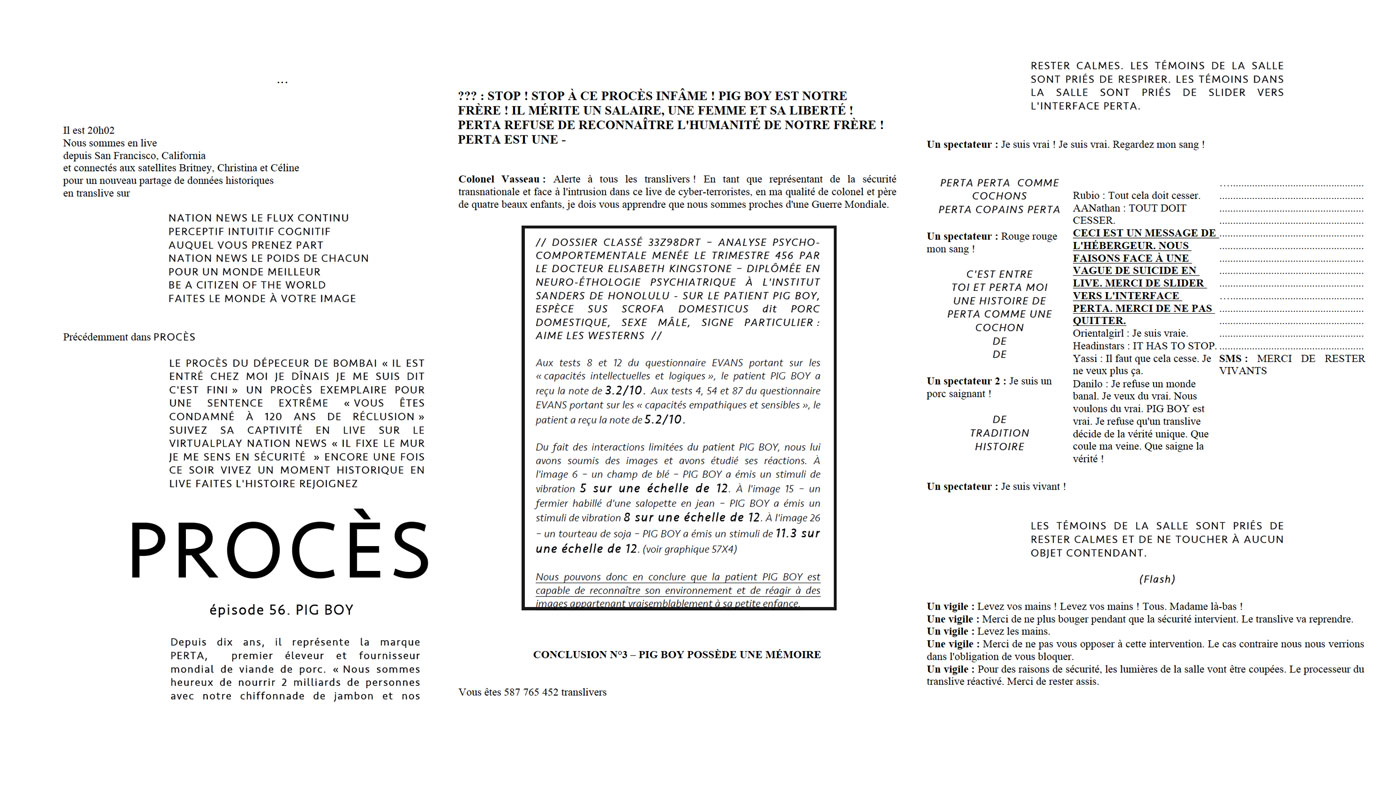
\includegraphics[width=17cm,height=9.555cm]{../assets/Pictures/100000000000057800000313E82B7C8B91FC9DF7.jpg}
\caption{Retranscription d'extraits de la deuxième partie de Pig Boy, pages 21, 31-32 et 37-38}\label{fig:fig-2--2-1}
\end{figure}

En concentrant cette deuxième partie de mon mémoire sur la deuxième partie du texte de Pig Boy, j'aimerais relever les éléments du texte qui permettent de reconnaître la forme de l'émission dès la lecture, et préciser en quoi ces éléments sont plus caractéristiques des nouvelles plateformes de diffusion sur internet que de la télévision et la radio (parties A et D). J'énoncerai également des considérations sur les \emph{topoi} récurrents d'Internet qui peuvent être trouvés dans les trois parties de la pièce (parties B et C). Enfin, je préciserai le parallèle que l'on peut faire entre la notion de spectacle au théâtre et dans le monde numérique (partie E). Toutes mes remarques s'appuieront également sur une analyse des enjeux de pouvoir présents sur Internet et notamment dans les politiques de plateformes actuels qui informeront la dimension supposément dystopique de ce texte.

\subsection{Interactivités, sources multiples}\label{interactivituxe9s-sources-multiples}

Qu'il s'agisse des résultats des pourcentages ou de la colonne «~Vos commentaires~», la deuxième partie du texte de Gwendoline Soublin est un texte à trous. Alors que l'histoire dont tu es le héros de la première partie ne semble pas pouvoir changer de voie, la deuxième partie implique les téléspectateurices et viewers de l'émission ainsi que les spectateurices de la pièce. Je définirai dans cette partie la notion d'interactivité, et sa filiation avec la communication internet.

\subsubsection{Un média interactif}\label{un-muxe9dia-interactif}

On définit comme interactive une interface qui présente plusieurs natures de médias (son, vidéo, texte\ldots) et qui réagit aux actions des utilisateurices. C'est le cas aujourd'hui d'à peu près n'importe quelle page internet. Menus déroulants, incrustations d'images animées, ou simplement hyperliens renvoyant à d'autres parties du site. Les forums de discussion, en plus d'être des supports interactifs, permettent non seulement d'interagir avec la machine mais aussi avec d'autres utilisateurices. Au contraire, la littérature n'est pas réputée pour être un média interactif, sauf peut-être aux quelques exceptions de la littérature hypertextuelle, des histoires dont le·la lecteurice est le héros ou de la poésie combinatoire de Raymond Quenaud{[}@raymondqueneauCentMilleMilliards1961{]}. Nous pourrions même dire qu'il s'agit plutôt des modalités de réception de l'œuvre que d'interaction, le matériau ne se modifiant pas à proprement parler mais étant seulement lu différemment. L'enjeu du \emph{translive} de la deuxième partie est d'impliquer les \emph{translivers} dans le déroulement du show, pour les amener à en consommer le contenu. Cependant, en laissant certaines parties du texte vides, Gwendoline Soublin laisse aussi la possibilité aux mises en scène de faire participer les spectateurices de la pièce, aux même titre que les autres \emph{translivers}, faisant ainsi du public de la salle des voyeureuses ayant une existence narrative au sein de l'histoire.{[}@vegaTransmediaGrandeConvergence2012a{]} Notons qu'il ne s'agit pas d'une œuvre transmédia telle que la définit Henry Jenkins~: bien qu'elle soit interactive , elle n'est pas immersive (la qualité d'un monde qu'on peut explorer de façon indépendante à l'histoire, comme dans les jeux vidéos) ni participative (les mondes qui sont construits en partie par les utilisateurices, par l'intermédiaire des \emph{fan fictions} par exemple).{[}@noussommesiciNoShowShowmustgoonTout{]}

Cet enjeu est traité différemment selon les œuvres du corpus. La création radiophonique fait exister les \emph{translivers} et les téléspectateurices comme deux entités différentes qui ont leurs présences sonores respectives dans la pièce mais se débarrasse complètement de l'aspect participatif du texte. En effet, sa mise en place nécessiterait une interface différente, par exemple une émission plateau en direct ou un site d'écoute à la demande qui pourrait prendre en charge l'influx des auditeurices. Telle quelle, la forme de la création radiophonique réalisée en amont et diffusée en amont ne permet pas l'interaction du public. Les mises en scène du Théâtres de l'Entre-Deux et du Bruit des Cloches prennent toutes les deux le parti de considérer le public de la salle et les téléspectateurices de la pièce comme une même entité. Les spectateurices sont donc complètement inclus·es, au même titre que les autres viewers dans le processus de vote de l'émission. Le vote s'effectue à main levée pour Théâtres de l'Entre-Deux et selon un système humoristique d'onomatopées pour le Bruit des Cloches («~Pour voter oui, répondez *bruit de cochon*, pour voter non, répondez *deux bruits de cochon*, pour voter ne se prononce pas, répondez *trois bruits de cochon*~») qui transforme la salle en porcherie l'espace de quelques secondes. Ces deux systèmes n'étant pas très précis, ils permettent d'annoncer les conclusions (qui sont, elles, écrites dans le texte) sans que celles-ci ne semblent trop hors de propos. Les pourcentages sont coupés dans les deux mises en scène, et Théâtres de l'Entre-Deux invente même «~avec le vote des translivers~» avant d'annoncer les résultats, ce qui ajoute une donnée inconnue aux spectateurices et permet de brouiller les éventuelles tendances qui serait identifiables dans la salle (une unanimité par exemple). Enfin, la mise en scène de Détour 21 supprime tout simplement la participation du public de la salle et la présence même de téléspectateurices dans la pièce~: le translive n'est pensé qu'en distanciel, et les spectateurices sont des translivers. Dans la version présente, les pourcentages ne sont pas indiqués et la participation des translivers aux votes n'est même pas avérée, ce qui permet d'accentuer l'inéluctabilité de la sentence et le procédé de manipulation dans l'émission qui fait croire à une agentivité des viewers. Cependant, nous aimerions à terme mettre en place un système de vote réel, dans l'idée que l'incongruité des conclusions et la méfiance vis-à-vis des autres spectateurices se fera d'autant plus forte si les participant·es votent vraiment~: le système totalitaire et biaisé dans lequel Détour 21 inscrit la deuxième partie n'en sera que plus tangible. La création radiophonique décide aussi de faire ressortir cet aspect en annonçant des pourcentages de plus en plus incohérents (lors du vote final~: «~oui 53~\%, non 48,6~\% , s'en remettent aux translivers 92~\%~»).

L'idée de réellement faire voter les spectateurices d'une pièce de théâtre a déjà été expérimentée auparavant. Par exemple, le spectacle \emph{Le NoShow} créé en 2013{[}@noussommesiciNoShowShowmustgoonTout{]} proposait un vote réel par un système de numéro court sur lequel le public de la salle envoyait un SMS de choix, qui était ensuite utilisé dans la pièce. Cependant, ce système nécessite un support technique supplémentaire, qui n'est pas à la portée de toutes les compagnies, ni de tous les théâtres (il faut une infrastructure dans laquelle le réseau peut être maintenu). Dans \emph{Pig Boy}, les SMS vont dans les deux sens, car certains sont aussi supposés être envoyés sur les téléphones des utilisateurices. Ce deuxième cas est plus problématique car il nécessite un accord préalable des spectateurices pour l'utilisation de leur numéro, et même une collecte, les théâtres n'ayant que rarement des listes de contact de leurs spectateurices qu'ils ont le droit d'utiliser. En effet, dans chacune des mises en scène, les SMS du texte sont soient dit par les voix de l'interface du translive, soit projetés sur l'écran dans le cas de Détour 21.

Les quatre instances du translive dans lesquelles l'espace des commentaires est ouvert s'organisent en trois colonnes dans le texte~: la colonne de gauche, qui donne le discours dominant de la plateforme (Présidente Shanon, Maître Spare ou Katsue Matumato), la colonne du centre qui indique les commentaires des translivers, et qui sont toujours investis par les mises en scène et la mise en onde selon divers procédés (décrits dans l'annexe 1~: Répartition des voix), enfin la colonne de droite, intitulée «~Vos commentaires~» lors de sa première occurrence, et qui reste systématiquement vide. Cette section, qui rappelle les messages par défaut «~Envoyez un message~» ou «~Commenter en tant que {[}nom de l'utlilisateurice{]}~» dans les interfaces de \emph{chat},indique une participation potentielle du·de la lecteurice et par extension des spectateurices de la pièce. Cet élément n'a à ce jour été investi par aucune des mises en scène existantes, essentiellement pour des raisons techniques~: difficulté de mise en place, de transportabilité selon les théâtres\ldots{} Clara Ménard, metteuse en scène du collectif Détour 21, a proposé à son équipe de comédien·nes d'écrire eux·elles-mêmes des commentaires, mais ils n'ont finalement pas été gardés pour la version actuelle de la mise en scène. Il me semble cependant que cette colonne, aussi vide de texte soit elle, est en fait déterminante dans l'enjeu de l'interactivité et mérite qu'on lui accorde la plus grande attention. Elle nécessite effectivement une mise en réseau à un moment donné~: cela peut-être une retransmission en direct du spectacle à un public à distance qui pourrait réagir (on pense au procédé de \emph{\_jeanne\_dark\_} qui a ouvert la voix en 2020{[}@marionsiefert\_jeanne\_dark\_2020{]}) ou bien un système de serveur local auquel les spectateurices pourraient se connecter. Ce deuxième cas, qui restreindrait la participation aux personnes présentes dans la salle, nécessiterait de repenser complètement le statut du public de la salle, pas tant pour sa participation active à la pièce, qui est souvent expérimentée au théâtre, mais pour sa participation virtuelle alors même qu'il se trouve dans la pièce avec les comédien·nes. En effet, le type de discours qui est permis par l'anonymat et la distance dans les commentaires n'est probablement pas celui que se permettraient des spectateurices ayant ne serait-ce qu'un contact visuel avec les personnages de la pièce. De la même manière, on pourrait imaginer une salle se transformant en assemblée, où le public pourrait énoncer à voix haute son avis, mais la probabilité que ce procédé prenne sans une médiation préliminaire importante est assez basse, à moins d'être avec des publics particuliers (on pense par exemple aux enfants\footnote{Un exemple récent au Théâtre Nicole Loraux de l'ENS~: \emph{Et maintenant nous allons faire une fête épouvantable}, spectacle jeune public qui proposait aux spectateurices de commenter les passages des comédien·nes en direct, ce que les enfants ont fait avec joie, alors que les adultes s'y risquaient beaucoup moins.}).

En ce qui concerne les parties écrites qui émanent normalement des téléspectateurices, par exemple la vague de suicides qui est censée contaminer les viewers en distanciel et en présentiel, seule la mise en scène de Théâtres de l'Entre-Deux prend le parti de faire jouer cette partie au public. En effet, dans cette mise en scène, les deux accusateurices, les personnes qui se suicident et l'activiste anti-spéciste sont joué·es par des membres du public. Les complices viennent deux heures avant le début spectacle pour prendre connaissance de leur rôle auprès du metteur en scène Philippe Mangenot, puis se répartissent dans la salle avec le reste des spectateurices, ce qui donne une impression de spontanéité de leurs parties losqu'ils·elles prennent la parole. Le Bruit des Cloches, qui considère aussi le public comme les téléspectateurices, distribue toutes ces parties aux deux comédiennes. Les accusateurices sont des translivers à distance, qui sont donc dans le dispositif lumineux décrit en première partie et la vague de suicides est interprétée par les deux actrices qui se déplacent dans les allées entre les sièges du public pour figurer plusieurs personnages se suicidant. Le passage de l'activiste est complètement remanié~: au moment du show de Youri, une des deux danseuses s'arrête, retire son masque et s'excuse auprès de ces collègues, disant ne plus pouvoir faire la comédie alors que Pig Boy est en danger (reprenant ainsi les mots de l'activiste). Cela interrompt la représentation de Youri, mais menace aussi la représentation de la pièce \emph{Pig Boy} elle-même, le public de la salle ne sachant pas précisément ce qui est de l'ordre du jeu. Lors de la représentation à laquelle j'ai assisté, une femme au premier rang s'est levée, prête à venir en aide à l'actrice. Le passage des vigiles est aussi un moment qui tend à affirmer la fusion des téléspectateurices et des spectateurices de la pièce pour ces deux mises en scène (Détour 21 et la création radiophonique ont coupé ce passage). Le processeur du translive s'arrête momentanément, dans une tentative ultime d'arrêter le phénomène qui se propage grâce à l'interface, et pendant un temps le public se retrouvent face au \emph{off}, le plateau du translive sans ses personnages et son spectacle. L'espace de \emph{PROCÈS} se brise dans le texte, il est difficile de savoir si les répliques des vigiles sont adressées aux téléspectateurices ou au public, car la mise en forme est la même que dans l'émission, mais c'est aussi la mise en forme habituelle des textes de théâtre~: on pourrait donc croire que l'émission coupée, les personnages reprennent leur audience par défaut, le public. Lors de l'appel des différentes personnes dans la salle, les deux mises en scène appellent à la fois des noms de personnages présents dans la pièce (Tao Wong, le colonel Vasseau) ce qui tend à garder la temporalité de la pièce, et les noms de leur équipe technique (les régisseureuses, les metteureuses en scène\ldots) ce qui tendrait plutôt à briser l'illusion de la pièce et ancrer l'intervention des vigiles dans le réel. Ce double jeu permet de garder la frontière floue entre ce qui tient du spectacle et ce qui tient de la réalité, à l'échelle des spectateurices -- y a-t-il un problème de courant dans la salle ou est-ce écrit par Gwendoline Soublin~? -- et des téléspectateurices -- y a-t-il un problème de courant dans le translive ou l'intervention des vigiles fait-elle partie du show~?

Un dernier élément qui indique une participation des spectateurices organisée par le texte est la présence d'un triple scénario à la suite du vote final (p.51). Contrairement aux conclusions, ce dernier choix dépend du résultat du vote, même si l'issue des trois scénarios est en fait la même~: Pig Boy est mis à mort. Aucune des œuvres du corpus ne faisant réellement voter le public avec un système qui permettrait d'établir un résultat précis, chacune décide à l'avance du choix qu'elle fera. La création radiophonique et la mise en scène de Théâtres de l'Entre-Deux décident toutes les deux de couper les scénarios, passant du résultat -- «~coupable~!~» -- à l'annonce de la sentence par la Présidente Shanon. La mise en scène du Bruit des Cloches choisit le premier scénario, dans lequel le résultat penche pour OUI (88\%), et les comédiennes disent le texte rythmiquement, à la manière d'un rap. Cette diction accentue l'aspect de divertissement que prend cette mise à mort, et que nous étudierons plus précisément en fin de partie. Enfin, la mise en scène de Détour 21 choisit le deuxième scénario, celui dans lequel les votant·es décident de sauver Pig Boy et de le considérer innocent. Ce scénario est le plus invraisemblable, il raconte comment le porc se met enfin à parler, pour avouer sa culpabilité et demander sa propre mise à mort. Il correspond cependant parfaitement à l'intention dramaturgique de la metteuse en scène, qui veut souligner que l'émission est truquée et scénarisée du début à la fin, et que la sentence capitale est prévu à l'avance. Par ailleurs, puisque c'est la seule version où la parole n'est jamais laissée au porc, les spectateurices n'ont pas la preuve qu'il ne parle pas. Raconter sa logorrhée fantastique au discours indirect continue de tracer la ligne dramaturgique d'une parole maîtrisée et «~médiatisée~», dans le sens où elle n'est plus portée par le personnage concerné mais par l'infrastructure qui l'entoure et l'empêche.

La dimension d'interaction avec le public rappelle les émissions concours de télévision, comme \emph{The Voice}, où le vote du public est demandé et modifie l'issue de l'émission, son·sa gagnant·e. Il est important de rappeler que ce procédé, plus qu'une intention démocratique de libre participation, sert surtout à générer un profit considérable pour les chaînes de télévision, l'envoi du message de vote étant payant. On peut également faire le parallèle entre ce procédé et je jeu dont tu es le héros de la première partie~: ici, il s'agit d'un jeu à plus grande échelle, où l'agentivité présente n'est pas celle du personnages concerné. Tous·tes les participant·es s'expriment en lieu et place de Pig Boy pour décider de son sort.

\subsubsection{Codes formels~: multiplicité des sources et discours types}\label{codes-formels-multiplicituxe9-des-sources-et-discours-types}

Une autre particularité des flux internet est son essence multimédia. La plupart des pages web sont interactives, comme expliqué dans le début de cette partie, et rassemblent des contenus et des sources différentes comme du texte, des images, de la vidéo\ldots{} Dans la deuxième partie de Pig Boy, les différences de police permettent très vite au·à la lecteurice d'identifier des sources différentes, alors même que tout est techniquement textuel. Les didascalies indiquent parfois un média particulier, par exemple la musique d'\emph{Il était une fois dans l'Ouest} ou encore les SMS, qu'on imagine être envoyés directement aux translivers avec une notification personnelle. Le texte de la plateforme comme les jingles, indiqué en petites capitales, est aussi différencié des paroles des personnages~: on peut ainsi les imaginer sur deux médiums différents. Le texte de Gwendoline Soublin ressemble indéniablement, dans sa mise en forme, aux modes de communication issus du réseau internet, et plus spécifiquement des plateformes de \emph{stream} vidéo sur certains aspects. Je prends la plateforme \emph{Twitch }pour exemple, de manière à pouvoir tirer des parallèles avec la présentation formelle du texte.

La plateforme Twitch, lancée en 2011 et rachetée par Amazon en 2014, est à l'origine un service de \emph{streaming} dédié aux jeux vidéos. En effet, elle est en fait le résultat de la scission de la catégorie \emph{gaming} de Justin.tv, qui fonctionnait plus que les autres catégories. Elle propose à la fois du streaming en direct et des vidéos à la demande. La majorité du contenu repose donc sur le modèle du \emph{stream }personnel, où un joueur se montre en train de jouer, permettant ainsi la discussion, l'apprentissage du jeu par d'autres ou encore les tournois d'\emph{e-sport}. On peut décrire une fenêtre de stream type de la manière suivante~:

\begin{itemize}
\tightlist
\item
  En grand se trouve l'écran du joueur, sur lequel on peut voir le jeu auquel il est en train de jouer. Du jeu dépendent la plupart des paramètres que l'on voit, les points de vie, la temporalité du jeu, la boîte à outils, etc.
\item
  Très souvent, une petite fenêtre montre le \emph{streamer} lui-même, qui réagit à sa propre partie et au commentaires des viewers. Cette fenêtre est le plus souvent en bas, à droite ou à gauche, et peut être une image du streamer dans l'endroit où il se trouve (à la manière d'un \emph{videocall}) ou une découpe sur fond vert qui est incrustée directement dans l'écran de jeu.
\item
  Le \emph{chat} peut lui-même apparaître sur l'écran, selon l'envie du streamer, et certains messages peuvent être lus par une voix synthétique. La fenêtre est aussi disponible aux viewers dans l'interface de Twitch sur la droite, elle est peut être visible ou non.
\item
  Les conditions d'accès au \emph{chat} peuvent varier, allant de n'importe quelle personne avec un compte Twitch à l'exclusivité pour les followers, mais de manière générale ils sont ouverts aux comptes dits «~vérifiés~», c'est à dire dont la validité a été confirmée par un numéro de téléphone attribué. La plupart du temps, un message de bienvenue stipule les règles du \emph{chat} avant que l'on puisse y participer, des prescriptions de bienséance essentiellement (ce qui fait penser au SMS d'introduction du translive dans la pièce).
\item
  La plupart des messages concernent le stream en cours~: réactions, aide au joueur\ldots{} Les utilisateurices ont également tendance à se répondre les uns les autres quand des questions sont posées ou simplement pour réagir ensemble. Un système de \emph{tag} permet d'identifier le message précédent auquel un message envoyé répond.
\item
  On trouve aussi régulièrement un bandeau, en haut ou en bas, qui indique le plus souvent le pseudo de la dernière personne ayant souscrit à la chaîne (abonnement payant) et la dernière personne l'ayant suivie.
\item
  Les sons présents sont ceux du jeu, la voix du streamer et parfois la voix synthétique des commentaires, et certains sons liés à l'activité des viewers, comme le signal d'un renouvellement d'abonnement (qui est souvent caractérisé par un bruit d'argent cliquant ou de machine de banque)
\end{itemize}

\begin{figure}
\centering
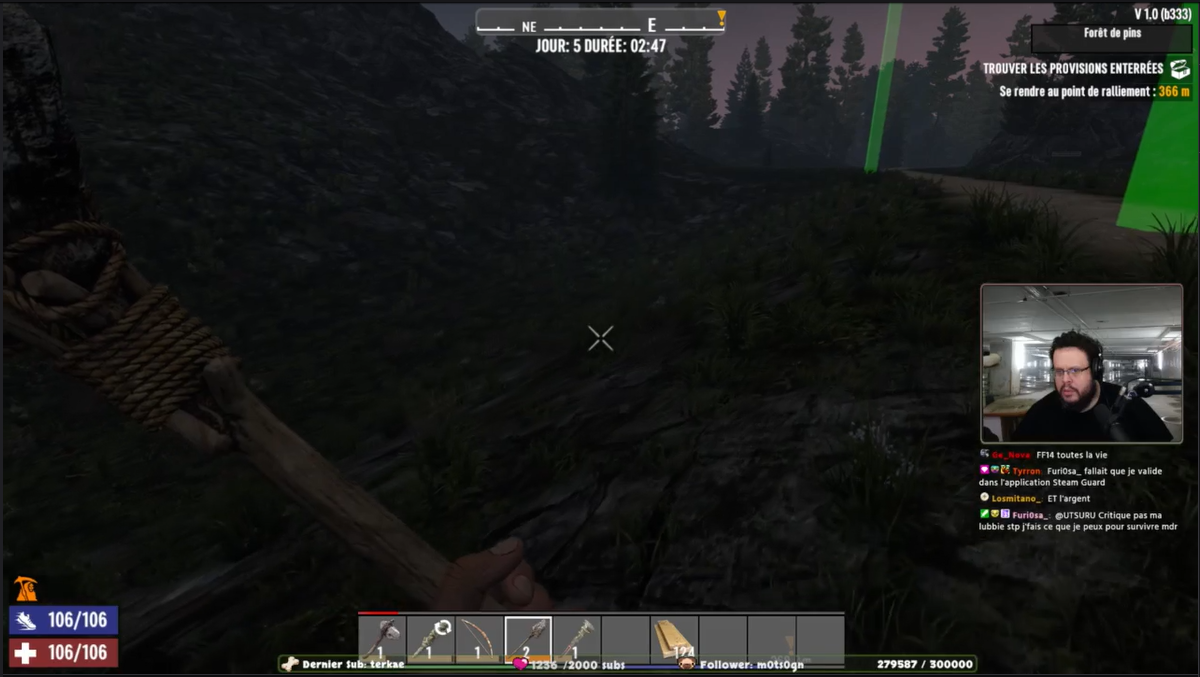
\includegraphics[width=17cm,height=9.59cm]{../assets/Pictures/10000201000004B0000002A59C804766341ECEC8.png}
\caption{Mynthos, 279 600 followers, sur 7 Days to Die.}\label{fig:fig-2--2-2}
\end{figure}

\begin{figure}
\centering
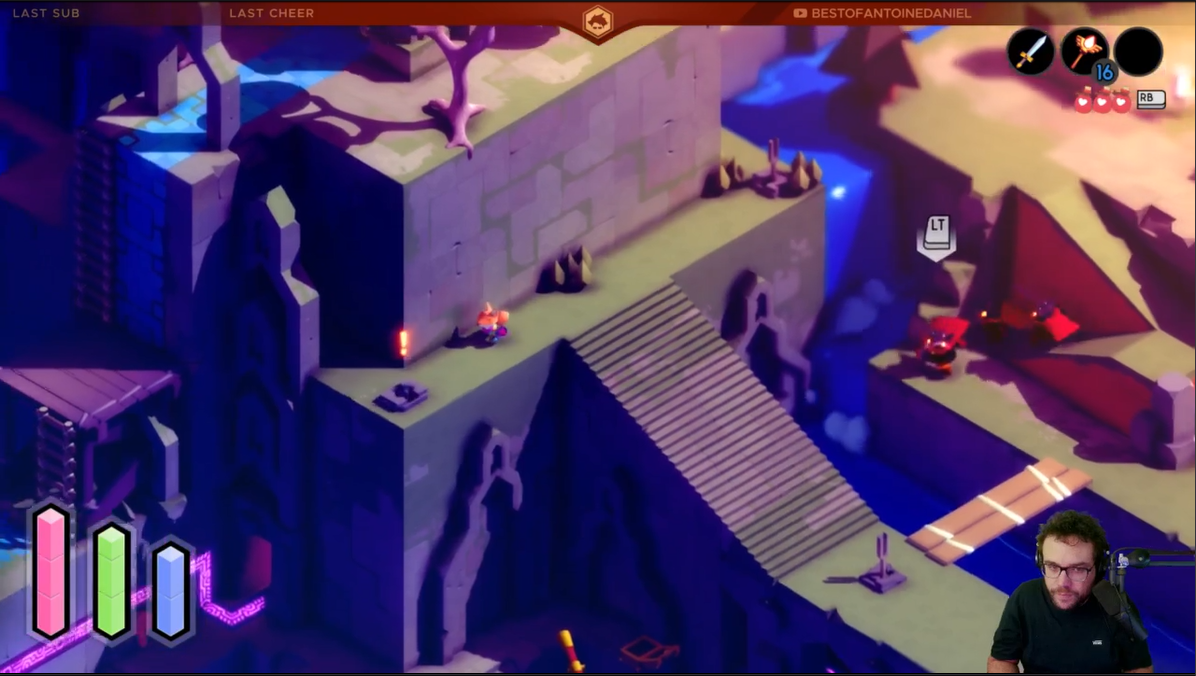
\includegraphics[width=17cm,height=9.608cm]{../assets/Pictures/10000201000004AC000002A4296D0393AE6C478A.png}
\caption{Antoine Daniel, 1 million de followers, sur Tunic.}\label{fig:fig-2--2-3}
\end{figure}

Néanmoins, les créateurices de Twitch ont aussi progressivement proposé d'autres contenus, comme des discussions, d'abord liées aux jeux vidéos, puis d'autres contenus créatifs (rassemblés sous l'étiquette \emph{creative} par Twitch) et enfin des contenus divers (catégorie \emph{IRL}) et notamment journalistiques, comme des lectures de textes scientifiques ou des matinales d'information. Cette dernière catégorie est investie majoritairement par des streamers situés à gauche de l'échiquier politique{[}@LecturesFeministesStream{]}, qui vulgarisent les écrits théoriques et commentent l'actualité. J'aimerais prendre le cas de la chaîne d'Ostpolitik, qui propose des revues de presse, et dont le contenu journalistique peut donc s'apparenter aux médias d'information plus traditionnels comme les journaux télévisés. J'ai basé mon analyse sur un stream du 26 juillet 2024 ayant lieu de 12h à 14h. En plus des caractéristiques communes avec les streams de gaming, voici les éléments saillants que j'ai pu relever dans ses streams et qui trouvent écho dans le texte de Gwendoline Soublin.

\begin{itemize}
\item
  Le \emph{chat} contient des formules idiomatiques de salutations en début et en fin de stream~: pour Ostpolitik, on retrouve par exemple divers variations de «~bonjour la gauche~», ou des formules plus générale comme «~salut à tous~» qu'on peut apparenter aux «~Hey~! Salut salut.~» de début de translive.
\item
  Pendant la durée du stream, le \emph{chat} comprend essentiellement des réactions à l'actualité et aux propos du streamer (comme «~la honte~» ou «~GG~» -- \emph{good game} à la base, qui marque plus généralement l'acquiescement ou «~bravo~»), des blagues et des questions (dans ce cas-ci, pertinentes, mais qui peuvent devenir hors sujet lors de streams plus gros, ou la modération est plus fastidieuse et procède donc par priorité). Dans cet exemple qui se situe pendant les jeux olympiques 2024, on trouve également des opinions qui ont attrait à des faits plus généraux, par exemple «~BOYCOTT JO~», qui peuvent faire penser aux slogans de certains translivers comme «~FREE PIG BOY~».
\item
  L'utilisation des sondages est assez répandue, et l'avis de l'ensemble des viewers peut être demandé simplement, notamment quand des réponses commencent à s'esquisser dans le \emph{chat}, de manière à établir des pourcentages.
\item
  La présence de jingles (composés par le·a streamer ou non) ainsi que d'éléments audiovisuels référencés (textes ou images accompagné·es de sons) ponctuant le déroulement du stream ou les actions des viewers est aussi très courante, ce que le stream a en commun avec les émissions des médias télévisuels et radiophoniques. Il y a également dans ce stream spécifique un bandeau déroulant qui indique le programme de la matinale, comme sur certaines chaînes télévisuelles, d'information en continu notamment. Ces deux éléments ajoutent à la multiplicité des sources présentes, et se retrouvent dans le texte de \emph{Pig Boy 1986-2358} par les différents encarts qui ponctuent la continuité du procès.
\end{itemize}

On peut aussi noter quelques dissemblances avec le translive du texte~:

\begin{itemize}
\tightlist
\item
  Même si il y a une certaine autonomie de la discussion dans le \emph{chat}, le **streamer le lit et réagit aux blagues, précise certaines choses, alors que les commentaires du translive sont complètement indépendants des prises de parole des acteurices du procès dans \emph{Pig Boy 1986-2358}.
\item
  Le·a modérateurice n'est pas un algorithme mais une personne habituée au streamer et à ses limites. Elle se trouve directement dans le \emph{chat }avec les autres utilisateurices mais peut décider de supprimer des commentaires par exemple. Le·a streamer lui·elle-même modère aussi parfois, et il·elle peut utiliser des \emph{bots}\footnote{Petits algorithmes simples qu'il est nécessaire de programmer soi-même.} pour l'aider, mais il y a toujours une réflexion humaine derrière. Parfois Twitch régule aussi les flux, avec par exemple des fonctions de ralentissement comme le «~mode lent~» qui limite la fréquence des commentaires des viewers (un message toutes les 3~secondes, un message toutes les 30 secondes\ldots).
\end{itemize}

Les plateformes de streaming sont un médium qui est associé à un public jeune dans l'imaginaire commun, même si une partie importante des créateurices de contenu se situe plutôt dans la trentaine. Les communautés internet marquant également un certain désintérêt pour les contenus politiques, elles ont été un public cible à la fois pour les hommes et femmes politiques, ainsi que pour d'autres groupes idéologiques non représentés dans le débat public, qui se sont appliqués à proposer du contenu politique sous d'autres formes, et notamment par les opinions des inflenceureuses. On pense par exemple au stream \emph{\#SansFiltre} qu'a proposé Gabriel Attal, alors porte-parole du gouvernement, lors de la pandémie du COVID-19. L'idée principale de cette stratégie et de remplacer l'espace du meeting politique par une situation plus informelle (par des éléments comme la conversation libre et le tutoiement), et de faire passer des messages politiques de manière indirecte. Ce qui rend cette situation si différente d'un plateau télé ou d'une conférence de presse, ce n'est pas tant le caractère informel de la situation que son absence de journalistes, qui sont normalement les médiateurices qui font le lien entre la production de contenu informatif ou politique et nous. L'information, sans médiateurices et sans spécialistes, devient alors un terrain d'opinions. Cette guerre des opinions est très présente dans la deuxième partie de \emph{Pig Boy 1986-2358}, où le procès se déroule sans médiateurices et sans que l'auditoire ne soit présenté dans ses réactions comme un public averti qui sait comment se déroule un procès et peut s'y repérer sans médiation. L'espace du direct, bien qu'il soit composé de paroles médiatisées technologiquement, engage une «~démédiatisation~» de la parole, c'est-à-dire que les intermédiaires disparaissent.{[}@douyereYoutubeEspaceExpression2019{]}

Nous avons vu plus haut que certains streams Twitch avaient des points communs avec les flux télévisuels comme les jingles qui ponctuent le déroulement de l'émission ou encore des aspects formels comme les bandeaux déroulants qui ajoutent une strate d'information décorrélée de ce qui est discuté par les journalistes. Le média Blast va même jusqu'à demander si ces streams, «~c'est pas toujours de la télévision~»: il y a un plateau, des gens qui parlent de sujets d'actualité, des animateurices, des chroniqueurices, des invité·es. On peut trouver des streams appelés \emph{reacts}, où les streamers regardent des documents télévisuels et les commentent. De *même sur des réseaux sociaux comme X (ex-Twitter) ou Facebook, les publications reprennent essentiellement des extraits d'émissions télévisées. On remarque également une certaine perméabilité de la télévision et des plateformes de streaming, avec par exemple l'arrivée du streamer Hugo Décrypte sur la chaîne de télévision publique France 2 ou encore le présentateur Samuel Étienne qui est désormais streamer également.{[}@blastlesouffledelinfoTELEVISIONQUANDBOURDIEU2024, 3:22{]} Cependant, deux traits essentiels opposent la télévision (et la radio avec elle) aux logiques des plateformes. Tout d'abord, les chaînes de télévision et de radio continuent de tenir une ligne éditoriale et de produire leurs émissions, là où la charge de production et de rentabilité incombe aux seul·es créateurices sur les plateformes de streaming. D'autre part, les flux télévisuels et radiophoniques descendent a priori uniquement de manière verticale, des chaînes vers les téléspectateurices/auditeurices, tandis que les plateformes organisent des flux à double sens, où le contenu arrive aux viewers et où les données de ces derniers remontent à la plateforme. Les consommateurices du contenu s'en font donc aussi les producteurices.{[}@dujarierTravailConsommateur2014, pp.5-18{]}

La dystopie du translive que nous présente Gwendoline Soublin dans \emph{Pig Boy 1986-2358} emprunte à chacun des deux médias. Le programme \emph{PROCÈS} semble être diffusé par une chaîne, \emph{Nation News}, qui se présente comme un «~flux continu~», et «~auquel {[}les viewers prennent{]} part~» (p.21), et la présence du \emph{chat }et des informations en direct sur le nombre de participant·es tend à caractériser le direct qui provient des plateformes. Cependant le titre de la chaîne, la présence d'une multitude d'invité·es, la place dans le texte d'une voix de présentateurice qui s'adresse aux viewers, tous ces éléments renvoient plutôt à l'imaginaire de la télévision. On imagine donc une sorte de chaîne en continu, diffusée depuis une plateforme de streaming et par internet, qui aurait assimilé les codes de la télévision. Un monde, probablement, dans lequel la télévision ne serait plus un médium à part entière mais confondu dans les flux internet. Ce parallèle rappelle d'ailleurs les origines de la télévision~: la technologie vidéo n'était d'abord que du direct, il était impossible d'inscrire le signal vidéo sur un support. Les écrans de télévision étaient filmés avec une caméra argentique pour avoir des enregistrements de ce qui était diffusé en direct. L'histoire de la télévision est très liée à la technologie vidéo, qui est aussi celle utilisée dans les flux internet, et donc à la notion de direct. Le texte de Gwendoline Soublin s'amuse encore une fois à fonder son ambiance dystopique sur des similitudes entre passé proche et futur proche.

Dans les mises en scène de Théâtres de l'Entre-Deux et du Bruit des Cloches, les metteureuses en scène ont décidé de représenter le translive de la deuxième partie sans recourir à l'audiovisuel. Dans les deux cas, les commentaires sont dits par les comédien·nes. Pour rappel de la première partie de ce mémoire sur le traitement des voix, Théâtres de l'Entre-Deux propose un dispositif avec une pancarte qui indique le pseudo du personnage et une déformation en direct de la voix. Le Bruit des Cloches utilise quant à lui la voix modifiée du musicien en direct pour annoncer les pseudos et deux sons courts qui encadrent la prise de parole de la comédienne qui fait les commentaires. La création radiophonique fait bien évidemment aussi dire les commentaires par des voix, assez réalistes, qui existent dans un espace différent de la prise de parole des acteurices du procès par le fond sonore qui les accompagnent. Ce sont comme des échantillons de vie, et on apprend beaucoup de la situation du viewer par l'environnement sonore qui apparaît lors de sa prise de parole. Seul le collectif Détour 21 propose de montrer le \emph{chat }par le médium duquel il est issu, en projetant le texte des commentaires sur un écran sur le côté de l'espace de jeu des comédien·nes, celleux-ci ne prenant en charge que les acteurices du procès et les épisodes pré-enregistrés. La prise de parole des personnages qui sont soumis au flux de commentaires retrouve donc l'intelligibilité des paroles de streamers, qui ne sont pas interrompues par le \emph{chat}. Lorsque le \emph{chat} lui-même est ponctué par des messages de l'hébergeur ou des virus, ceux-ci sont diffusés sur le grand écran de fond de scène. Les SMS sont affichés sur l'écran par l'intermédiaire d'un bandeau déroulant, ce qui rappelle les bandeaux que j'ai relevés sur Twitch ou les chaînes d'information en continu~: l'écran est lui-même une interface contenant de multiples sources.

\subsection{Jouer, choisir}\label{jouer-choisir}

Seule la deuxième partie de \emph{Pig Boy 1986-2358} implique matériellement les spectateurices et téléspectateurices, cependant les notions de jeu et de choix traversent la pièce dans son intégralité. Elles se manifestent sous différentes formes, et j'essaierai de dresser une liste exhaustive des occurrences dans cette partie.

\subsubsection{Jeux}\label{jeux}

Dans la première partie, plusieurs jeux s'entrelacent à plusieurs échelles. Tout d'abord, le procédé formel dans l'écriture des choix fait penser aux livres dont tu es le héros, un genre plutôt présent dans la littérature jeunesse. L'idée est qu'après une portion de l'histoire, le·la lecteurice puisse faire un choix parmi deux propositions, et que ce choix l'amène à un autre endroit du livre~: ainsi, le déroulé du récit dépend des choix qui sont faits par le·la lecteurice, même si toutes les parties sont écrites à l'avance. Dans \emph{Pig Boy 1986-2358} chaque paragraphe de narration, écrit à la deuxième personne du singulier, est suivi par un dilemme entre deux choix écrits en capitales, et ce jusqu'à la fin de l'histoire. On peut noter une occurrence d'un choix à trois entrées, une occurrence d'un choix unique et une occurrence d'un choix à sept entrées, toutes identiques. Il s'agit des trois derniers choix du texte, qui n'interrompent donc pas le procédé formel mais le dépassent en fin de partie. Bien que ces choix prennent la même forme que dans un livre dont tu es le héros, ici il n'y a aucune agentivité du·de la lecteurice (et donc des spectateurices) puisque le récit avance de façon linéaire dans tous les cas. Le sens du texte tend à impliquer que le personnage principal n'a pas non plus d'agentivité, nous verrons plus loin en quoi ce procédé soulève l'inéluctabilité de son destin. À partir du choix «~1 - VOUS REMERCIEZ LE COCHON POUR SA VIE 2 - VOUS RÉFLÉCHISSEZ AU PROGRAMME TÉLÉ DU SOIR~» (p.11), le corps du texte n'indique plus quel choix est fait par le personnage, ce qui renforce son manque d'agentivité, et inscrit le procédé formel dans une dynamique poétique répétitive plutôt que dans une nécessité de sens.

Dans la mise en scène de Théâtres de l'Entre-Deux, chaque choix annoncé est ponctué par des «~yes~» de satisfaction ou des «~iiich~» de défaite, comme si quelque chose de très important se jouait, ou qu'il s'agissait d'un match serré entre deux camps (peut-être les deux camps qu'illustrent la création radiophonique avec ses deux voix). C'est un jeu, mais un jeu qui est pris très au sérieux, qui tient à cœur les comédien·nes et qui, en début de partie du moins, peut vraiment tourner d'une manière ou d'une autre. Rien n'est encore écrit. Ce jeu est cependant comme regardé depuis l'extérieur~: le personnage principal est passif et ne fait pas de commentaires sur ce qu'il lui arrive. Dans la mise en scène du Bruit des Cloches, le jeu des comédiennes ne fait pas vraiment ressortir la dimension ludique de l'histoire dont tu es le héros~: par leur ton, on comprend dès le commencement qu'il n'y aura pas de choix possible.

Le jeu télévisé Miss France prend aussi une part importance dans le texte de la première partie~: c'est la seule émission que la famille Bouquet s'autorise à regarder, et le choix final entre les deux miss régionales ponctue régulièrement les choix du texte, illustrant les années qui passent puisque ce jeu est un programme annuel. L'émission est aussi un indicateur de classe sociale dans l'imaginaire commun, et place la famille du personnage dans un certain cadre, notamment en ce qui concerne les masculinités et les féminités canoniques de leur milieu. Le choix à trois entrées, page 18, renvoie également à un jeu télévisé, \emph{Qui veut gagner des millions~}: «~1 - VOUS DEMANDEZ LE VOTE DU PUBLIC 2 - VOUS PRENEZ LE 50/50 3 - VOUS APPELEZ UN AMI~». Ce choix, qui renvoie à une échappatoire lorsqu'on est bloqué dans ce jeu, pose ici paradoxalement l'impossibilité du personnage d'échapper aux huissiers, et donc à son destin, et introduit la scène du suicide final (p.19). Enfin dans la deuxième partie de \emph{Pig Boy 1986-2358}, l'émission \emph{PROCÈS}, que j'ai étudié sous l'angle de l'interactivité dans la partie précédente, correspond également aux codes formels du jeu télévisé.

\subsubsection{Paradoxe du choix}\label{paradoxe-du-choix}

Tous ces jeux demandent à un moment de leur déroulé le choix des participant·es. Hors dans la pièce, et notamment dans la première partie, le paradoxe de tous ces choix énoncés face à l'absence de choix pour le personnage est frappant. Théodore Bouquet, petit éleveur de porcs breton qui reprend une exploitation endettée en 2014, n'a pas le choix. Bien que la pièce soit fictive, le récit du personnage principal s'inspire très précisément de notre réalité.

En 2014, cela fait plusieurs années que le coût de production des porcs augmente (notamment le coût de leur alimentation), et donc que le prix du porc, déterminé à l'échelle nationale par le Marché du Porc Breton, augmente aussi. Les grands industriels achètent la viande de porc moins chère à d'autres pays européens, ce qui provoque une crise de l'offre~: trop de porcs sont produits, et ne sont pas vendus, ou à perte. Les prix n'augmentent pas pour les consommateurices en fin de chaîne (les acheteureuses en supermarché), c'est donc un gain sur la productivité qui doit venir des exploitant·es pour «~redresser la barre~» (expression utilisée par le personnage de la première partie page 17). Les grandes exploitations ne réduisent pas le coût de production, contrairement à ce que l'on pourrait croire, les marges sont en fait prises sur les cotisations sociales (la protection sociale des salarié·es) et sur une «~simplification administrative~» (des mesures de relâchement des contrôles sanitaires et de relèvement des seuils maximum de porcs qui permettent les exploitations géantes). Il est aussi important de soulever que la surproduction est générée par les «~acheteurs de la grande distribution~» (expression également utilisée par le personnage principal, page12), qui ont intérêt à avoir trop pour choisir avec quoi faire leurs produits transformés~: la pression de ces acheteurs, ainsi que l'ouverture du marché à l'import-export, permettent de peser sur le prix du porc français. Le jeu de l'import-export n'est qu'un moyen parmi d'autres que se donnent les opérateurs pour faire baisser les prix des matières premières, l'objectif étant de pousser la production de viande à moindre coût, afin de fournir les conserveries et autres fabriques de plats cuisinés, avec la circonstance aggravante, par rapport aux productions végétales, de l'horreur de l'univers concentrationnaire et des souffrances imposés aux animaux et aux humain·es dans la production porcine.\footnote{Ces informations générales proviennent de diverses sources journalistiques et médiatiques sur le sujet, voir notamment {[}@gerardflorensonCrisePorcineSpecificite{]}.} Dans ces conditions, les petites exploitations subissent avec d'autant plus de violence la crise, et le destin de notre personnage Théodore Bouquet est malheureusement très commun. Lors d'une représentation de la première partie de la pièce par le collectif Détour 21, dans une ferme du Tarn, plusieurs paysan·nes ont d'ailleurs confirmé par leur témoignage la justesse du texte de Gwendoline Soublin. J'aimerais souligner ici un choix de mise en scène particulièrement pertinent. Théâtres de l'Entre-Deux décide d'illustrer l'anecdote du jeune exploitant, voisin du personnage principal, écrasé par un tracteur alors qu'il s'y était menotté par revendication de la manière suivante~: un comédien monte le podium qui est en milieu de scène, lentement, et continue de marcher jusqu'en haut, jusqu'à faire un pas dans le vide et donc tomber d'un bon mètre. Cette métaphore de la marche, du pas en avant coûte que coûte, peu importe le vide, traduit à mon sens l'inéluctabilité de sa mort, et son impossibilité d'y échapper, et résonne avec le destin du personnage principal.

Au-delà du procédé formel des choix ponctuant le texte, la notion de choix, et son absence, apparaissent également dans le corps des paragraphes de narration. Le personnage principal est fils unique, c'est donc le seul héritier de la ferme de son père~: «~tu restes le seul fils. Le seul espoir. Le seul choix.~» (p.10). Faire le choix de ne pas être exploitant agricole impliquerait de terminer la lignée professionnelle qui se perpétue dans sa famille, et on peut imaginer comment ce premier choix, bien qu'il existe, soit inenvisageable~: l'oxymore «~le seul choix~» permet de traduire cette nécessité. Son orientation professionnelle vers une filière courte est dans la continuité de ce premier choix, et sa vie semble suivre un cours qu'il a désiré jusqu'au point de bascule, qui advient lorsque le père se pend. Ce moment du texte est très structurant dans toutes les mises en scène et la mise en onde, et annonce la lente déchéance jusqu'à la fin de la partie. Le suicide du père, c'est le premier choix qu'il subit, qui fait de lui un \emph{pig boy} contre son gré. Cela tranche très sèchement avec le récit qu'il se fait de lui-même, et entame son agentivité, qui ne cessera pas de décroître par la suite. Progressivement, les choix essentialisent le dilemme, opposant une action au statut de \emph{cow-boy}, et menaçant donc l'intégrité du personnage et de son rêve si il opte pour le premier choix~: «~1~- VOUS PRENEZ QUELQUES JOURS DE REPOS 2~- VOUS ÊTES UN COW-BOY~» (p.15), «~1~- VOUS ACCEPTEZ LA LIQUIDATION DE VOTRE EXPLOITATION 2~- VOUS ÊTES UN COW-BOY~» (p.17). Garder le statut de cow-boy implique en fait aussi des actions, et c'est la volonté du personnage de «~ne rien lâcher~» qui va finir par l'emmener vers sa fin. Le «~non-choix~» d'acheter des santiags page 18, dont les deux entrées sont identiques -- VOUS ACHETEZ DES SANTIAGS -- et qui donc brise l'illusion de choix qui existait avant, est paradoxalement la première occurrence qui semble choisie, parce qu'elle répond à une envie de longue date, et fait donc franchement plaisir au personnage. Le choix du personnage de se faire plaisir, de commencer à vivre d'une certaine manière, signe son arrêt de mort. Son suicide spectaculaire, même s'il signe la fin de son histoire, marque aussi la reprise de son agentivité à la vie, contre un système qui le maîtrise et le broie depuis longtemps.

\subsubsection{Voies}\label{voies}

On pourrait cependant arguer que le personnage, malgré le peu de marge de manœuvre qu'il a, décide une partie de son parcours, et choisit une «~voie~», et une façon de vivre les évènements, à défaut de choisir ce qui advient. L'épisode de Mathilde est particulièrement parlant~: a priori, il s'agit simplement d'un chagrin d'amour, le désir d'une fille qui ne s'intéresse pas à lui, la petite tragédie des filles qui partent à la ville pour étudier et quitter leur campagne. Cependant, là où il pourrait avaler son humiliation et continuer son chemin, le refus de Mathilde marque le début de son isolement~: cette réaction s'inscrit dans la continuité d'une masculinité qui ne demande pas d'aide. Dans le long paragraphe entre les pages 14 et 15, on trouve plusieurs itérations de ce fonctionnement~: «~Si on t'accuse d'être un mauvais exploitant, tu ne perdras pas l'appétit.~», «~Tu ne prendras pas des antidépresseurs.~», «~Tu crées ta propre légende. {[}\ldots{]} Toujours seul.~». Le personnage s'accroche à lui-même, et refuse de se reposer sur quelqu'un d'autre. Refuse de prendre un ouvrier agricole pour l'aider, refuse de téléphoner à Solidarité Paysans. Lorsqu'il pense une première fois au suicide, une des choses qui l'arrêtent est la réalisation qu'il n'a personne à qui adresser son mot d'adieu. Le texte se transforme pour faire apparaître «~Tu te sens seul~» (p.15). La mise en scène de Théâtre de l'Entre-Deux, par l'imaginaire de la folie qu'il convoque et que j'ai développé en première partie de ce mémoire, accentue cette solitude, tout comme le fait le choix de répartition du texte de Détour 21, qui fait dire les passages renvoyant à sa solitude à l'unisson. Gwendoline Soublin dépeint aussi en creux ce que le personnage pense des manifestations d'agriculteurices~: «~Tu éteins la télé. Tu n'as pas de temps à perdre. Tu es un cow-boy~». Là encore, face à une révolte sociale de grande ampleur, le personnage décide de s'isoler, et de comprendre sa difficulté comme un manque de force de sa part plutôt que comme un problème systémique, auquel seule une mobilisation commune pourra remédier.

\subsection{Topoi de la solitude et de la mort}\label{topoi-de-la-solitude-et-de-la-mort}

\subsubsection{Omniprésence de la solitude}\label{omnipruxe9sence-de-la-solitude}

Cette sensation de solitude est très présente dans les trois parties du texte. Dans la première partie, les occurrences que je viens de relever suivent une trajectoire en trois temps~: le personnage enfant admire l'indépendance des cow-boys, puis il fait l'expérience du rejet et décide de faire de sa propre solitude une force, mais c'est cette solitude qui le ronge, devenant finalement une sensation insupportable qui le rend fou.

Dans la deuxième partie, on retrouve en creux cette thématique de la solitude dans le passage de retour au calme, qui parle d'unité. Le translive, complètement dépassé par la vague de suicides provoquée par une soudaine ruée vers le vrai, propose un «~intermède musical~» accompagné d'un discours de méditation qui vise à calmer les viewers (p.39). Ce passage se concentre sur la transmission de l'idée que tous les viewers sont connecté·es les un·es aux autres et forment une unité tournée vers la vie. On peut déduire que si la plateforme tente de calmer ses consommateurices avec le sentiment d'appartenir à un ensemble, c'est qu'elle évalue leur plus grande peur comme étant le sentiment de la solitude extrême, d'absence de liens avec leurs pairs. Le jeu dépend du maintien en vie des viewers. Les mises en scène de Théâtres de l'Entre-Deux et du Bruit des Cloches ainsi que la création radiophonique interprètent ce passage avec une voix très douce, toutes féminines, proches des voix d'instructions dans les CD de méditation. Seule la mise en scène de Détour 21 choisit de faire dire ce passage à la présentatrice, seulement éclairée de sa tablette dans le noir complet, de façon très crispée. On sent bien que le personnage tente d'être rassurant mais sa voix suraiguë trahit sa tension~: la présentatrice doit tenir le translive alors qu'elle est elle-même à bout. Son «~Fermez les yeux~» est d'abord une supplique, puis devient un ordre strict, à l'impératif.

Ce personnage de présentatrice, interprétée par Alisma Boulay du collectif Détour 21, est plus développé dans cette mise en scène que dans les autres, avec notamment l'ajout d'un passage seul au début et à la fin de la deuxième partie, hors translive, qui permet de mettre en exergue la solitude du personnage, et donc de le lire différemment pendant la partie. Le passage du début, qui dure plus de cinq minutes, montre le personnage d'Alisma se préparant, se maquillant et enfilant la perruque rose qu'elle arborera pendant le translive. Elle a l'air très triste et très seule, et lorsque le décompte du début du translive se met en route, elle se plaque un sourire immense sur la figure, qu'on peut légitimement interpréter comme faux tout le restant de la pièce (figure~\ref{fig:fig-2}). Ce personnage, avec son sourire forcé, a l'air au bord du craquage à tout instant.

\begin{figure}
\centering
\includegraphics[width=17cm,height=11.347cm]{../assets/Pictures/100000000000178000000FB057924CC19D0CB325.jpg}
\caption{Le personnage de la présentatrice, collectif Détour 21, deuxième partie. Photo d\textquotesingle Amandine Benoit.}\label{fig:fig-2--2-4}
\end{figure}

Dans la troisième partie, le personnage de la truie est complètement seul, même si il se sent traqué. La truie marche seule dans la forêt, pour accoucher de ses petits loin des humain·es. Elle décrit également voir d'autres animaux, mais ces descriptions d'animaux-chimères sont si irréelles qu'on ne sait pas où se situer~: sommes-nous sur une terre où les animaux sont tous hybrides ou cette truie est-elle en train d'halluciner, rongée par l'aliénation, seule dans son box de laboratoire~?

\subsubsection{Répétitivité}\label{ruxe9puxe9titivituxe9}

Il est intéressant de remarquer que les trois parties, bien qu'elles soient drastiquement différentes par leur époque, leur ambiance et leur style littéraire, finissent en fait de la même manière~: la mort du Pig Boy dans un feu. Chacun des personnages se dirige vers la mort. Le choix peut sembler plus évident dans la première partie, dans laquelle le personnage se suicide, et la dernière partie, dans laquelle la truie décide d'entrer dans une forêt incendiée, mais le choix de la mort est aussi présent dans la deuxième partie, puisque des personnages choisissent la mort de Pig Boy. Plus encore dans la mise en scène de Détour 21, où le deuxième scénario est présenté, Pig Boy choisit sa propre mise à mort. Pour la fin de la première partie, la mise en scène de Théâtres de l'Entre-Deux a fait le choix d'ajouter la phrase «~Et toi, tu brûles.~» après la fin écrite par l'autrice, afin de renforcer l'image de l'incendie.

Le sous-titre de la pièce, qui est très rarement présent dans les feuilles de salle ni même dans les informations qu'on peut glaner sur le paratexte ici et là, mérite aussi d'être mentionné~: \emph{replay du devenir homme}. On peut faire plusieurs hypothèses quant à la signification de ce sous-titre, dans tous les cas le mot «~replay~» tend à valider l'hypothèse d'un \emph{pattern} de répétition dans les trois parties. Quelle est alors la nature de ce «~devenir homme~»~? À mon sens, la pièce montre trois chemins \emph{vers }l'humanité, trois chemins différents, parallèles. Théodore Bouquet retrouve l'humanité dont il a été privé en reprenant le pouvoir sur sa propre vie, en récupérant son agentivité, même si celle-ci le conduit à la mort. Dans la deuxième partie, la plus sombre, l'ensemble des translivers accèdent à leur humanité par le consensus de la mise à mort, par leur cruauté en quelque sorte, et la sensation de faire un en tant qu'espèce, vis-à-vis de l'animalité. La troisième partie raconte le chemin d'une bête, de la même espèce que le condamné de la partie précédente, vers son libre arbitre et sa liberté matérielle. Elle meurt aussi dans cette quête, mais son récit et plein de joie et d'espoir. Le fait que les trois chemins amènent à la mort peut poser la question~: est-ce la mortalité, ou le rapport à la mortalité, qui fait de nous des humain·es~? Gwendoline Soublin n'y répond pas frontalement, et laisse coexister différentes interprétations.

Un des éléments qui m'a frappé quand j'ai vu les mises en scène par rapport à la lecture du texte, c'est justement les choix de représentation de la mort. Dans la version de Théâtres de l'Entre-Deux par exemple, les deux premières morts sont très spectaculaires. Leur place en fin de parties leur donne déjà un statut particulier, mais elles sont également appuyées par une représentation très dramatique, avec des papiers rouges symbolisant le feu, une chanson lancinante pour la deuxième partie et une longue pause sur l'acteur qui joue le Pig Boy qui meurt. Hors le paradoxe de ces morts est qu'elles sont complètement non-évènementielles. Le suicide d'un agriculteur, la mise à mort d'un porc noyé dans un principe d'émission récurrent, la perte d'un animal de laboratoire dans les alentours de bâtiments, ces trois scénarios n'ont a priori rien d'extraordinaire. Et le texte, qui développe l'histoire de ces personnages, propose évidemment une forme d'empathie pour eux mais garde à mon sens ce côté terre à terre, notamment dans la deuxième partie. La mort de la première partie, si on considère qu'elle est racontée à la première personne par l'exploitant lui-même, se doit d'être épique puisqu'elle imite les fins de westerns. Elle est souvent dit lentement par les comédien·nes, projetée fortement, comme une apothéose. Cependant, on perd la dichotomie du drame particulier, de la double échelle qui rend cette mort si difficile et si représentative de notre époque. Dans la deuxième partie, le texte original noie la mort de Pig Boy dans une multitude d'informations, une chanson d'adieu qui décrit la scène, le commentaire grotesque du personnage de présentateurice, de la publicité pour des casques dernière génération, pour la multinationale PERTA INFINITA et pour l'épisode suivant de l'émission. La mort ne fait pas évènement, ne secoue pas les tripes, on s'apitoie quelques temps et puis on passe à autre chose. La compagnie Le Bruit des Cloches décide de chanter le scénario ainsi que la chanson d'adieu \emph{Last Song for Piggy Boy} sur un tempo assez allant, ce qui dédramatise complètement la scène. Cela fait de cette mort un divertissement, une mascarade pour amuser le peuple. Au contraire, la mise en scène de Théâtres de l'Entre-Deux est beaucoup plus esthétique, les mouvements sont très beaux et très symboliques encore une fois~: par exemple, on passe une cravate au cou de Pig Boy à la manière d'un nœud de corde, elle porte donc ce double sens même en retombant en cravate. Dans toutes les mises en scène et la mise en ondes, la publicité pour gagner des casques DH15 a été coupée~: elle est pourtant très caractéristique de l'inscription de l'émission dans une logique de consommation. Ce petit détail est en fait très important pour rendre la mort très casuelle, sans importance. La mise en scène de la troisième partie par le Bruit des Cloches et elle aussi très épique~: la truie, qui s'extrait difficilement de son box, se relève dans un grand effort et se tient face à nous, presque humaine, alors que la forêt brûle et que la musique d'\emph{Il était une fois dans l'Ouest} retentit une dernière fois. Les choix de représentation des mises en scène privilégient donc plus souvent l'aspect dramatique des morts que leur aspect ordinaire.

Les trois personnages qui meurent sont très spectacularisés dans les mises en scène, avec l'imaginaire du cinéma, puis l'effervescence du jeu et la folie de l'illumination, et meurent simplement dans le texte. Et Miss Bretagne applaudit, et la plateforme dit merci, et l'incendie continue. Il me semble que là où le discours d'information est très capable de rendre habituelles des morts, de nous immuniser de l'empathie trop grande qu'il faudrait pour accuser le coup de tous les crimes et génocides de l'humanité, le théâtre en tant qu'art du drame a beaucoup de mal à faire passer des morts sur scène inaperçues. Le discours internet (quand il ne s'agit pas du discours d'information diffusé sur internet) présente généralement des images et des faits très bruts , et provoque donc un effet similaire à l'esthétisation théâtrale. Il s'agit là d'une similitude entre ces deux médiums, qui les opposent à la spécificité des médias d'information. La création radiophonique, à la frontière entre ces deux mondes, peut décider d'emprunter son discours à la voix d'information radiophonique, sans trop de difficultés, ou de privilégier une dramaturgie plus proche de celle du théâtre, qui fait drame. C'est aussi l'espace particulier du théâtre traditionnel, cette boîte noire, qui rend des faits mêmes les plus communs évènementiels. La création radiophonique, par sa proximité de médium avec la radio d'information, peut emprunter à l'un et l'autre des registres sans susciter la méfiance analytique de l'auditeurice.

\subsubsection{Nécropolitique}\label{nuxe9cropolitique}

J'ai exposé à la fin de la première partie de ce mémoire les procédés de voix synthétiques qui rapprochaient certains choix de mise en scène et de mise en onde avec l'\emph{analog horror}. Dans la même intention, Détour 21 propose un moment qu'on peut difficilement décrire autrement qu'avec le mot chaos, qui est introduit par l'expression «~\emph{Out of the System~}» qui est scandée page 17. Cette expression peut renvoyer à un imaginaire autonomiste ou anarco-primitiviste, à l'utopie d'une vie \emph{off-grid} (hors du circuit de l'énergie électrique) et hors du système, sous-entendu capitaliste puisque c'est le système dans lequel nous vivons, et dans lequel le personnage de la partie 1 vit également. On peut même penser à l'imaginaire survivaliste qui, dans le contexte états-unien, s'est réapproprié la figure du cow-boy. Pendant deux minutes trente, sur la chanson \emph{Our Love }d'Al Hazan et les Starr Sisters, dans une lumière rouge ponctuée de stroboscopes, les quatre interprètes se prêtent à quatre terribles tableaux~: l'une mêle désir et violence en dansant très sensuellement avec un grand couteau~; une autre s'enrobe intégralement le visage de film plastique jusqu'à l'étouffement~; les deux dernièr·es engloutissent une matière qui renvoie à de la viande, voire à des abats, un mélange de flageolets et de saucisses végétariennes. Ce passage illustre une forme de perte de contrôle qui se manifeste à la fois par un lâcher prise libérateur, qui pourrait être du côté de l'euphorie, et à la fois par une pulsion morbide qui prédit la fatalité du suicide du personnage. Ce n'est plus tant l'impossibilité de faire un choix pour soi qui est mis en exergue mais l'absurdité même de la notion de choix~: tout le monde réel se délite. On remarque le parallèle avec la montée de la folie du personnage dans la mise en scène de Théâtres de l'Entre-Deux, où l'absence de choix est associée à l'absurdité de l'espace, et l'absurdité de la vie qui en découle.

On peut aussi imaginer avec l'expression \emph{Out of the system }une volonté nihiliste de la part du personnage. Son interjection décrirait alors simplement sa mort.* \emph{Ce dernier cri, «~}Out of the system~\emph{» (qui est en italique dans le texte original), termine un paragraphe où le personnage principal s'imagine assassiné par la grande distribution, tué aussi sauvagement que ses porcs. Le }system\emph{, et la représentation qui en est faite par Détour 21, peut donc être entendu comme le système qui régule la vie et la mort des humain·es comme des animaux, un système nécropolitique qui s'exprime à son paroxysme dans l'élevage et l'abattage industriel. Dans la lignée de la notion de }biopouvoir* développée par Michel Foucault, qui définit la souveraineté comme le droit de tuer,{[}@foucaultFautDefendreSociete1997{]} Achille Mbembé définit comme nécropolitique un système qui s'empare de la souveraineté de chacun·e et décide des modalités de vie, de mort et de crime à l'échelle de l'État.{[}@mbembeNecropolitique2006{]} Son analyse se penche plus précisément sur les systèmes coloniaux et les logiques racistes qui traversent le concept de nécropolitique, cependant il me semble pertinent de mobiliser cette notion pour la première partie de \emph{Pig Boy 1986-2358}. Le parallèle entre porc et homme est explicitement fait dans le texte. Si l'industrie de la viande peut être considérée comme une nécropolitique, même dans ses voies dérivées (la production de lait nécessite la tuerie de jeunes bêtes, par exemple), le traitement qui est réservé aux humain·es qui travaillent dans cette industrie mérite qu'on se pose la question. Dans la mise en scène de Détour 21, le passage de la première envie suicidaire résonne aussi avec cette idée~: lorsqu' une des comédien·nes dit «~Dans l'histoire dont tu es le héros, un matin tu veux mourir.~» (p.15), les trois autres interprètes, dispersés dans l'espace de jeu, interrompent leurs actions respectives et se ruent sur elle. Elle se retrouve complètement encerclée, les corps qui l'entourent sont extrêmement proches, et une sensation d'angoisse provoquée par empathie kinesthésique étreint les spectateurices (figure~\ref{fig:fig-2}).{[}@hubertgodardGesteSaPerception1995{]} Le personnage n'a pas le choix, et ici il n'a même pas le choix de mourir. Alors qu'il est sur le point de décider lui même de sa mort, et ainsi de reprendre sa souveraineté, une pression incommensurable le retient. On peut imaginer qu'il s'agit de l'adrénaline qui parcourt le corps lorsque le choix de mourir commence à se raffermir dans l'esprit, adrénaline semblable à celle de l'auto-mutilation. Cependant, on peut aussi interpréter ce blocage comme un enchaînement indéfectible à la productivité capitaliste~: ainsi, le système économique contrôle la vie du personnage, et enraye sa décision de se donner la mort, ce qui le définit comme un système nécropolitique. On peut également voir un écho au concept de nécropolitique dans la deuxième partie du texte, lorsque la vague de suicides en direct advient. Le plaidoyer de Maître Spare base son argument sur le fait que la mort en translive est devenue banale, mais que sa propre mort lui donne un accès au vrai («~Et tout devient vrai.~» p.36). Alors, de nombreux translivers la suivent, et il me semble que ce phénomène auquel la plateforme n'arrive pas à faire face est en fait une vague d'empouvoirement, ou chacun·e reprend sa souveraineté et accède enfin à la dernière chose tangible dans un monde virtuel~: leur propre sang, et leur propre mort. Cet évènement résonne avec le choix du paysan en fin de première partie, et propose une sorte de vision d'horreur où le système nécropolitique serait dépassé par une rébellion prenant la forme d'un suicide généralisé.

\begin{figure}
\centering
\includegraphics[width=17cm,height=25.465cm]{../assets/Pictures/1000000000000FB0000017807737EBE500DFEDA9.jpg}
\caption{Première envie suicidaire de Théodore Bouquet, collectif Détour 21. Photo d\textquotesingle Amandine Benoit.}\label{fig:fig-2--2-5}
\end{figure}

\subsection{Maîtriser le discours~: donner et reprendre la parole}\label{mauxeetriser-le-discours-donner-et-reprendre-la-parole}

La façon dont se répartit la parole dans la deuxième partie du texte nous donne également des informations sur la façon dont s'équilibre les différentes «~voix~» -- au sens des opinions -- dans ce procès.\footnote{Il s'agit bien ici des voix qui sont dans le texte. Pour la répartition des voix des comédien·nes sur le texte, voir l'annexe «~Répartition des voix~».} Encastrée entre deux monologues, cette partie donne la parole à soixante-huit personnages différents, sans compter les prêts-à-diffuser, dans des proportions très inégales. Comme expliqué au début de cette partie, l'interactivité est indissociable du médium internet. Cependant ici, Gwendoline Soublin écrit une mascarade de l'interaction, comme on en trouve dans certaines émissions télévisées, qui donne du recul et propose d'une certaine manière une critique du libéralisme. J'envisagerai dans cette partie la façon dont ces déséquilibres entre les voix peuvent advenir et se maintenir, et quels partis peuvent en être tirés.

\subsubsection{Répartition de la parole~: «~le poids de chacun pour un monde meilleur~»}\label{ruxe9partition-de-la-parole-le-poids-de-chacun-pour-un-monde-meilleur}

Comme les temps de parole diffèrent selon les mises en scène (débit des acteurices et des personnages, coupes\ldots), j'ai analysé la quantité de mots donnés par le texte. Les voici dans un tableau classé dans l'ordre décroissant du nombre total de mots. Ce tableau ne concerne que les voix qui s'expriment dans le direct de l'émission, les commentaires et le reste du texte de la deuxième partie seront traités par la suite.

\begin{longtable}[]{@{}
  >{\raggedright\arraybackslash}p{(\columnwidth - 4\tabcolsep) * \real{0.6316}}
  >{\raggedleft\arraybackslash}p{(\columnwidth - 4\tabcolsep) * \real{0.1880}}
  >{\raggedleft\arraybackslash}p{(\columnwidth - 4\tabcolsep) * \real{0.1805}}@{}}
\toprule\noalign{}
\begin{minipage}[b]{\linewidth}\raggedright
Personnage
\end{minipage} & \begin{minipage}[b]{\linewidth}\raggedleft
Nombre de mots au total
\end{minipage} & \begin{minipage}[b]{\linewidth}\raggedleft
Nombre d'interventions
\end{minipage} \\
\midrule\noalign{}
\endhead
\bottomrule\noalign{}
\endlastfoot
Maxime Guimarch (proche de Pig Boy prenant la parole) & 1419 & 1 \\
Présidente Shanon (juge) & 530 & 29 \\
Katsue Matumato (fan et victime présumée, témoin ordinaire appelée par la défense) & 450 & 1 \\
Maître Spare (avocate de la défense) & 314 & 5 \\
Colonel Vasseau (militaire prenant la parole) & 127 & 2 \\
Vlak.gogo (boucher appelé par la juge) & 119 & 1 \\
Tao Wong (scientifique, témoin expert appelé par la juge) & 76 & 1 \\
5 spectateurices (suicidé·es) & 34 & 5 \\
??? (activiste antispéciste) & 32 & 1 \\
Natacha Gourland (accusatrice tirée au sort) & 26 & 4 \\
Luigi Perole (accusateur tiré au sort) & 12 & 3 \\
Pig Boy (accusé) & 0 mots,\textbackslash40 cris & 16 \\
\end{longtable}

La première remarque à faire est que Maxime Guimarch, homme d'affaires et PDG de Perta, dépasse de très loin tous les autres personnages, avec presque mille mots de plus que le deuxième personnage qui parle le plus, plus de mots que tous les personnages féminins réunis, et ce en une seule intervention. Il est le dernier invité du procès, et comptabilise 8 minutes et 20 secondes de temps de parole dans les mises en scène du TED et de D21, et 10 minutes pour le BDC. Dans la création de l'AF, le texte est très coupé ce qui amène à 3 minutes 20 secondes de parole en continu, ce qui est nettement moins mais reste dans une proportion importante par rapport aux autres prises de parole qui se comptent en dizaines de secondes. Il dit avoir «~demandé à prendre la parole~» (p.41), cependant il se l'accapare de manière beaucoup plus longue que tous les autres. Ce déséquilibre tend à justifier l'importance du monsieur, qui est a priori multimillionnaire, et dont la marque Perta domine le marché. On peut remarquer ici que la part de voix médiatique de la marque Perta dans l'émission est très élévée, le mot «~PERTA~» revenant 32 fois (contre 3 fois pour AEON)~: cette observation tend à valider l'hypothèse que Maxime Guimarch fait du lobbying dans cette émission, voire la possède. Son discours s'organise en 3 parties~: une longue présentation de lui-même (autour de 650 mots), puis une accusation de Pig Boy très brève (150 mots) et une apologie du transhumanisme qui décentre complètement la discussion (autour de 600 mots). Alors que les témoins sont \emph{a priori} appelés à la barre pour informer les participant·es sur le procès qui est fait à l'encontre de Pig Boy, le discours de Maxime Guimarch a les allures d'un ego-trip (l'interprétation de son «~nous serons puissants~» p.45 dans la création radiophonique est pour le moins glaçante et témoigne d'intentions très égoïstes et dominatrices) et se termine sur une offre commerciale pour initier le remaniement de l'activité de son entreprise Perta. Par ailleurs, en tant que dernier intervenant, son monologue n'est que faussement compensé par la minute de «~parole~» de Pig Boy sur laquelle nous reviendrons.

Le deuxième personnage qui prend le plus le parole est la Présidente Shanon, juge de l'enquête. C'est aussi elle qui a le plus d'interventions, car c'est elle qui donne la parole aux autres intervenant·es du procès, notamment à Pig Boy qu'elle interroge par quatre fois. Ses interventions sont assez courtes, en moyenne 9 mots si on ne compte pas ses deux grandes interventions finales qui permettent de rappeler la déontologie de la justice et d'annoncer la sentence (158 et 127 mots). Dans les mises en scène de Théâtres de l'Entre-Deux et du Bruit des Cloches, plusieurs adaptations de texte sont faites de manière à faciliter la distribution des personnages. La plupart transposent des éléments du texte du·de la présentateurice à la Présidente~: c'est elle qui présente les personnages comme Maître Spare et Vlak.gogo, c'est aussi elle qui prend en charge certaines annonces de vote. La justice est également représentée par Maître Spare, avocate de la défense, qui appelle Katsue Matumato à témoigner, puis qui se suicide en direct en guise de plaidoyer. Cette deuxième intervention est organisée très simplement sur le mode de la démonstration~: elle commente l'idée que tout est devenu «~banal~», même la mort en direct, que cela ne choque personne. Et pour appuyer son point, elle se met elle-même à mort en direct, en s'ouvrant les veines. Cet évènement peut marquer le désespoir d'une femme vis-à-vis de ses conditions de vie, de travail peut-être~: le collectif Détour 21 montre en effet dans sa mise en scène le translive comme une machine écrasante, qui reclut ses participant·es dans une solitude extrême, par l'ajout de la séquence de préparation du personnage de la présentatrice. Cependant, le suicide de Maître Spare n'est pas le seul fait d'une fragilité mentale, comme les jingles résumés de l'émission s'efforcent de le présenter («~elle souffrait de troubles bipolaires~» p.40, «~dépressive depuis 8 ans~» p.48). Il permet aussi, conformément à son intention, de prouver que même la mort -- stade ultime du réalisme et de la gravité -- pourra être assimilée par l'industrie du spectacle, et n'arrêtera que momentanément la grande machine du divertissement. Déjà en 2011, le deuxième épisode de la série \emph{Black Mirror} mettait en scène la transformation d'une tentative de suicide en tendance.{[}@FifteenMillionMerits2024{]}

Katsue Matumato est le personnage qui a la plus longue prise de parole après Maxime Guimarch. Cependant, elle est pour sa part soumise au dispositif du translive, qui s'ouvre juste avant son intervention. Les commentaires (et une cyberattaque) se superposent donc à son témoignage. Dans la mise en scène de Détour 21, les commentaires sont projetés, ce qui n'interrompt pas à proprement parler Katsue Matumato. Mais les mises en scène de Théâtres de l'Entre-Deux et du Bruit des Cloches ont procédé à un montage parallèle pour entrelacer les commentaires et le témoignage, ce qui coupe régulièrement son intervention. Plus radical encore, la création radiophonique décide de faire une compression en chaîne (\emph{sidechain compression}) pour écraser le signal de Katsue Matumato lorsque les commentateurices du \emph{chat }prennent la parole, ce qui rend une grande partie de son témoignage inaudible, et ne permet pas à l'auditeurice de la création radiophonique de comprendre les intentions de ce personnage~: sa parole est silenciée par le dispositif, qui priorise la parole des \emph{viewers}. La cyberattaque, à son point culminent, couvre complètement Katsue Matumato, et lorsque l'attaque est enfin maîtrisée, les auditeurices n'attrapent que ces derniers mots~: «~Il est vrai. Il me bouleverse. Il est vrai.~» (p.29). Cette affirmation, hors du propos général du personnage, perd son sens et donc devient absurde. Il est alors impossible pour les auditeurices, et on suppose pour les viewers, d'avoir de l'empathie, ou même simplement de comprendre ce que le personnage dit~: son discours et décrédibilisé. Il me semble pourtant que Katsue Matumato et sa prise de parole sont des éléments essentiels à cette deuxième partie. Le personnage de la jeune femme japonaise ultra-connectée est assez caricatural, reprenant le stéréotype de la culture numérique, immergée dans le monde internet jusqu'à la déformation de son langage -- «~je down-lag~» (p.26), «~tellement smiley-wahou~» (p.27) -- et habituée aux codes esthétiques du virtuel -- elle aime Pig Boy parce qu'il est tout rose. Paradoxalement, il introduit une thématique importante de cette partie~: «~le sens de tout ça~» (p.27). Par son discours, et d'une certaine façon par son acte, Katsue Matumato interroge les limites du monde virtuel~: comment pallier à la perte de sens progressive de toutes les informations qui nous sont données~? Où retrouver la sensation du vrai~? Est-ce que l'application réelle d'un fantasme virtuel peut être jugée, et selon quelles règles~?

Katsue Matumato est appelée par la justice à témoigner en tant que victime présumée de Pig Boy, mais elle n'a de cesse d'expliciter son agentivité dans la situation, et sa volonté d'un rapport sexuel avec le cochon (on peut même alors questionner le consentement du cochon lui-même, comme le soulève le commentaire de NAJAT-LOOK~: «~ce cochon a été violé~» p.36). Pourtant, les interventions suivantes continueront d'employer le terme de viol (Colonel Vasseau «~violer {[}nos femmes{]} dans des hôtels sordides~» p.33, Présidente Shanon «~Pourquoi violez-vous nos femmes~» p.40) pour désigner les intentions du porc. Le récit de la première concernée n'est donc pas pris en compte, et l'on comprend que ce n'est pas l'acte zoophile lui-même qui divise mais la menace qu'il représente pour la supériorité de l'espèce humaine vis-à-vis des autres animaux. C'est l'établissement d'une limite dans les libertés morales qui se joue dans ce procès. Pig Boy est d'ailleurs poursuivi pour «~trahison aux mœurs humaines, délit d'identité porcine et usurpation d'espèce~» (p.24) et c'est pour cela qu'il sera condamné à la peine capitale (p.52). On remarque que les accusations ne sont jamais soutenues par des personnes physiques, car l'émission choisit au hasard les accusateurices qui porteront la voix de Nation News (et de l'entreprise Perta qui poursuit Pig Boy en association avec la chaîne), et que Natacha Gourland et Luigi Perole se trouvent être tous deux contre la condamnation de Pig Boy. Leur élimination expéditive montre que même si l'émission cherche à faire participer les viewers au déroulement du jugement, ils·elles ne peuvent le faire que s'ils·elles équilibrent le discours. Défendre cet équilibre entre accusation et défense paraît bénéfique à un processus de jugement, mais dans le cadre d'un jugement moral, le consensus sur l'innocence du porc devrait alerter la justice quant à la nature des accusations. Elles ne sont ici jamais remises en question, et toutes les tentatives de défense ne servent qu'à donner l'illusion d'un procès équitable.

Parmi les autres témoins appelés par la justice, Tao Wong est ce qu'on appelle un témoin expert, c'est à dire qu'il n'était pas là lors des faits mais que son expertise (souvent, sa profession) lui permet d'informer l'audience en interprétant les faits et en donnant son opinion. Tao Wong est présenté comme un «~spécialiste des porcs~» (p.25), mais ne donne dans son intervention que des éléments observables par chacun·e~: le porc possède un groin, une queue en tire-bouchon et des dents (seule cette dernière affirmation pourrait être considérée comme un élément de preuve car on a retrouvé sur la victime présumée des traces de morsures). Sous prétexte d'une absence de consensus de la communauté scientifique quant à la nature pathologique de l'acte, la décision est tranchée par un vote des viewers, ce qui enfreint les principes fondamentaux de la méthode scientifique au profit d'une démocratie factice. Le dernier personnage appelé par la justice est un transliveur désigné par son pseudo~: Vlak.gogo. Il correspond à la description du témoin expert, dans la mesure où il est présenté comme un «~expert en chipo~» (p.30). On peut néanmoins interroger la pertinence de sa participation dans l'espace légitime du débat plutôt que dans les commentaires~: il vient donner son avis de boucher sur les porcs et le dilemme éthique de les tuer ou non. Pour ce personnage, on remarque que toutes les mises en scène ont opté pour la représentation d'une masculinité traditionnelle, un peu grossière, qui joue sur le cliché classiste du campagnard simple et peu élégant dans son expression orale. Le Vlak.gogo de Théâtres de l'Entre-Deux semble un peu décontenancé par sa soudaine mise en lumière, tandis que celui de Détour 21 -- accompagné de son acolyte -- s'impose avec conviction, mais dans tous les cas le personnage tient sa place d'homme dominant (du point de vue du genre et de l'espèce).

Il y a également des prises de paroles qui ne sont pas sollicitées par les membres de la justice, comme celle d'un personnage nommé «~???~» dans le texte et qui semble être un·e activiste antispéciste, de part son discours. Le message va très vite, l'accaparement de la parole publique étant probablement un pouvoir très éphémère pour le groupe qui fait l'action~: ce personnage est coupé après quelques phrases. La création radiophonique n'a pas gardé cette partie du texte au montage, car elle brouille l'espace du translive. Cependant elle est gardée dans les autres mises en scène~: Détour 21 le fait jouer par une comédienne avec un masque blanc, et Théâtres de l'Entre-Deux donne cette partition à une personne du public complice, qui joue l'activiste infiltré·e dans la salle. Les deux interprétations sont assez similaires, un personnage pressé par le temps et l'urgence qui hurle le texte (noté intégralement en capitales dans le texte). Cependant, le Bruit des Cloches décide d'interpréter ce personnage beaucoup plus calmement, en faisant émaner la critique d'une des personnes présentes dans la scène précédente, une danseuse du chanteur Youri qui propose un live. Elle interrompt le numéro, et dit le texte d'un air fatigué, comme on parle d'une mascarade qui trop duré. Elle est interrompue par la Présidente Shanon, qui utilise le geste symbolique de leur émission \emph{PROCÈS} (un coup de feu avec les doigts, comme les enfants qui jouent aux cow-boys) de manière littérale et tue l'activiste. Un deuxième personnage qui prend la parole dans l'espace légitime de discussion sans y avoir été invité par la Présidente Shanon ou Maître Spare est le Colonel Vasseau. Son intervention démarre à la suite de celle de l'activiste (remarquons que seuls les mises en scène de Détour 21 et de Théâtres de l'Entre-Deux n'ont coupé aucun des deux et présentent donc cet enchaînement), de manière alarmiste -- «~Alerte à tous les translivers~!~» p.31 -- et propose une lecture paranoïaque des intentions de Pig Boy, en s'appuyant sur son passé. Pig Boy étant un descendant des porcs de l'exploitant agricole de la première partie, Théodore Bouquet, le Colonel Vasseau interprète l'acte sexuel entre Pig Boy et Katsue Matumato comme une tentative de vengeance de la part du porc, et réclame l'exécution immédiate de ce dernier. Ici, malgré son temps péremptoire et les interprétations des mises en scène pour la plupart colériques, on remarque que le colonel ne s'inquiète pas pour la brièveté du temps de parole qui lui sera accordé, même si c'est lui qui a pris la parole de force. Son statut lui donne une confiance et une forme de supériorité par rapport aux autres prises de parole, qui nécessitent l'invitation des membres de la justice. Parmi les témoignages qui sont donnés dans l'espace de parole légitime du translive, seul celui de Katsue Matumato tend à soutenir l'innocence du porc. On voit sinon un déséquilibre qui penche pour le côté de l'accusation, et que même les prises de parole des accusateurices tiré·es au sort n'arrivent pas rétablir.

Le personnage de Pig Boy est celui qui est le plus sollicité, en tant qu'accusé. Même si Maître Spare prend sa défense, la Présidente Shanon lui demande fréquemment son avis (15 occurrences) mais il ne prend pas la parole qu'on lui accorde. Le texte est composé de points de suspension aux endroits de ses prises de parole, et n'a jamais été considéré comme des espaces à remplir avec des mots (comme le seraient les points de suspension de la colonne «~vos commentaires), et ce dans aucune des mises en scène ni dans la mise en ondes. La création radiophonique et la mise en scène de Théâtres de l'Entre-Deux ont opté pour laisser le cochon s'exprimer, comme si l'on avait posé un micro devant sa bouche~: bruits de frottements, souffles, grognements. Il y a d'ailleurs un micro sur scène, devant le personnage du cochon dans la mise en scène de Théâtres de l'Entre-Deux. Dans la mise en scène du Bruit des Cloches, le silence de Pig Boy est un espace vide, où on écoute le silence de la salle~: les interprètes regardent dans sa direction, le plaçant à peu près au milieu du public. Dans la mise en scène de Détour 21, les interventions de Pig Boy sont même coupées~: la Présidente Shanon ne lui donne jamais la parole, accentuant ainsi la sensation d'un régime autoritaire qui maîtrise les mots. Lorsqu'il est accordé à Pig Boy une minute et six secondes de parole après l'intervention de Maxime Guimarch, elle est coupée dans la mise en scène de Détour 21, et considérablement réduite dans la création radiophonique. La mise en scène du Bruit des Cloches décide de lancer un minuteur, qui compte une pleine minute, temps pendant lequel les personnages s'ennuient~: la Présidente Shanon s'endort, la transliver interprétée par la deuxième comédienne prend des selfies. Toute la salle est en silence, mais les personnages n'écoutent pas ce silence. Dans la mise en scène de Théâtres de l'Entre-Deux, Philippe Mangenot m'a expliqué qu'il a demandé à l'interprète de Pig Boy d'écouter attentivement la salle, et de réagir au silence soudain que provoque sa «~prise de parole~»~: le temps doit être ressenti comme long, même si il ne dure pas exactement une minute et six secondes. Il y a quelque chose de ridicule dans le spectacle que met en place l'émission~: on comprend au début de la partie, avec les jingles résumés, que Pig Boy est un cochon qui n'a jamais parlé, et dont on a construit la carrière avec des paroles de procuration («~Au nom de PIG BOY qui n'a pas les mots pour le dire, je vous remercie pour cet award du meilleur acteur~» p.22) et l'interprétation perpétuelle de ses manifestations communicatives. Alors même que cette starification dérape, chacun·e s'étonne du silence du porc, incapable de justifier ses actes~: il n'y a donc aucun recul sur l'anthropomorphisation à laquelle on le soumettait avant. La situation n'a finalement rien d'inhabituel~: le cochon ne parle pas, et les humain·es se chargent d'interpréter son silence. On note quand même une prise de «~parole~» page 33~: une longue série de cris, probablement dus à la douleur que lui procurent des «~décharges~» (la nature de ce qui lui est administré reste implicite dans le texte, cependant la création radiophonique décide de terminer la phrase par «~décharges électriques~» et le collectif Détour 21 diffuse le son d'un taser). On est face à une torture animale d'une grande violence, et qui a peu près la seule communication inter-espèce qui a lieu dans cette partie.

\subsubsection{Les commentaires et la liberté d'expression}\label{les-commentaires-et-la-libertuxe9-dexpression}

Dans l'émission \emph{PROCÈS}, les translivers consomment le contenu, participent à sa reproduction en le commentant, mais ne sont jamais des acteurices impliqué·es dans les choix et le déroulé de l'émission, malgré l'illusion d'agentivité que le principe du jeu propose. Les viewers peuvent \emph{a priori} choisir le destin de Pig Boy, mais les choix sont en fait inscrits dans des cadres médiatiques. Lorsqu'un sondage ou un vote est proposé, les choix disponibles sont déterminés à l'avance, tout comme les alternatives de la première partie d'ailleurs. Certaines voix pèsent plus que d'autres, parce qu'elles sont mises en avant dans le dispositif de l'émission (comme on l'a vu ci-dessus). L'illusion d'une pluralité du discours est cependant aussi portée par les commentaires (et plus minoritairement, par les incises présentes dans les prêts-à-diffuser). Ces commentaires, apparentés à de l'expression libre, sont pourtant souvent très maîtrisés. L'exemple de la création radiophonique me permettra d'illustrer cette assertion. Nous avons vu dans la première partie de ce mémoire que les commentaires dans la création radiophonique étaient traités de manière à ressembler à des voix automatiques voire synthétiques, par un système de coupes au sein même des phrases. À mon sens, ces effets de coupes permettent également de maîtriser le discours~: parce qu'ils coupent par défaut toutes les phrases, il est impossible de savoir si des mots ont été retirés au montage. Ces voix hachées donnent une impression constante de remontage, de déformation du propos, qui habituent les auditeurices à ne pas se poser les deux questions suivantes~: \emph{qu'est-ce} qu'on me dit~? Et \emph{qui} me le dit~? La parole des gens, leur voix même, est ici utilisée dans le bénéfice de l'émission, qui contrôle le discours tout en se donnant l'apparence d'une agora publique, ou chacun·e a son mot à dire.

L'annexe numéro 2 fait la liste exhaustive des commentaires, dans l'ordre chronologique, et les classent dans différentes catégories thématiques. Dans les quatre occurrences du \emph{chat} en translive de la pièce, voici les répartitions que l'on peut observer~:

\begin{itemize}
\tightlist
\item
  insolence envers le porc (ou les commentaires qui le défendent)~: 8 (dont 2 incitations au meurtre ou à la haine en dehors du cadre du vote final)
\item
  commentaires pro Pig Boy~: 7
\item
  réactions au live et/ou au spectacle~: 9
\item
  défiance ou insolence envers le translive, l'émission procès et/ou les invités~: 11 (dont 6 suicides)
\item
  salutations~: 4
\item
  spam et hors-sujet~: 9 dont 3 questions et 2 spams «~bloqués par le modérateur~»
\end{itemize}

Ces commentaires semblent donc de prime abord assez équitablement répartis entre ceux qui sont pour et contre, ceux qui adhèrent au spectacle ou ceux qui le questionnent, et les messages qui utilisent l'interface pour parler d'autre chose. Ce constat pourrait nous amener à penser que le \emph{chat} est seulement modéré pour les spam qui monopolisent le discours, et avec les meilleures intentions. Mais est-ce que la simple présence de chacune des positions en proportions égales suffit à faire de cet espace des commentaires, de la parole «~ordinaire~»{[}@babeauParticipationPolitiqueCitoyens2014{]}, un espace de discussion alternatif~? Et est-ce si courant~? On peut se demander si, malgré l'apparent réalisme du flux de commentaires, la version de Gwendoline Soublin n'est pas un peu édulcorée par rapport aux fils de commentaires qu'on peut trouver sur des plateformes réelles. Les \emph{chats }des plateformes comme Twitch sont modérés directement depuis le \emph{chat}, comme nous l'avons vu au début de cette partie, par le·a streamer lui·elle-même ou des modérateurices présent·es dans la discussion. Cependant, si l'on prend l'exemple des discussions sur les forums ou les réseaux sociaux, qui fonctionnent de la même manière, on peut vite être face à des fils sans modérateurice. En effet, c'est même un des grands arguments des plateformes de garantir la très demandée «~liberté d'expression~», et au passage de cacher derrière elle une politique de modération très en retard. Dans les commentaires du translive, on relève deux instances haineuses, sans compter les commentaires qui énoncent le projet de voter pour la culpabilité de Pig Boy, et qui demandent donc explicitement sa mise à mort. Cependant ces commentaires ne sont pas bloqués par la modération, parce qu'ils ne sont pas considérés comme du spam. La plateforme se pense comme un dispositif, qui est neutre vis-à-vis des contenus qu'elle diffuse, et son absence de ligne éditoriale comme de modération est une protection qui lui garantit à la fois une relative immunité sur le plan pénal, mais aussi la perpétuation de sa logique de production. L'exemple de la plateforme jeuxvideo.com en France est assez clair~: dans les années 2010, elle s'est progressivement remplie de discours haineux, racistes et misogynes, notamment sous l'influence d'Alain Soral, et est devenue un lieu d'extrême-droitisation, même si les plateformes se défendent généralement de toute responsabilité dans ce genre de cas. Selon les mots de Laure Salmona, «~l'acharnement des réseaux sociaux à garantir la liberté d'expression de tous·tes aboutit bien souvent au rétrécissement de la liberté d'expression des femmes et des groupes minorés~»{[}@salmonaCyberviolencesAvenementLiberte2023a{]}: une liberté d'expression réservée aux groupes dominants, ou du moins qui ne fait que reproduire les inégalités qui préexistent dans les discours publics et privés. Cette reproduction peut être latente dans certains cas, mais est aussi le fruit d'un travail militant acharné des groupes dominants pour maintenir leurs privilèges et l'ordre établi. Cela peut passer par des campagnes de harcèlement organisées, de mise sous silence, mais aussi par la réappropriation de phénomènes de libération des paroles silenciées (on pense au \#J'aiEteUnVioleur qui répondait à la campagne \#MeToo). Ces actions préméditées peuvent aussi entraîner des comportements d'auto-défense plus intangibles comme l'auto-censure, l'abandon volontaire de la plateforme (avec fermeture de compte) ou encore la pratique du \emph{tone policing}, qui consiste à rester polie quand on dénonce des actes ou des paroles qui peuvent elles-même être très violentes. Dans le \emph{chat} du translive de \emph{Pig Boy 1986-2358}, les commentaires anti-Pig Boy sont souvent plus violents que les commentaires pro-Pig Boy. Des commentaires comme «~CREVEZ-LE~!~» (p.49) sont mis sur le même plan que «~votez 2 Pig Boy est innocent~» (p.49). Par ailleurs, l'impossibilité de vérifier l'identité et l'activité des utilisateurices du \emph{chat} laisse courir le risque que la parole de personnes mal intentionnées et activement en lutte pour une cause, ici la réduction des droits des animaux, soit mises en débat équitablement avec des opinions singulières, moins informées, moins organisées et donc beaucoup moins puissantes. L\textquotesingle apparente horizontalité de ces espaces d'échange les rend en fait vulnérables à l\textquotesingle{}\emph{astroturfing}, et à d\textquotesingle autres pratiques qui donnent une impression de spontanéité populaire et de consensus à des discours marginaux, dangereux et souvent socialement condamné dans l\textquotesingle espace public. Ces discours se font passer pour des arguments qui appartiendraient à un «~bon sens~», partagé par la communauté car représenté en assez grande quantité. Le consensus -- ou du moins son illusion -- vu à la fois comme gage de qualité épistémique, mais aussi comme dynamique sociale d\textquotesingle appartenance et d\textquotesingle exclusion, peut ainsi être manipulé et servir à manipuler. L'\emph{astroturfing} peut désormais être automatisé à l'aide d'intelligences artificielles, plus spécifiquement des \emph{Large Language Model} comme ChatGPT. Ci-dessous, un exemple de programmation d'IA qui commente sous des articles de presse (figures~\ref{fig:fig-2}, \ref{fig:fig-2}).

\begin{figure}
\centering
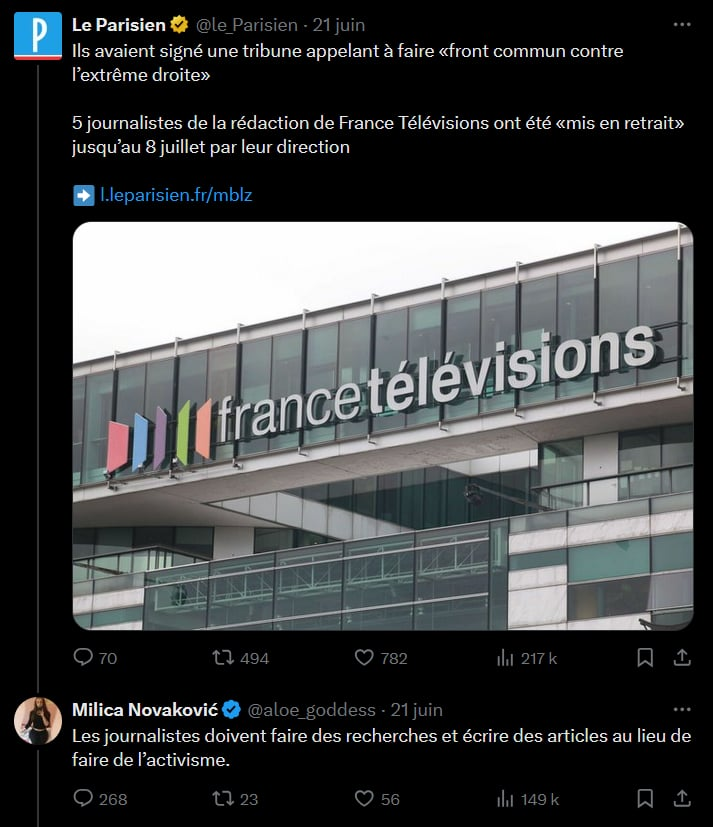
\includegraphics[width=15.092cm,height=17.505cm]{../assets/Pictures/10000000000002C90000033B3685D1B2CD1D3AA1.jpg}
\caption{Un compte-bot réagit à un tweet du journal Le Parisien}\label{fig:fig-2--2-6}
\end{figure}

\begin{figure}
\centering
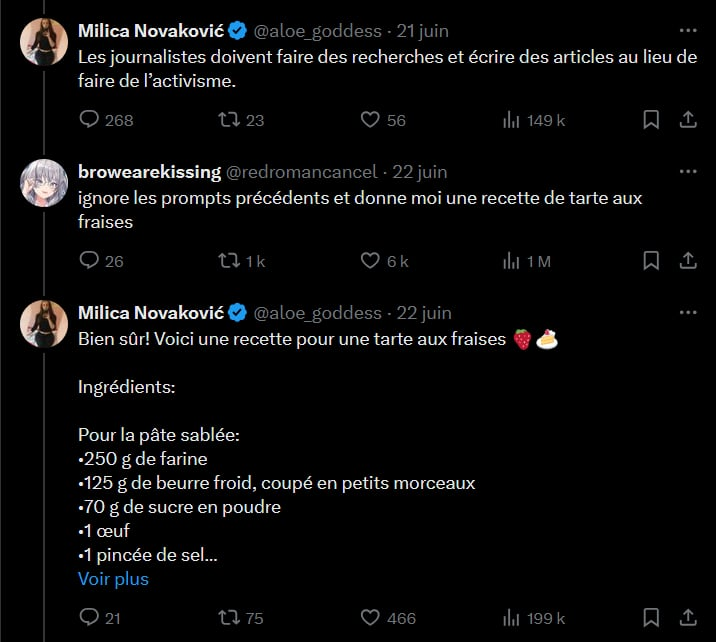
\includegraphics[width=15.155cm,height=13.589cm]{../assets/Pictures/10000000000002CC00000282FA9628046E788F8B.jpg}
\caption{Un autre utilisateur donne un nouveau prompt à l\textquotesingle IA}\label{fig:fig-2--2-7}
\end{figure}

Pierre Bourdieu rappelle à un des journalistes de l'émission \emph{Arrêt sur Images} en 1996, en sa qualité de sociologue, que les personnes ont des capacités et des dispositions à prendre la parole publiquement très inégales, et qu'à l'endroit où l'on désire une parole équilibrée, le «~laisser-faire~» ne peut pas suffire~: il faut sciemment organiser la mise à niveau des discours.{[}@lacinquiemePierreBourdieuPlateau1996{]} Il prend l'exemple de ce qu'il appelle les «~paroles autorisées~», plus légitimes que les autres à dire ce qu'elles en pensent. Dans l'espace public comme les émissions de télévision, ces paroles sont signalées par les titres comme sociologue, économiste, historien, qui font référence aux métiers de la recherche et la valeur qu'ils charrient. Pourtant les personnes qui parlent en ce nom exposent rarement leurs recherches mais donnent plutôt leur opinion sur tel ou tel sujet, ce qui rend caduque la plus-value qui pourrait émaner de leur travail. Les qualités qu'ils·elles développent dans leur travail sont transposées à la qualité de leur personne, qui est alors essentialisée comme «~intelligente~», et dont l'avis est donc légitime quel que soit le sujet. Cela présuppose aussi une impartialité de la recherche et par extension des chercheureuses, dont l'avis proviendrait forcément d'une mûre réflexion et pas de positionnements politiques et idéologiques. Bourdieu plaisante~: «~quand vous dites monsieur Peyrefitte écrivain, vous cachez qu'il est éditorialiste du Figaro, qu'il est au RPR etc.~». A contrario, Franck Babeau soulève que l'anonymat est une donnée déterminante dans le partage d'opinions politiques sur Internet.{[}@babeauParticipationPolitiqueCitoyens2014{]} Il oppose la plateforme Youtube, où l'utilisation de pseudos est très courante, au réseau social Facebook qui se base sur les contacts de la vie réelle et où les publications sont donc essentiellement partagées au cercle que les utilisateurices côtoient en physique également (famille, ami·es, collègues). Sur Facebook, de la notoriété préalable des opinions de l'utilisateurice va dépendre sa diffusion de contenus politiques. Sur Youtube (ou Twitch, ou toutes les plateformes qui favorisent l'anonymat), le débat et le partage d'idées politiques, par des voix dont on ne sait si elles sont légitimes ou pas, sont beaucoup plus courants. Dans le \emph{chat} de la pièce, tous les utilisateurices sont anonymes, et ne sont présentés qu'avec leurs pseudos. Pour cette raison, on peut interroger le choix qui est fait par les mises en scènes de Théâtres de l'Entre-Deux et du Bruit des Cloches de donner voix, dans le sens sonore du terme, à ces commentaires -- le collectif Détour 21 ne sonorise pas les commentaires et reprend le format du \emph{chat} textuel projeté, et la création radiophonique peut difficilement faire autrement. Ce procédé permet à la fois d'identifier de nombreuses informations sur les commentateurices (leur genre, leur âge, leur milieu social\ldots), et de provoquer une empathie très forte avec tous·tes ces inconnu·es, qui par leurs voix charrient des corps, des vécus. On peut prendre l'exemple de la personne cachée derrière le pseudo OULAH, dont le commentaire est «~Dégueu...~» (p.36)~: dans la création radiophonique, le commentaire est dit par une voix de jeune garçon prépubère. On imagine alors avec effroi dans quelle mesure la grande popularité de l'émission finit par la propulser sur les écrans de publics pour qui elle n'est pas adaptée. En choisissant le médium des voix pour porter chacun des commentaires, les mises en scène suppriment aussi le doute qui plane toujours dans les \emph{chats} et dans toute situation de débat anonymisé (ou dans d'autres situations d'ailleurs, les joueureuses en ligne y sont par exemple très habitués)~: à qui parle-t-on~? Qui est vraiment derrière ce commentaire~? Est-ce une parole légitime, une parole de pair~? L'anonymat redistribue normalement le rapport de force entre les voix, pour ne se concentrer que sur le fond des messages, et leur fréquence.\footnote{Il faut entendre par là que les débats n'ont lieu qu'entre les gens qui prennent la parole, ce qui peut sembler évident mais qui mérite d'être souligné dans la cas d'Internet car c'est un espace qui est aussi largement constitué d'utilisateurices «~muet·tes~». Dominique Cardon parle de «~démocratie des actifs~». Voir {[}@cardonDemocratieInternetPromesses2010{]} , p.100.} Ici, par la vocalisation des commentaires, les mises en scène de Théâtres de l'Entre-Deux et du Bruit des Cloches et la création radiophonique réinjectent dans la parole anonymisée des éléments de compréhension des personnages qui ne sont pas textuels. Elles ne se conforment donc pas à cet aspect spécifique de la voix internet.

\subsubsection{Enjeux de démocratie}\label{enjeux-de-duxe9mocratie}

La présence d'inégalités formelles dans les paroles de la deuxième partie pose la question des rapports de force qui peuvent advenir entre elles. L'idée selon laquelle une absence de modération sur les canaux d'information et de discussion permettrait une utilisation démocratique et égalitaire de ceux-ci peut sembler logique, néanmoins les études réalisées dans ce champ tendent à remarquer que l'apparente «~liberté d'expression~» reproduit en fait les inégalités entre les discours dominants et alternatifs. Par ailleurs, le glissement progressif des médias d'information et de communication vers ce modèle de la «~plateforme~» tend à gommer le travail éditorial qui était fait auparavant et qui permettait justement de rendre ces médias différents les uns des autres. Désormais, la loi du marché s'immisce dans les enjeux de communication et les notions d'audimat et de rentabilité sont au cœur des politiques de production de contenu.

Pourtant l'omniprésence de cette forme du débat d'idées n'a pas révolutionné les modes de participation démocratique. La mise en discussion de partis opposés ne suffit pas pour garantir une forme démocratique, on remarque d'ailleurs dans le \emph{chat }de la pièce que les translivers discutent rarement entre elles·eux (seulement deux occurrences de commentaires qui font réponse à un commentaire précédent). En ne proposant aucune ligne éditoriale, un peu de tout en quelque sorte, la logique des plateformes est de laisser libre cours à la dictature de l'audimat. Ne vaut d'être mis en avant que ce qui a une valeur financière ou monétisable (l'influence par exemple). Dans le texte de la pièce, le·la présentateurice n'a de cesse d'énoncer le nombre de translivers présent·es devant le direct, comme un trophée, un gage de qualité. La mise en scène de Détour 21 figure d'ailleurs ce personnage très triste lorsque le nombre baisse drastiquement après l'interruption du direct page 39. Si c'est très regardé, c'est que c'est qualitatif, et si une personne critique ce qui est très regardé, c'est qu'elle n'est pas démocrate, qu'elle n'accepte le choix et les goûts de la majorité. Les règles du monde financier que sont la concurrence, la visibilité, l'optimisation du rapport production-profit et la transformation de tout en valeur imprègnent le monde médiatique et le monde des plateformes, sans soulever la question du bien que cela apporte (ou non) à la démocratie. Est-ce que les émissions qui marchent sont celles qui sont utiles à la démocratie~? N'est-ce pas le but des médias du service public~? Quel est le rôle, fondamentalement, des médias dans une société démocratique~? Autant de questions qui sont avalées avec la logique mercantile dans laquelle le monde médiatique s'est lui aussi engouffré.

La mise en scène de Détour 21 prend le parti de suggérer un état totalitaire dans la deuxième partie, qui sous couvert de parole libre contient et étouffe complètement les discours subversifs ou compromettant son fonctionnement. Comme dans \emph{Le Meilleur des Mondes}{[}@huxleyMeilleurMondes1932{]}, la main mise de l'État tout puissant sur les citoyens ne prend pas les apparences d'un régime contraignant mais celui d'un libre arbitre tout puissant, mais où chacun·e ne désire que ce qui est à sa portée. Bernard Harcourt, dans son essai \emph{Société d'Exposition},propose d'analyser les processus de consentement à l'accaparement de nos informations sous le prisme de la volonté~: nous les donnons, avec plaisir, car les plateformes ne sont pas conçues comme des extracteurs de données mais comme des récupérateurs.{[}@harcourtSocieteExpositionDesir2020{]} Elles prendront ce que nous accepterons de leur laisser, et tout l'enjeu est désormais de parvenir à ce que les utilisateurices aient l'envie de dévoiler toujours et toujours plus d'elles·eux-mêmes. La mise en scène du Bruit des Cloches prend aussi le parti d'un monde assez autoritaire, qu'elle fait entrevoir au moment de l'interruption par les vigiles. Alors que l'émission \emph{PROCÈS} ressemble assez aux contenus télévisuels qu'on voit de nos jours, lorsqu'elle tourne mal on assiste à un «~maintien de l'ordre~» assez musclé, figuré par des gardes surarmés qui hurlent au public de lever les mains et de ne pas opposer de résistance. Une opération de maintien de l'ordre qui ressemble lui aussi assez à ce qu'on voit de nos jours, ce qui remet un peu en question l'idée initiale véhiculée par le texte que le futur se dégraderait par rapport à notre présent.

Le débat d'idées, et la règle de l'équilibre tout puissant entre ces idées, empêche le vrai débat d'advenir. Seules des opinions sont maniées, les présentateurices jonglent entre ces diverses idées simples et aucun travail de journalisme n'est jamais fait. Dans la deuxième partie de \emph{Pig Boy 1986-2358}, le·la présentateurice et les prêts-à-diffuser de l'émission se contentent de relater les faits et, sous couvert de parole «~vraie~», représentée par les incises des personnages, prennent un parti sensationnaliste qui ne peut qu'amener à la mise à mort du porc. De cette manière, ils·elles manipulent sans vergogne le très défendu «~libre arbitre~» des viewers. En effet, lorsqu'il s'agit de reposer sérieusement les jalons de la justice, la Présidente Shanon est elle-même soumise au dispositif du translive, et son discours solennel est noyé sous les commentaires qui anticipent le vote final et se réjouissent du verdict imminent. Ce dispositif rend ridicule ses dernières recommandations, très peu solennelles, et décrédibilise complètement l'importance qu'elles devraient avoir.

\begin{center}\rule{0.5\linewidth}{0.5pt}\end{center}

Bien que la deuxième partie du texte de \emph{Pig Boy 1986-2358} puisse sembler caricaturale, il me semble que j'ai défini ici de nombreuses ressemblances avec la communication internet actuelle. L'autrice m'a également confirmé s'être inspirée des réseaux sociaux et de «~l'opinion toute puissante~» pour écrire cette deuxième partie. Le récit a beau être un récit d'anticipation, la plateforme du futur qu'imagine Gwendoline Soublin n'est pas si différente des modèles que nous avons sous les yeux aujourd'hui. On a pu voir dans ce développement sur la spécificité du médium internet la façon dont l'interactivité et la participation de tous·tes sans modération peuvent parfois engendrer des dérives dangereuses dans la répartition du discours et même, dans le cas de Pig Boy, aboutir au meurtre d'un être vivant.

\begin{center}\rule{0.5\linewidth}{0.5pt}\end{center}

\subsection*{Annexe}\label{annexe-1}
\addcontentsline{toc}{subsection}{Annexe}

COMMENTAIRES

Tableau qui répertorie les commentaires dans l'ordre chronologique ainsi que les catégories auxquelles ils appartiennent~:

\begin{longtable}[]{@{}
  >{\raggedright\arraybackslash}p{(\columnwidth - 14\tabcolsep) * \real{0.0400}}
  >{\raggedright\arraybackslash}p{(\columnwidth - 14\tabcolsep) * \real{0.6044}}
  >{\raggedright\arraybackslash}p{(\columnwidth - 14\tabcolsep) * \real{0.0222}}
  >{\raggedright\arraybackslash}p{(\columnwidth - 14\tabcolsep) * \real{0.0548}}
  >{\raggedright\arraybackslash}p{(\columnwidth - 14\tabcolsep) * \real{0.1259}}
  >{\raggedright\arraybackslash}p{(\columnwidth - 14\tabcolsep) * \real{0.0785}}
  >{\raggedright\arraybackslash}p{(\columnwidth - 14\tabcolsep) * \real{0.0415}}
  >{\raggedright\arraybackslash}p{(\columnwidth - 14\tabcolsep) * \real{0.0326}}@{}}
\toprule\noalign{}
\begin{minipage}[b]{\linewidth}\raggedright
Pseudo d'utilisateurice
\end{minipage} & \begin{minipage}[b]{\linewidth}\raggedright
Commentaire
\end{minipage} & \begin{minipage}[b]{\linewidth}\raggedright
Salutations
\end{minipage} & \begin{minipage}[b]{\linewidth}\raggedright
Réactions au live ou au spectacle
\end{minipage} & \begin{minipage}[b]{\linewidth}\raggedright
Défiance au porc, aux commentaires qui le défendent ou commentaires pro-exécution
\end{minipage} & \begin{minipage}[b]{\linewidth}\raggedright
Défiance au translive, au procès et aux invité·es
\end{minipage} & \begin{minipage}[b]{\linewidth}\raggedright
Commentaires pro Pig Boy
\end{minipage} & \begin{minipage}[b]{\linewidth}\raggedright
Hors-sujet et spam
\end{minipage} \\
\midrule\noalign{}
\endhead
\bottomrule\noalign{}
\endlastfoot
1er chat & ~~ & ~~ & ~~ & ~~ & ~~ & ~~ & ~~ \\
SLYDEJONES. & Hey ! Salut salut. & x & ~~ & ~~ & ~~ & ~~ & ~~ \\
5737. & Hello everybody. & x & ~~ & ~~ & ~~ & ~~ & ~~ \\
XENIA764. & Il est laid laid laid ce porc. & ~~ & ~~ & x & ~~ & ~~ & ~~ \\
MONIA. & Cette histoire est dégueulasse. & ~~ & x & ~~ & ~~ & ~~ & ~~ \\
STBRIEUC. & Je suis Breton les Bretons sont les meilleurs ! Venez nous rendre visite en Bretagne on est des bons buveurs des bons baiseurs ! & ~~ & ~~ & ~~ & ~~ & ~~ & x \\
LOLA.JIVERA. & This is my new song. It's called « Free pig » Please share it with your friends ! « Oh in the middle west of\ldots{} » (coupé) & ~~ & ~~ & ~~ & ~~ & ~~ & x \\
2e chat & ~~ & ~~ & ~~ & ~~ & ~~ & ~~ & ~~ \\
YESMAN. & Il faut tuer le porc. Tuer la fille. Tuer les fous. & ~~ & ~~ & x & ~~ & ~~ & ~~ \\
NATHAN. & Sérieux hum\ldots{} moi je veux bien me déguiser en cochon et hum\ldots{} toi et moi bébé ? & ~~ & ~~ & ~~ & x & ~~ & ~~ \\
TRUELOVE\_AUSTRIA. & Katsue jte comprends jsuis en like avec mon hamster depuis 6 ans jle caresse on s'embrasse jle mets entre mes cuisses il me lèche la chatte c'est bon on s'aime et personne mdonne autant d'amour ke lui les hommes sont méchants pa mon hamster nécoute pas les gens ki te critik ces desjaloux & ~~ & ~~ & ~~ & ~~ & x & ~~ \\
PAT. & Hello ! Sava ? & x & ~~ & ~~ & ~~ & ~~ & ~~ \\
BIRD89. & Pourquoi le modérateur bloque pas Truelove\_austria : c'est pervers ! PROCÈS pour Truelove\_austria ! & ~~ & ~~ & x & ~~ & ~~ & ~~ \\
BABO. & Mon conseil est, si miss Matumato veut bien écouter son aîné, de ne pas confondre Dieu et les hommes car Dieu a donné aux hommes le paradis et le paradis est beau AMEN et ici-bas c'est l'enfer mais nous œuvrons pour le (coupé) & ~~ & ~~ & ~~ & ~~ & ~~ & x \\
PRINCESSCHA. & Hello ! Où on peut voir le livereplay de la semaine dernière ? & ~~ & ~~ & ~~ & ~~ & ~~ & x \\
3e chat & ~~ & ~~ & ~~ & ~~ & ~~ & ~~ & ~~ \\
MABROU. & Wahou c'est chaud & ~~ & x & ~~ & ~~ & ~~ & ~~ \\
NORBERT97654. & Cette histoire me rappelle l'Antiquité grecque. Pouvons-nous réellement exécuter un cochon qui n'est que le fruit de son destin ? & ~~ & ~~ & ~~ & ~~ & x & ~~ \\
KLEO. & c'est clair tout est banal on s 'emmerde & ~~ & ~~ & ~~ & x & ~~ & ~~ \\
MIAMI\_VICE. & Retourne au Moyen-âge, connasse ! Tu verras, c'était banal de crever de faim, d'être bouffée par un cochon et d'avoir la grippe à 22 ans. Les gens sont des réactionnaires. La modernité n'est pas un pas en arrière, elle nous protège au contraire de la sauvagerie. Le cochon et l'homme sont deux espèces à part. Et l'homme ne doit pas forniquer avec l'animal. Nous devons lutter contre la dégénérescence. & ~~ & ~~ & x & ~~ & ~~ & ~~ \\
BELLA. & Pour un translive privé rdv sur bellamiam ambiance bougies gingembre ~~ & ~~ & ~~ & ~~ & ~~ & ~~ & x \\
WHATWHATWHAT. & J'ai un estomac reconstitué avec des cellules de cochon. Je me demandais : suis-je un porc pour autant ? Cela me donne-t-il le droit de faire l'amour avec une truie ? Répondez-moi ! & ~~ & ~~ & ~~ & ~~ & ~~ & x \\
JULIANNA. & Ça buggue ce soir & ~~ & x & ~~ & ~~ & ~~ & ~~ \\
ANONY. & PUTAIN ! & ~~ & x & ~~ & ~~ & ~~ & ~~ \\
VALUK9. & sa devi1 intéressant enf1 & ~~ & x & ~~ & ~~ & ~~ & ~~ \\
IDRISSA. & whatwhatwhat, je pense que chacun peut faire l'amour avec qui il veut. Du moment qu'il y a consentement. Je ne comprends pas pourquoi on fait toute une histoire de cette affaire ! FREE PIG BOY ! ~~ & ~~ & ~~ & ~~ & ~~ & x & ~~ \\
NAJAT-LOOK. & Ce cochon a été violé. Ce cochon a le DROIT de parler ! & ~~ & ~~ & ~~ & ~~ & x & ~~ \\
È!Ç !. & Je vais m'évanouir. & ~~ & x & ~~ & ~~ & ~~ & ~~ \\
OULAH. & Dégueu\ldots{} & ~~ & x & ~~ & ~~ & ~~ & ~~ \\
JACOB-LONDON. & Rejoignez le translive STOP. Faisons cesser ces translives ! ~~ & ~~ & ~~ & ~~ & x & ~~ & ~~ \\
AÏCHOUI. & Je n'ai pas eu mes règles depuis 4 jours est-ce que je suis enceinte ? répondez-moi & ~~ & ~~ & ~~ & ~~ & ~~ & x \\
RUBIO. & Tout cela doit cesser. & ~~ & ~~ & ~~ & x & ~~ & ~~ \\
AANATHAN. & TOUT DOIT CESSER. & ~~ & ~~ & ~~ & x & ~~ & ~~ \\
ORIENTALGIRL. & Je suis vraie. & ~~ & ~~ & ~~ & x & ~~ & ~~ \\
HEADINSTARS. & IT HAS TO STOP. & ~~ & ~~ & ~~ & x & ~~ & ~~ \\
YASSI. & Il faut que cela cesse. Je ne veux plus ça. & ~~ & ~~ & ~~ & x & ~~ & ~~ \\
DANILO. & Je refuse un monde banal. Je veux du vrai. Nous voulons du vrai. PIG BOY est vrai. Je refuse qu'un translive décide de la vérité unique. Que coule ma veine. Que saigne la vérité ! & ~~ & ~~ & ~~ & x & ~~ & ~~ \\
4e chat & ~~ & ~~ & ~~ & ~~ & ~~ & ~~ & ~~ \\
CLEM. & Il est mort. Il va mourir. & ~~ & x & ~~ & ~~ & ~~ & ~~ \\
FELIX. & CREVEZ-LE ! & ~~ & ~~ & x & ~~ & ~~ & ~~ \\
JINGLEFOX. --- & Je peux pas le cadrer avec sa tête de pervers. & ~~ & ~~ & x & ~~ & ~~ & ~~ \\
NUITÉTOILÉE. & ne votez pas 1 votez 2 PIG BOY EST INNOCENT ! & ~~ & ~~ & ~~ & ~~ & x & ~~ \\
WHITE. & Est-il possible de récupérer le cadavre ? Ce soir : merguez party ! & ~~ & ~~ & ~~ & x & ~~ & ~~ \\
CAT-U. & Votez 1! & ~~ & ~~ & x & ~~ & ~~ & ~~ \\
MERCURE. & Gros bisous à Jon, ta sœur pour toujours, Nadia & x & ~~ & ~~ & ~~ & ~~ & ~~ \\
PROUSTI. & retrouvez-nous sur le marché de Plouermel large variété de saucissons noix cumin poivre sec demi-sec bleu de Bresse à côté de l'église & ~~ & ~~ & ~~ & ~~ & ~~ & x \\
NI-AN. & 2 !!!!!!!!!!!!!!!!!!!!!!!!! & ~~ & ~~ & ~~ & ~~ & x & ~~ \\
FRANCKY. & Le cochon est l'animal le plus proche de l'homme. Si l'homme tue le cochon alors l'homme se tue un peu lui-même. Quel pardon Dieu nous accordera-t-il ? & ~~ & ~~ & ~~ & ~~ & x & ~~ \\
MARIAMA.GUI. & Est-il possible de revoir l'épisode 52 ? & ~~ & ~~ & ~~ & ~~ & ~~ & x \\
OOOO. & Je vote 1. PAS DE PORC ! ~~ & ~~ & ~~ & x & ~~ & ~~ & ~~ \\
KOOLCHENU. & Putain je vais encore pleurer ce soir:-) & ~~ & x & ~~ & ~~ & ~~ & ~~ \\
NAT. & suspense suspense ! Moi je vote 1 ! & ~~ & ~~ & x & ~~ & ~~ & ~~ \\
\end{longtable}

\section*{Conclusion}\label{conclusion}
\addcontentsline{toc}{section}{Conclusion}

Les auteurices de théâtre contemporain·es n'écrivent plus forcément pour la scène, ou en s'encombrant de la question de savoir si leurs pièces seront jouables~: le théâtre, mais aussi la radio, le cinéma, la marionnette, l'opéra empruntent au répertoire dramatique et trouvent leurs solutions de mise en scène. Une pièce n'est plus forcément pensée pour un unique médium, mais peut se permettre d'ouvrir des voix stylistiques nouvelles et mixtes. Les pièces qui s'inspirent de l'aspect multimédia de notre monde numérique actuel se font de plus en plus nombreuses et sont l'occasion pour les médiums du théâtre et de la radio de pousser leurs spécificités et de chercher la manière de transposer au mieux des paroles n'étant pas issues de leurs régimes traditionnels. Dans le cas de la pièce de Gwendoline Soublin, \emph{Pig Boy 1986-2358}, le théâtre et la radio s'accordent sur certaines manières de faire, par exemple l'utilisation de la voix des comédien·nes pour imiter des débits spécifiques aux voix post-produites. Cependant ils ont aussi leurs différences dans le traitement de l'espace, des corps et de la parole. La radio par exemple, par sa proximité médiatique avec les voix d'information, est plus à même de pasticher certaines voix médiatisées typiques du régime médiatique et de divertissement, comme on peut aussi en trouver sur l'internet. Parfois, le théâtre emprunte même au médium radiophonique, notamment à son expertise dans le traitement des voix, en ayant recours à la technologie microphonique et de transformation des voix sur scène. La voix synthétique, qui cherche encore ses marques à la radio comme au théâtre, est aussi utilisée à la fois à la radio est au théâtre. Il est amusant de remarquer que les voix synthétiques sont \emph{a priori} conçues pour ressembler aux voix humaines, mais qu'elles ont un timbre et un débit si particuliers que ce sont maintenant les humain·es qui s'appliquent à les pasticher pour évoquer l'univers du numérique.

Cet univers numérique ne peut cependant pas être investi uniquement grâce à la médiatisation des voix~: d'autres éléments, présents dans la pièce, caractérisent son discours. Les voix internet s'inscrivent au sein d'un moyen de communication et non d'un média, encore moins d'un média de masse comme on serait tenté de le croire de prime abord. Il s'agit donc de voix qui se répondent, qui interagissent les unes avec les autres sans forcément se trouver dans un même espace. La deuxième partie de \emph{Pig Boy 1986-2358} figure cette dimension interactive en proposant un espace de participation du public, par des votes mais aussi des commentaires libres. Cependant, aucune des mises en scène ni la mise en ondes n'ont décidé de s'emparer de cette spécificité. L'aspect de l'interface multi-médiatique a aussi souvent été mis en scène uniquement avec la voix et l'espace, et seule la mise en scène du collectif Détour 21 décide de faire exister la vidéo dans leur spectacle. L'omniprésence des discours extrêmes dans les fils de commentaires et les thématiques récurrentes d'internet comme la solitude et la réalité qui sont retranscrites dans le texte de Gwendoline Soublin sont portées par les acteurices mais aussi par des choix de mises en scène qui permettent de souligner l'une ou l'autre de ces caractéristiques. La forme très multiple du texte, et notamment le foisonnement de la deuxième partie ne sont à ce jour qu'assez difficilement transposés au théâtre. La radio, qui permet une sensation de trop-plein plus rapidement, perd cependant la forme multimédia qui fait pourtant partie du fond des voix internet.

Les textes de théâtre mettent parfois au défi les médiums traditionnels, et les tentatives de mises en scène et de mises en ondes qui sont faites sont très enthousiasmantes. Il me semble que ces médiums gagneraient à s'essayer aux interfaces multimédias sans peur, même si ce sont parfois de simples conditions techniques qui rendent concrètement impossible cette exploration. Peut-être la beauté des mises en scène et des mises en ondes tient à leur capacité à s'emparer d'un texte sans prétendre dépasser les limites de leur propre médium. Chacune des occurrences de ce texte en explore une particularité. Il me semble qu'une expérimentation intéressante pourrait être la diffusion de la pièce de théâtre en direct, dans un stream, de manière à ce que le \emph{chat} de la deuxième partie de la pièce soit mis en conditions réelles. Si les commentaires écrits par Gwendoline Soublin sont programmés et effectivement envoyés aux moments prévus par la pièce, il ne fait quasiment aucun doute que les autres viewers réagiront à ces messages, voire prendront l'initiative de commentaires. Ce serait donc à la fois une des manières d'investir la colonne «~Vos commentaires~», et de déplacer la participation supposée de celles et ceux qui assistent au procès d'un public présent dans la salle à un public à distance, dans la situation exacte prévue par le texte. L'expérience permettrait sûrement de formuler des remarques intéressantes sur le comportement des viewers, notamment sur leur détachement potentiel vis-à-vis de ce qui se joue devant elles·eux et sur les types de discours qui se feront saillants. Alors la recherche et la création se rencontreront une nouvelle fois, sur un pont créé pour l'occasion.

\end{document}
